\documentclass[11pt,a4paper]{article}
\usepackage{a4wide,url,graphicx,wrapfig,multirow,enumitem}
\usepackage[T1,T2A]{fontenc}
\usepackage[russian]{babel}
\usepackage[utf8]{inputenc}

\parindent0cm
\parskip3pt
\setlist{noitemsep}

\title{Осторожно! Таблица технических противоречий}  
\author{Леонид Шуб}
\date{Мюнхен, 2006--2007}
\begin{document}
\maketitle

(90\% пользователей ТРИЗ предпочитают инструмент, которого нет)

\begin{quote}
  Это сборник из 11 эссе, опубликованных в виде серии на сайте
  \texttt{metodolog.ru}, ссылки на отдельные эссе см. на сайте
  \url{https://metodolog.ru/conference.html}.

  Text was compiled by Hans-Gert Gr\"abe, Leipzig, within the WUMM Project
  \url{https://wumm-project.github.io/}
\end{quote}

\begin{flushright}
  «… от недостаточного и потому дурно используемого знания\\ есть лишь одна
  защита -- знание более полное».\\ Станислав Лем
\end{flushright}
\section*{1. Краткий пристрастный обзор истории ТРИЗ и ее развития в западной
  Европе.} 

\subsection*{ТРИЗ на подъеме?}

В последние годы в европейской, в частности, немецкоязычной технической прессе
и в Интернете появляется все больше сообщений о чрезвычайно успешных, порой
просто головокружительных результатах в практике использования \textbf{ТРИЗ} и
отдельных ее инструментов. Методика откровенно расхваливается на все лады как
исключительно последовательная и эффективная. Одновременно все больше
производственных предприятий и консультационных фирм пытаются с двух сторон --
как инструмент и как товар -- использовать содержащийся в ней потенциал и
накопленный опыт.

В то же время, интенсивное распространение и развитие ТРИЗ в центральной
Европе происходит со значительным отставанием от аналогичных процессов в США и
Израиле (в среднем на 7--10 лет) и отличается несколькими характерными
особенностями. Прежде всего, это языковые барьеры. Еще в 90-х годах многие
специалисты из Советского Союза, живущие и работающие сегодня в Европе, языком
будущей страны проживания не владели \cite{Shub2004}. Процесс переселения
специалистов из Союза происходил в значительной степени спонтанно. Кто-то
попал в европейский университет как аспирант в рамках программы обмена кадрам.
Другого пригласили еще в ГДР преподавать на год-другой, да так и забыли
вернуть обратно после объединения двух Германий. Кому-то посчастливилось
попасть в контингент политических беженцев или просто удачно жениться. В
списке ТРИЗ-Мастеров, составленном Альтшуллером, 12 имен приписаны к США,
четыре -- к Израилю, и лишь одно -- к Англии. Ни один из активно действующих
ТРИЗ-специалистов не переселился первоначально в какую-либо из промышленно
развитых стран Западной Европы по приглашению на работу, связанную с ТРИЗ.

Методические материалы, учебная и популярная литература по ТРИЗ поступали в
Западную Европу поначалу в основном из США. Претерпевая двойной перевод, и по
ходу неизбежно преобразовываясь, истолковываясь и дополняясь издателями на
свой вкус, издания эти нередко имели лишь отдаленное сходство с русскоязычными
оригиналами и не могли претендовать на адекватность изложения, восприятия и
понимания.

Европейские ТРИЗ-специалисты из числа «аборигенов» жестко ориентированы на
минимальный срок обучения и «производственной» практики, но максимальную
прибыльность практической деятельности. Прочитав первую книгу или прослушав
первый вводный семинар, они сами определяют свою готовность к использованию
методики и, зачастую поспешно, пытаются опробовать свои силы в пилотных
проектах и обзорных семинарах. Эта тенденция порождает порой абсурдные и
комичные ситуации: Иной инженер, окрыленный мощью приобретенного в результате
экспресс-обучения инструментария, смело и уверенно называет себя специалистом
по ТРИЗ. А, прочитав вторую книгу и проведя пару-тройку вводных семинаров, он
уже берется за написание собственной книги по теории. В целом это приводит не
только к многочисленным разночтениям и новым «пониманиям» методики, но
зачастую и к значительной девальвации ее как продукта, к снижению
акцептабельности ТРИЗ-ного движения в целом.

Например, Rolf Herb прослушал в США в 1996 году первый вводный семинар, после
чего перевел с английского и издал в 1998 году года книгу американского
ТРИЗ-трио Тернинко-Зусман-Злотин «ТРИЗ. Путь к успешному продукту, не имеющему
конкуренции» \cite{Terninko1998}.  Эта книга имела на тогда еще пустынном
немецкоязычном рынке немалый успех. Уже через два года R. Herb в соавторстве с
Thilo Herb и Veit Kohnhauser издал уже собственную книгу «ТРИЗ,
систематический путь к изобретению» \cite{Herb2000}, выдвинувшую его на фоне
организованных им же обзорных семинаров в число наиболее часто упоминающихся
ТРИЗ-специалистов Европы.

Скорость перехода от новичка к опытному методисту вызвала бы у всякого
читателя, знакомого с темпами аналогичных процессов в Советском Союзе,
искреннее уважение. Но… В том же 2000-м выходит в свет еще одна книжка
«Находить идеи, развивать продукты с ТРИЗ» \cite{Gimpel2000}, качество
материала в которой можно охарактеризовать не иначе, как
посредственное. Бросается в глаза, прежде всего, откровенная пресыщенность
этого издания иллюстрациями на основе \textbf{TechOptimizer 2.5} (программного
продукта «Invention Machine«) и ссылками на эту программу. Таким образом,
одному новичку удалось в течение года «запустить» на околотризную орбиту еще
трех новоиспеченных специалистов, теперь уже авторов книг по методике
изобретательства.

Призрак сертификации по Европе тогда еще не бродил. Всякий эрудированный
технарь, способный без ошибки произнести слово «ТРИЗ» и привести несколько
примеров использования приемов, принимался за специалиста по решению проблем.
Впрочем, до появления «детей изобретателя Альтшуллера» дело не дошло --
большинству «новых тризовцев» для полной убедительности не доставало владения
русским языком. Все же оценка добросовестности работы того или иного
специалиста до сих пор остается вопросом сугубо субъективным. Уже сама
выработка критериев такой оценки в значительной степени усложняется условиями
консультационной деятельности и статусом консультантов в Европе.

В большинстве стран центральной Европы, прежде всего в Германии, Австрии и
Швейцарии наибольшее распространение имеют два основных вида договоров
подряда. Это так называемые Dienstvertrag и Werkvertrag. Под Dienstvertrag
понимается договор на оказание различных услуг. Работа в рамках такого
договора оплачивается обычно строго в соответствии с отработанным у заказчика
временем. Werkvertrag предполагает выполнение четко оговоренной задачи -- чаще
всего технического характера -- с оплатой при достижении поставленной цели.
Деятельность консультационных организаций всевозможных профилей (а только в
Германии таких фирм с числом сотрудников от двух-трех до нескольких сотен
насчитывается более 10 тысяч) оговаривается, как правило, рамками
Dienstvertrag.  Оплата в этом случае производится на основании размера
дневного гонорара и зависит от числа участвующих консультантов и заранее
оговоренной длительности проекта. Консультант-исполнитель, как правило, не
берет на себя ответственность за успех проекта, а его фирма не несет никаких
издержек в случае неуспеха его деятельности (за исключением редких случаев
полного провала, когда проект прерывается досрочно). Одной из допустимых форм
наказания недобросовестного консультанта является устная анти-пропаганда услуг
его фирмы. Однако, реальной угроза такого наказания остается по-прежнему
только в небольших странах, таких, как Австрия или Швейцария -- с традиционно
крепкими соседскими и родственными связями между фирмами. В Германии, Италии
или Франции риск прослыть нерадивым или неумелым консультантом значительно
ниже. В особенности сомнительной представляется такая возможность в Германии,
где дискретность и охрана данных возведены в ранг национальной политики, и
зачастую даже опытные специалисты вынуждены действовать чуть ли не анонимно.

К сожалению, далеко не всегда тот или иной консультант, называющий себя
специалистом в ТРИЗ, отвечает этому званию. Сомнительным представляется порой
и соответствие предлагаемых иными экспертами ТРИЗ-инструментов реальным
требованиям, предъявляемым к современным механизмам совершенствования
технологических и производственных процессов, решения технических проблем или
развития новых продуктов. Подавляющее большинство начинающих консультантов
редко задаются вопросом о том, какие же из приемов и операторов действительно
являются «работающими», а что можно отнести скорее к средствам РТВ (развития
творческого воображения) или приемам «преодоления психологической инерции». В
основном это касается тех, кто получил тризное образование в последние
пять-десять лет, когда поверхностные знания альтшуллеровской методики стали
все больше входить в моду, зачастую превращаясь в ширму для ушлых продавцов
компьютерных программ, базирующихся на отдельных элементах ТРИЗ. Клейма
«сделано Альтшуллером» зачастую уже достаточно для слепой веры в эффективность
и работоспособность любого отдельно взятого элемента методики. Подавляющее
большинство западных тризовцев искренне уверены, что весь инструментарий ТРИЗ
принадлежит уму и перу одного человека. Как написал бы сегодня поэт «Я говорю
ТРИЗ -- подразумеваю Альтшуллер! ТРИЗ и Альтшуллер -- близнецы-братья!»

Здесь позволим себе отвлечься от основной темы и окунуться в глубины истории.

\subsection*{Сколько родителей у ТРИЗ?}

Автором методики традиционно считается Генрих Саулович Альтшуллер -- советский
(по гражданской принадлежности), узбекский (по месту рождения), русский (в
соответствии с языком, на котором думал, говорил и писал), азербайджанский (по
стране проживания), еврейский (по национальности родителей и особенностям
мышления), карельский (по республике, которая его приняла в последние годы
жизни) писатель-фантаст, инженер и патентовед. ТРИЗ, как не раз подчеркивал и
сам Г.С. Альтшуллер, была его творением. В связи с этим нередко приходилось
слышать от него нарекания в адрес специалистов, открыто предпринимавших
попытки улучшить, расширить и модернизировать методику или объединить ее с
другими методами творчества. Эти поначалу разрозненные попытки начали
принимать форму самостоятельного явления уже в период снижения творческой
активности самого патриарха, совпавшего по времени с перестройкой и
«демократизацией всего» в СССР.

После ухода Учителя процесс «переосмысления» приобрел лавинообразный характер,
все более усугубляющийся многоязычностью тризного сообщества. Ведь еще 20 лет
назад одной из основных преград на пути повсеместного распространения ТРИЗ
являлась проблема адекватного перевода оригинальных материалов и издания их на
языке той или иной страны. Сегодня же все менее вероятной представляется
систематизация новых разработок в ТРИЗ, появляющихся на десяти основных языках
и лишь частично переводящихся на английский. Не говоря уже о том, что многие
«зубры» тризного движения не в состоянии провести экспертную оценку новых
материалов ни на одном другом языке, кроме русского.

Вполне понятно, что протестующие голоса чаще всего раздаются из рядов верных и
искренних последователей Альтшуллера, небезосновательно считающих классическую
ТРИЗ самодостаточной, как по объему наработанного материала, так и по степени
разработки инструментов. Во всяком случае, достаточной для успешного решения
самых разнообразных проблем технического характера. И уж точно, не требующей
радикальных дополнений или переработки. Будучи углубленными специалистами, в
практической деятельности они зачастую территориально ограничены пределами
России и лишь незначительно влияют на деятельность «островных колоний«, то
есть русскоязычных тризных сообществ других стран. Явление это, несомненно,
временное и ослабнет уже через 20--30 лет. Если думать только о детях, то
такая перспектива не может не радовать.

Как бы там ни было, потребность и основания для переосмысления положений ТРИЗ
в свете ее исторического развития возникали регулярно и неоднократно. Сегодня,
лучше зная подоплеку непростой истории рождения и становления методики и
располагая более обширными материалами из общественных и частных архивов,
можно сказать (и даже утверждать), что ТРИЗ была \textbf{и его}, Альтшуллера,
творением.  (Как Октябрьскую Революцию вряд ли уместно называть творением
Ленина, не упоминая Плеханова, Троцкого, Зиновьева, Сталина и многих других
теоретиков и практиков революционного движения). И величайшие достижения, и
обидные недостатки этой теории несут на себе отпечатки личностей ее
основателей и созидателей. Вот что писал об этом сам Альтшуллер: 
\begin{quote}
  Методика изобретательства обобщала опыт изобретателей, и естественно, что
  еще в период ее разработки мне пришлось беседовать, консультироваться,
  дискутировать с очень многими новаторами. Это были разные люди: по
  изобретательскому стажу, техническому кругозору, специальности, способностям
  и склонностям. Их объединяло одно: стремление создавать новое. И не
  удивительно, что, ознакомившись с методикой, еще только создаваемой, они
  стремились тут же ее использовать, а потом вносили поправки, предлагали свои
  дополнения. Особенно значительный вклад в развитие методики внесли инженеры
  Р. Шапиро и Д. Кабанов. \cite{Altshuller1961}
\end{quote}

Уже поэтому истоки ТРИЗ следует искать, прежде всего, в личностях ее
основателей, их соратников и учеников. История возникновения ТРИЗ -- это, не в
последнюю очередь, хронологически расставленные этапы развития их собственных
представлений о путях и возможностях развития механизмов мышления. Эти люди --
признанный автор Генрих Альтшуллер и малоизвестный соавтор Рафаил Шапиро (Фото
из Фонда Г.С Альтшуллера\footnote{\url{http://www.altshuller.ru/photo/}}),
совсем неизвестный соратник Д. Кабанов, жена и верная помощница Г. Альтшуллера
Валентина Журавлева и многие другие мыслители. Это их увлечения и
разочарования, гениальные идеи и не менее гениальные заблуждения. То, что
большинство этих людей по разным причинам «вышли» из процесса создания
методики еще до начала ее повсеместного признания, не дает оснований считать,
что из самой ТРИЗ ушли и их «мозги«, исчезли или потеряли значение найденные
ими идеи и предложенные концепции, сделанные ими разработки, совершенные
ошибки или недостигнутые цели.

Действительно, общепризнанным автором АРИЗ -- основного комплексного
инструмента ТРИЗ -- считается Генрих Альтшуллер. Признанным, но не
единственным. 

\begin{quote}
  Создание и тем более совершенствование АРИЗ нельзя приписывать одному
  человеку. Идею создания рациональной системы решения изобретательских задач
  в 1946--49 гг. поддерживал Дмитрий Дмитриевич Кабанов, главный инженер
  инспекции по изобретательству Каспийской военной флотилии. Оценивая
  изобретения, Д.Д. Кабанов применял принцип: максимум результата при минимуме
  затрат. Этому принципу могли удовлетворить только те изобретения, которые
  являлись преодолением технических противоречий. Таким образом, одно из
  важнейших исходных положений алгоритмической теории решения изобретательских
  задач формировалось под влиянием взглядов Д.Д. Кабанова на изобретательскую
  деятельность. \cite{Altshuller1974}
\end{quote}

\begin{wrapfigure}[16]{l}{5cm}\vspace*{-1em}
  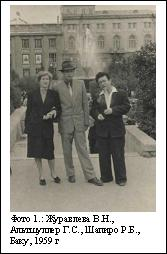
\includegraphics[width=.3\textwidth]{./1.jpg}
\end{wrapfigure}
Биографов Альтшуллера трудно упрекать в недостаточно тщательном изучении
планов занятий первого курса АзОИИТ (Азербайджанский общественный институт
изобретательского творчества) 1973--74 гг. Как и в том, что они не обратили
внимания на имя человека, фактически подарившего методике понятие технического
противоречия.  Вряд ли справедливо будет упрекнуть и самого Кабанова в
недостаточном участии при создании и разработке новой методики. Но его участие
еще можно представить как выполнение должностных обязанностей.

Особого внимания заслуживает личность Рафаила Шапиро и его вклад в разработку
ТРИЗ и ТРТЛ. Не только потому, что он был другом, ровесником и одноклассником
Генриха Альтшуллера. И не потому, что вместе они создали и запатентовали свои
первые изобретения и написали первые статьи. И даже не потому, что Шапиро
многие годы являлся наиболее близким коллегой-писателем, одним из активнейших
популяризаторов молодой методики. Но, прежде всего, потому, он был одним из ее
основоположников, генератором идей и катализатором творческого процесса. Если
уж многие сравнивают создание ТРИЗ с революцией в изобретательстве, то Шапиро
следует отнести к числу ее пламенных революционеров, незаслуженно вычеркнутых
из исторических разделов учебников.

\begin{quote}
  В 1948--49 гг. непосредственное участие в разработке первых вариантов АРИЗ
  принимал Рафаэль Борисович Шапиро (Р. Бахтамов). Он участвовал также в работе
  на протяжении 1956--59 гг. \cite{Altshuller1974} 
\end{quote}
Другими словами, Шапиро был полноправным соавтором эффективных, лаконичных и
четких вариантов алгоритма -- АРИЗ-56 и АРИЗ-59. Впрочем, в те годы он еще
упоминался в качестве соавтора \cite{Altshuller1956, Altshuller1959}.

Из воспоминаний самого Генриха Альтшуллера можно сделать вывод, что прочность
тандема Альтшуллер-Шапиро основывалась, прежде всего, на значительной
полярности характеров, увлечений, мировоззрений и жизненных целей, которая
притягивала и объединяла двух молодых изобретателей на пути к достижению общих
целей. Годы войны, неудачи первых лет совместного изобретательства, аресты и
допросы, лагерные скитания -- ничто не смогло разделить их, разбить их
духовное единение. Серьезные сложности начались тогда, когда наметились первые
успехи, когда методика начала получать признание. Один из очевидцев этой
неустанной борьбы противоположностей вспоминает: 
\begin{quote}
  Рафик был умнее Альтшуллера. Генрих был ярче, но Рафик был умнее. Он вообще
  был очень умный человек, даже мудрый. Когда он работал в журнале «Страна и
  мир» (мюнхенском издании русских эмигрантов, в котором Шапиро, живший в
  Иерусалиме, многие годы являлся ведущим экономическим и политическим
  обозревателем -- прим. автора), то шутили, что Горбачев принимает решения,
  только прочитав статьи Рафика. Если в журнале издавались две его статьи, то
  одна шла под именем Бахтамова, а другая -- Шапиро.
\end{quote}

Альтшуллер мыслил более конкретными категориями. Работоспособному и
энергичному, ему нравилось действовать, выдавать продукцию, получать
результаты: 
\begin{quote}
  Первое авторское свидетельство на изобретение я получил (совместно с
  Р.Б. Шапиро и И.В. Тальянским -- Л.Ш.)... в школе, когда заканчивал десятый
  класс. После школы я стал студентом Азербайджанского индустриального
  института.  Казалось бы, полученные в институте знания помогут вскоре
  сделать и другие изобретения. Однако прошло много лет, прежде чем мне выдали
  второе авторское свидетельство. За эти годы я отправил 103 заявки на
  изобретения. И получил 103 отказа». \cite{Altshuller1961}
\end{quote}
Альтшуллер был готов перечитывать десятки тысяч описаний изобретений, чтобы
упорно расширять Список Основных приемов (сначала до 50, а затем и дальше) и
стандартов, число параметров в Таблице и т.д.

Шапиро же больше привлекала деятельность, скорее подходящая под определение
грандиозной, гениальной, потрясающей все устои. Именно он явился инициатором
того злополучного письма «товарищу Сталину». Письмо это, к сожалению, до сих
пор не опубликованное, в свое время было разослано более чем в 40 адресов и,
согласно общеизвестной версии, явилось одной из причин многолетнего заключения
обоих друзей в тюрьмах и лагерях. 
\begin{quote}
  У Шапиро возникла мысль написать письмо Сталину. Надо сказать, для него это
  характерная реакция вообще. Когда он проникался сознанием величия чего-то,
  ему хотелось быстро внедрить и получить результат…. Шапиро был потрясающий
  оптимист». \cite{Altshuller1986}
\end{quote}

Информация о создателе ТРИЗ Генрихе Альтшуллере зачастую пересыщена элементами
научно-фантастического и даже героического оттенка, и это не удивительно, ведь
речь идет о биографии профессионального писателя-фантаста.  «В 14 лет он имел
несколько патентов на собственные изобретения. В 20 лет стал профессиональным
патентоведом, экспертом Каспийской флотилии в Баку. Потом он создал новую
науку.»\footnote{Г.С. Альтшуллер, Центральный Еврейский Ресурс.
  \url{http://www.sem40.ru/famous2/e428.shtml}.  2020 no more online -- HGG}.
Так называемым популяризаторам не столь важно, что первая успешная заявка была
сделана с двумя соавторами в 17 лет, а подтверждение пришло двумя годами
позднее. Что больше сотни последовавших за нею заявок были отклонены. Что
«профессиональный патентовед и эксперт», в 20 лет только что бросивший учебу в
институте, «имел все основания считаться крупным авторитетом в области плохих
изобретений» \cite{Altshuller1961}. Что о создании новой науки утверждать,
мягко говоря, преждевременно. Важно, чтобы было красиво.

В подавляющем большинстве исторических справок о ТРИЗ говорится, что письмо
Сталину написал Альтшуллер. Иногда добавляется «вместе с другом». Очень редко
упоминается имя друга. Все же, читая воспоминания Альтшуллера, трудно
отделаться от ощущения, что ему так и не удалось разделить ответственность за
этот поступок поровну: «Я несколько раз отговаривал его (Шапиро, -- Л.Ш.),
когда дело касалось изобретения, а вот здесь...» На этом месте люди, близко
знавшие Альтшуллера и испытавшие на себе сложности его характера, лишь
недоверчиво пожмут плечами. Как, впрочем, и при упоминании других случаев
добровольно-принудительного следования желаниям Рафика Шапиро. Прецедентов
согласия Альтшуллера с чьим-либо мнением, принципиально расходившимся с его
собственным, пока еще никто не припоминал. Тем более, невозможно представить
себе Генриха Альтшуллера в роли исполнителя чужой воли.

Об испытаниях, выпавших на его долю в Бутырской тюрьме и лагерях, о допросах,
на которых его уговаривали признать собственную вину и оклеветать Альтшуллера,
Рафаил Шапиро написал в своих воспоминаниях, уже живя в Израиле. Но так и не
собрался их опубликовать. Лишь спустя два года после его смерти эти записи
были изданы его супругой Норой в небольшой книге «Двадцать пять плюс двадцать
пять». В сумме 50 -- столько должно было исполниться Рафику в день
освобождения в соответствии с приговором суда, который -- по иронии судьбы или
чьему-то «тонкому» расчету -- был оглашен в день его рождения 13-го января
1951 года. Книга, название которой его близкий друг Владимир Портнов,
написавший предисловие, дал уже без него, так и не была закончена. Понимая,
что умирает, Шапиро уничтожил многие черновики и архивные материалы.

Отношение Р. Шапиро к Г. Альтшуллеру и их совместной работе можно было бы
определить, скорее, как трепетное обожание и самоотречение. Вот только один
характерный штрих: В 1961 году Р. Бахтамов (литературный псевдоним Рафаила
Шапиро) издал сборник рассказов «Изгнание шестикрылого серафима», в котором
воспевал заслуги Альтшуллера по созданию новой методики. В том же году Генрих
Альтшуллер в своей книге «Как научиться изобретать» уместил роль Шапиро на
протяжении почти 15-летнего совместного пути в одну строчку, оценив его как
«особенно значительный вклад» в развитие его, Альтшуллера, методики. Впрочем,
и этот вклад Альтшуллер разделил на двоих: Шапиро и Кабанова. По
справедливости.

Было ли случайностью, что работу по непосредственному составлению Таблицы
приемов преодоления технических противоречий, (которую по праву можно отнести
к наиболее трудоемкой, хотя и наименее творческой части усилий по созданию
комплексной методики), Альтшуллер начал лишь после того, как Шапиро
практически «вышел из игры«? А до этого… «Шапиро очень быстро оценил нашу
перспективу… вытекающую сторону. Он сказал так: 
\begin{quote}
  Маркс вывел законы развития общества, Дарвин вывел законы развития живых
  организмов, \textbf{а мы выведем теорию, которая даст миру законы развития
    технических систем}. … То есть он первый оценил эту штуку, это очень
  важно. Масштаб ее понял \cite{Altshuller1986}.
\end{quote}
Эти слова Альтшуллера появились не в его книгах или статьях, и не в 1961 или
1965. Вклад Шапиро был оценен по заслугам лишь в 1986 году при записи мемуаров
Альтшуллера в частной беседе с одним из его учеников.

С уходом Шапиро из общего дела по времени совпадает и увлечение
Г.С. Альтшуллера идеей создания «Эвротрона» (первой механической
«изобретающей» машины, как ее представляет Фонд Г.С Альтшуллера). Об этой
истории нам известно пока очень мало. Зато достаточно очевидной представляется
каталитическая роль «Эвротрона» в появлении на свет Таблицы
противоречий. Механический изобретатель требовал и легко жующегося
«механического» питания.

В общем, если отвлечься от революционной тематики и признать Альтшуллера
полноправной «матерью» ТРИЗ, выходившей и воспитавшей ее, (то есть по-прежнему
считать, что «родил» методику именно он), то Шапиро, скорее, был ее духовным
отцом, покинувшим семью в пубертатный период их общего ребенка и вскоре
лишенным прав отцовства.

Лишь через два года после смерти Шапиро -- в канун своего 70-летия --
Альтшуллер впервые называет некоторые даты, касающиеся бывшего соратника и
друга: 
\begin{quote}
  \textbf{Шапиро Рафаэль Борисович} (литературный псевдоним -- Бахтамов Р.Б.)
  присоединился ко мне в 1942 году (когда Генриху было 16 лет, -- Л.Ш.),
  вместе кончили десятый класс, вместе пошли на нефтемеханический факультет
  Азербайджанского индустриального института. Первое зарегистрированное
  изобретение -- тоже общее. И срок отсидки в ГУЛАГе тоже нам отмерили поровну
  -- по 25 лет. Выпустили нас тоже в один день -- 23 октября 1954 года.
  Освободившись, Шапиро проработал в ТРИЗ по 1961-й год. Ушел из жизни в 1994
  году.  \cite{Altshuller1996}
\end{quote}
Совместная работа над разработкой ТРИЗ ушла в прошлое, но бывшие соратники еще
не расстались. Теперь уже под псевдонимами писателей-фантастов они продолжали
спорить о путях развития методики творчества. Именно в рассказах и повестях
Г. Альтова и Р. Бахтамова можно наиболее последовательно проследить
становление личностей и мировоззрения этих наиболее значительных
основоположников ТРИЗ.

\begin{quote}
  Перегнать науку тяжело, -- говорит писатель Р. Бахтамов. … Пусть не обидятся
  на меня товарищи по перу, но, на мой взгляд, предметом
  научно-фантасти\-ческой книги должна быть не техническая проблема, а, прежде
  всего \textbf{человеческие идеи, человеческие проблемы, короче, человек
    будущего мира}.  Тогда это будет настоящая литература.

  Альтов, возражая Бахтамову, добавляет:

  Но для того, чтобы сказать о будущем человеке, нужно сказать, \textbf{где он
    живет, в каком мире}. И от того, как мы развиваемся, как мы идем к этому
  будущему миру, от того, каков технический прогресс -- от этого зависит,
  каким показать человека. …

  Р. Бахтамов написал новую книгу «Властелин оксимира». Фантаста увлекла
  человеческая идея: что будет с таким качеством, как героизм, если его не
  нужно будет проявлять? \cite{Amnuel964}
\end{quote}
Возможно, что принципиальные разногласия писателей Р. Бахтамова и Г. Альтова
во взглядах на развитие научно-фантастической литературы сыграли свою роль в
том, что имя Шапиро на многие годы практически перестало упоминаться в
материалах по ТРИЗ.

Как бы там ни было, но Рафик Шапиро сошел с дистанции, подобно многим другим.
А Альтшуллер остался и продолжил работу. На протяжении полувека именно он
являлся организатором и координатором, связующим звеном, аккумулятором
информации и движущей силой общего процесса, который сегодня уже традиционно
воспринимается последователями как «создание ТРИЗ». Уже поэтому тот сгусток
идей, опыта, но и неизбежно наработанных стереотипов, который мы называем
«классической ТРИЗ», это в значительной степени и его увлечения, гениальные
идеи и отчаянные заблуждения. Это и победы Альтшуллера над собственной
инерцией мышления, свойственной гениям в не меньшей степени, чем их
предшественникам и современникам, только, быть может, распознаваемые на
значительно более высоком уровне. Это и его ошибки, в которых ему так нелегко
было признаться даже самому себе, от которых было так трудно, порою просто
невозможно, отказаться. Ошибки тем более обидные, что они потребовали многих
лет жизни -- сначала для их созидания, а после -- для исправления или
«забывания». Отдавая дань гению Альтшуллера, мы все же не обязаны слепо
следовать и его гениальным ошибкам, маскируя их под достижения в трепетном
стремлении сохранить лицо и укрепить авторитет Учителя. Не признавать ошибки
-- значит, создавать новые, все более дорогостоящие и трудно исправимые.

Важно подчеркнуть, что ТРИЗ -- это наиболее успешная, но не завершенная
попытка привести в систему все многообразие мыслительных механизмов многих
поколений изобретателей, которые кропотливо и настойчиво собирал, развивал,
проверял и использовал на протяжении своей жизни Генрих Саулович Альтшуллер.
Поэтому методика образца 80-х во всем ее многообразии отражает, прежде всего,
динамику развития личности, процессов мышления и изменения взглядов на эти
процессы самого Альтшуллера. Известны лишь немногие отдельные случаи признания
им каких-либо значительных изменений или дополнений, предлагавшихся более
юными последователями. В частности, Альтшуллер долгое время настаивал на своей
неограниченной монополии на «производство» и развитие АРИЗ.

ТРИЗ не является законченной «методикой поиска новых идей» для всех и каждого,
но скорее трафаретом, образцом, набором кубиков-элементов, с помощью которых
каждый может скроить себе свою систему развития талантливого мышления на
основе исходных установок, собственного жизненного опыта, сложившихся
стереотипов и поставленных задач. Теоретически «законченной» она могла бы
стать для ее авторов. Но с уходом Альтшуллера развеялась последняя надежда и
на это. Незавершенными останутся Общая теория сильного мышления (ОТСМ) и
Теория развития творческой личности (ТРТЛ). Создание Теории Сильного Мышления
преобразовалось в некую надсистемную Достойную Цель, столь же идеальную, сколь
недостижимую в рамках жизни отдельно взятой личности или одного поколения. И
неспроста серьезное изучение ТРИЗ неизбежно перекликается с осмыслением
истории ее создания.

ТРИЗ как методика, основанная на синтезе приемов и алгоритмов, отражает модели
мышления, свойственные различным творческим личностям в самые разные периоды
их жизни и деятельности. Именно это обстоятельство объясняет тот факт, что
даже опытные и заслуженные специалисты не используют, не воспринимают, а порой
и отвергают отдельные элементы ее инструментария. Нередки случаи стихийного
«переосмысливания», наивного упрощения отдельных элементов, вынужденного
возврата к уровню 30-40-летней давности. С другой стороны, некоторые операторы
и приемы, даже сам АРИЗ, порой дополняются и развиваются энтузиастами из числа
«новых тризовцев». Эти представители коммерциализированного поколения зачастую
даже не имеют понятия о том, что этот путь однажды (а то и не раз) уже был
пройден другими.

Но вернемся к нашим табличным вопросам.

\subsection*{Таблица умножения современного изобретательства?}

Авторами многих публикаций об использовании методики и рекламных объявлений
являются,согласно аннотациям, опытные ТРИЗ-специалисты с многолетним стажем
практической работы. Какие же инструменты-кубики выбирают для себя современные
последователи и «разработчики» ТРИЗ на Западе? Отчего порой в качестве
универсальных средств предлагаются сомнительные, морально безнадежно
устаревшие инструменты? Так в большинстве материалов речь идет о
\textbf{Таблице приемов устранения технических противоречий} (далее --
\textbf{Таблица}) и традиционно относящихся к ней 40 приемах их преодоления.
На Западе она известна больше как «\textbf{Матрица противоречий}»
(Widerspruchsmatrix, Contradiction Matrix), на Востоке как «\textbf{Таблица
  умножения}». С середины 90-х по сей день, она остается излюбленным и
наиболее известным, чаще других упоминающимся и успешно используемым
«инструментом» ТРИЗ. Интернет пестрит сообщениями и рекламными объявлениями,
подобными приведенным ниже (Вставка А).

С легкой руки российских экспортеров ТРИЗ и американских, а затем европейских
любителей изобретательства Таблица в буквальном смысле пошла по рукам.
Сногсшибательный эффект от ее использования обнаруживают специалисты в самых
разных областях деятельности. Наиболее свежими членами «Клуба любителей
Таблицы» стали бизнесмены \cite{Leon2005}, архитекторы \cite{Mann2005a},
музыканты \cite{Mann2005b} и банкиры \cite{Stuart2005}. В очереди на прием в
Клуб стоят массажисты, диск-жокеи и стоматологи.

Сегодняшняя ситуация в Европе отдаленно напоминает положение вещей в СССР
60-70-х годов, когда молодая методика с большим трудом пробивала себе дорогу в
ученых и бюрократических кругах. Таблице, благодаря математической стройности,
внешней простоте и убедительности, удалось в те годы примирить многих ярых
противников методики с фактом существования ТРИЗ.

Но метаморфозу, происходящую с ТРИЗ в Европе начала 21-го века трудно назвать
развитием. Скорее, это неуклонное упрощение и стремительная деградация
классической методики с постепенным распадом на отдельные наглядные и легко
продаваемые «кирпичики». В наши дни у нее появляется все больше сомнительных
друзей и почитателей, стремящихся переиначить и перекроить ее. Попытки
компенсировать кажущуюся им сложность ТРИЗ или непонимание отдельных ее
инструментов достигаются путем самых различных «обрезаний», созданием новых
«упаковок» и псевдоалгоритмов. Лишь за последние годы появились варианты
«упрощенной» ТРИЗ: Meta-TRIZ, TriSolver-ARIZ, SIT (Систематическое
Инновационное Мышление), ASIT (Передовое СИМ), USIT (Универсальное СИМ) и
другие. Появление подобных мутантов, казалось бы, должно мобилизовать
последователей Альтшуллера на организованную защиту методики и своих рядов.
Вместо этого все большее число тризовцев попадают под знамена новоявленных
«модернизаторов». Вырвавшись из-под «железного занавеса» бывшей тризной
империи, методика растеряла большую часть своей изначально романтической
мотивации и превратилась в расхожий товар. Европа вступает в эпоху Т-ТРИЗ --
Табличной ТРИЗ.

Декларируемое назначение Таблицы -- облегчить, как для начинающего
пользователя, так и для опытного решателя выбор приемов разрешения типовых
противоречий для решения конкретной задачи. Ставшая в Европе символом ТРИЗ,
громоздкая и труднообозримая Таблица, в действительности, не только в
значительной степени усложняет и удлиняет поиск решений, но зачастую
окончательно заводит пользователя в тупик, исключая возможные решения целиком
из поискового поля.

Уже в период своего создания Таблица фактически не являлась работающим
инструментом. А ведь именно благодаря массированному применению Таблицы и
изобретательских приемов, ТРИЗ в последние годы все чаще приравнивают к
«структурированному мозговому штурму». Внешне четкий и наглядный инструмент,
Таблица вкупе со Списком Основных приемов содержит в себе множество острых
противоречий, основополагающих заблуждений, сводящих даже теоретические
возможности ее использования для целенаправленного решения технологических
проблем к нулю.

Предпринимаемые в последнее время все чаще попытки представить ТРИЗ как некую
панацею при любых недугах технического или социального характера, в
значительной мере вредят как самой методике, ее развитию и распространению,
так и ее носителям -- ТРИЗовцам. За этими попытками в большинстве случаев
стоит все та же Таблица противоречий! И если для 90\% технарей, знающих о
методике понаслышке, Таблица является ее символом, то для большинства знатоков
она олицетворяет или ее вчерашний день, или ее сегодняшнюю деградацию и
стремительный развал тризного движения, некогда представлявшего собой
изысканное сообщество интеллектуалов.

Предлагаемая серия статей предостерегает, прежде всего, промышленных
заказчиков и начинающих пользователей методики от поспешности при выборе
инструментария. Это и призыв к осмотрительности, как при заключении договоров
на оказание консультационных услуг, так и в вопросах приобретения программных
продуктов на базе ТРИЗ, предлагаемых сегодня на европейском рынке. Статьи
содержат многие малоизвестные факты из истории создания методики и отдельных
ее элементов, в том числе «постоянного и полномочного представителя» --
Таблицы технических противоречий. Сопоставление фактов и цифр наглядно
демонстрирует несостоятельность Таблицы как рабочего инструмента в целом, так
и как вспомогательного механизма для интенсификации поиска решений для
несложных проблемных ситуаций в частности. Становится очевидной и
необоснованность выбора ее в качестве информационного фонда при создании
ТРИЗ-базируемых программ для «изобретающих машин», что ставит под вопрос
практическую значимость и эффективность использования большей части
компьютерных «изобретающих» программ и их составляющих, предполагающих в любой
форме применение Приемов на основании «табличных» рекомендаций.

В «\textbf{Проекте требований для оценки уровня подготовленности заявителей
  при аттестации в МА ТРИЗ}» \cite[Приложение 2]{MATRIZ2003} большое внимание
уделено следующим вопросам:
\begin{itemize}
\item 2 уровень; Знать основные блоки истории ТРИЗ, как науки -- таблицу и 40
  приемов преодоления технических противоречий, основные этапы развития АРИЗа.
  Иметь представление о дополнениях или изменениях, внесенных другими
  специалистами по ТРИЗ. Уметь оценивать уровень и инструментальность этих
  изменений.
\item 3 уровень; Знать ход развития ТРИЗ, основные изменения в теории, начиная
  с первых публикаций, понимать причины и закономерности этих изменений.
\end{itemize}
Предлагаемые материалы рассчитаны, таким образом, и на всех желающих
приобрести сертификат 2-го, 3-го уровня и выше -- вплоть до «Мастера ТРИЗ».

\subsection*{Вставка А: Таблица приемов преодоления технических противоречий в
  Интернете} 

«ТРИЗ предлагает быстрый и целенаправленный поиск решений, помогает
классифицировать техническое противоречие с помощью параметров и основных
приемов целевым порядком». Martin Fritz (Universitat Stuttgart) предлагает
дополненную Таблицу противоречий в своей работе «Потенциальный анализ
относительно объединения методов ТРИЗ и бионики» по цене EUR
24,99\footnote{\url{http://www.hausarbeiten.de/faecher/vorschau/39753.html}}.

«Снижение себестоимости при помощи Таблицы противоречий» обещает Thomas
Schlos\-ser\footnote{\url{http://www.triz-online-magazin.de/ausgabe03_03/artikel_4.pdf}}.

Таблица противоречий предлагается при использовании Изобретательского Решения
проблем в Requirements
Engineering\footnote{\url{http://www.fb9dv.uni-duisburg.de/se/de/education/ws0405/RE/SaschaBrink(2004)SemRE-TRIZ.pdf}}.

«В основе всех технических решений лежат 40 так называемых изобретательских
приемов. Через выявление противоречий в системе может быть проведен
целенаправленный поиск решений». «Таблица противоречий, как известнейший из
инструментов ТРИЗ, и относящиеся к ней абстрактные шаги» рассматриваются в
серии семинаров
\textbf{SUPPORT}\footnote{\url{http://www.stenum.at/download/folder_support.pdf}}.

«Одним из самый известных инструментов ТРИЗ-методики является Таблица
противоречий», хвалит Dr. habil. oec. Dipl.-Ing. Petra Rietsch. Применение
Таблицы при создании нетехнических новшеств можно изучить на семинаре «Анализ
деловых моделей е-бизнеса малых и средних
предприятий»\footnote{\url{http://www.wu-wien.ac.at/kmb/lehre/sbwlneu/vk52}}.

Преимущества и недостатки \textbf{Таблицы} сравнивает \textbf{INVENTNET® GmbH}
на своей
странице\footnote{\url{http://www.inventool.de/toolauswahl/tooldescription.php?id=123}}.

«В особенности, начинающим ТРИЗовцам рекомендуются 40 изобретательских приемов
для преодоления технических противоречий и система их применения в форме
Таблицы противоречий как инструмента для легких и средней тяжести
изобретательских задач («Свободная Обучающая Платформа для изобретателей и
разработчиков«). Работа с приемами здесь начинается с 10 лучших принципов для
мозгового штурма\footnote{\url{http://www.triz.it/ebf/tct03.htm}}.

Johannes Maierhofer (Future Management) представил на 4. Конгрессе ТРИЗ
анализ, в котором в качестве «лучших» методов, соответствующих требованиям
новаторского проекта, были признаны QFD, системный анализ процессов и Таблица
противоречий, поддерживаемые программой Logic Mind
Guide\footnote{\url{http://www.triz-online.de/triz_magazin/ausgabe05_03/artikel_5.htm}}.

\clearpage
\begin{flushright}
  «Сейчас 40 приемов имеют лишь историческое значение«\\
  Г.С. Альтшуллер \cite{Altshuller1985}
\end{flushright}
\section*{2. Самый главный инструмент!}

По окончании моего доклада на 4-м Конгрессе ТРИЗ (Frankfurt/Main, 30.06.2005)
мне было задано несколько вопросов. Два из них звучали (в переводе на русский
язык) так: «Работая в проекте, Вы анализируете задачу, формулируете
техническое противоречие, выбираете по Таблице приемы, а дальше?» После моего
замечания о том, что Таблица не является инструментом для решения
производственных задач, и я не пользуюсь ею, а Альтшуллер уже 30 лет назад
придавал ей лишь историческое значение, в зале возникло тягостное молчание.
Чувствовалось, что сидевшие в зале участники были шокированы ответом. Вопросов
мне больше не задавалось. Не о чем было спрашивать! Ну, в самом деле, о чем
можно говорить с человеком, не использующим в работе Таблицу?!

Вот так у меня появился повод разобраться с феноменом «Таблицы приемов
преодоления технических противоречий». А заодно и окончательно выяснить для
себя смысл ее существования. Уж не пропустил ли я за 20 лет, прошедших с
последнего учебного семинара, какие-то революционные разработки в этом
вопросе? Уже просматривая странички в Интернете, восхваляющие «подзащитную», я
понял, что гораздо эффективнее будет сделать харакири под плакатом
«\textbf{НЕТ -- Таблице!}» на очередной Конференции ETRIA в Граце, чем
пытаться обратить «мирным путем» внимание европейской тризной общественности
на существование (вернее, фактическое отсутствие) проблемы. (Собственно, этим
теперь и приходится заниматься).

\begin{center}
  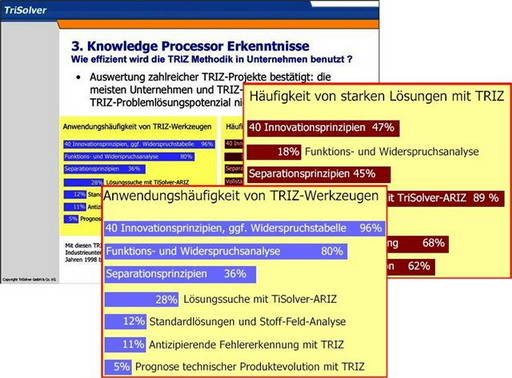
\includegraphics[width=.8\textwidth]{./2.jpg} \\
Рис. 1. Частота применения инструментов ТРИЗ фирмой TriSolver\\ и их успешность
в 1998--2005 годах (на опыте работы с 38 предприятиями)
\end{center}

В докладе консультационной фирмы TriSolver «Новаторство как процесс» на этом
же Конгрессе \cite{Livotov2005} (материал снят с сайта!)  предлагается
сравнительный анализ частоты использования и эффективности наиболее
значительных инструментов ТРИЗ по результатам многочисленных проектов,
проведенных этим консалтингом в 1998--2005 годах на 38 промышленных
предприятиях Европы (Рис. 1). В большинстве своем это известные и уважаемые
имена, многие из которых (DaimlerChrysler, Philips Semiconductors, Infineon
Technologies, Siemens Dematic и др.) названы на сайте
фирмы\footnote{\url{http://www.trisolver.de/software/innovationssoftware.htm}}.

«Таблице противоречий и 40 изобретательским приемам» (40
Innovationsprinzipien, ggf. Widerspruchstabelle) отводится в этом реестре
абсолютное первое место по уровню симпатий клиентов. С 96\%-ой частотой
используются они в проектах, проводимых TriSolver! Убедительно лидируя среди
коллег-инструментов, Таблица значительно опережает функциональный анализ
(Funktions- und Widerspruchsanalyse, 80\%) и выглядит совсем недостижимой для
таких «мало востребованных» инструментов, как принципы разделения физических
противоречий (Separationsprinzipien, 36\%) или вепольный анализ, включая
стандарты (Standardl\"osungen und Stoff-Feld-Analyse, 12\%). Даже поиск
решений с участием «фирменного» \textbf{TriSolver-ARIZ} (значительнее звучала
бы разве что только «TriSolver теория относительности«) занимает с 28\% лишь
четвертое место по важности. Старушке Таблице удалось переплюнуть по частоте
использования всю замыкающую список пятерку инструментов, включая
прогнозирование и «диверсионный анализ» (AFE).

В половине случаев (47\%) применения Таблицы и приемов специалистам фирмы
удается -- следуя диаграмме -- получить «сильные» решения. Хотя выход таких
решений пока еще на 40\% ниже, чем при решении проблем по TriSolver-ARIZ,
общее количество их для Таблицы при ее практически повсеместном использовании
все же в два раза перекрывает результаты, достигаемые алгоритмом, и в три раза
-- принципами разделения физических противоречий. Успехи вепольного анализа на
фоне «табличных» заслуг выглядят просто смехотворными.

Фирма TriSolver является, по утверждению ее представителей, ведущей на
немецкоязычном рынке по оказанию консультационных услуг и разработке
компьютерных программ в области ТРИЗ и системного новаторства. Было бы логично
предположить, что эта фирма прилагает все усилия для популяризации методики
(как в целом, так и отдельных ее инструментов) в различных отраслях
промышленности, расширяя и развивая свой собственный арсенал. В
действительности же, почти все приведенные в диаграмме «классические»
инструменты потеряли только за один год от 30\% до 50\% пользовательского
спроса (Рис. 2). Все, кроме Таблицы!

\begin{center}
  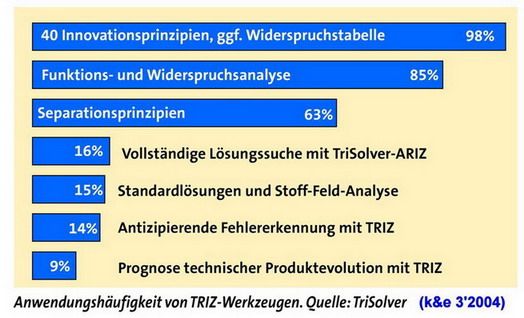
\includegraphics[width=.8\textwidth]{./3.jpg} \\
  Рис. 2. Частота применения инструментов ТРИЗ фирмой TriSolver в 2004 г.
  (Konstruktion \& Engineering, 03/2004).
\end{center}

Особенно примечательным является тот факт, что еще годом раньше принципы
преодоления (разделения) физических противоречий востребовались клиентами
TriSolver в два раза чаще (63\%)! И только применение \textbf{TriSolver-ARIZ}
имело в 2004 году еще более эпизодическое значение, чем нынче -- лишь 16\%. Об
этом говорилось в фирменном отчете о Конференции ETRIA-2004 в
западногерманском городе Aachen \cite{Livotov2004}.

Абсурдной динамика изменения (перераспределения) удельной частотности
использования элементов ТРИЗ в работе TriSolver представляется лишь на первый
взгляд. Она становится значительно понятнее после знакомства с основными
принципами действия единственной на сегодняшний день немецкоязычной программы
\textbf{TriSolver4.net}. В основе ее лежат, конечно же, тризные рекордсмены:
Таблица и 40 основных приемов!

Таким образом, вытеснение интеллигентных и эффективных, но требующих
повышенных затрат времени при обучении (и уже только по этой причине менее
привлекательных) инструментов «универсальной» Таблицей приобретает воистину
промышленные масштабы. Эта тенденция становится все более заметной как у
отдельных консультантов, так и у индустриальных пользователей ТРИЗ, обретая
черты диагноза. А ее лавинообразное ускорение, пусть не всегда такое
драматичное, как у \textbf{TriSolver}, заражает азартом соседей по рынку
консультационных услуг.

Вот выдержка из статьи, с которой имели возможность ознакомиться более 5
миллионов читателей немецкого «Шпигеля» от Канарских островов и «до самых до
окраин» -- Японии и Гонконга:
\begin{quote}
  Томас Байер, шеф исследовательского отдела фирмы Виттенштайн, держит список
  40 приемов постоянно перед глазами. В его бюро они висят на стене рядом с
  Таблицей, которая помогает ему выявить, какое из правил подходит к той или
  иной дилемме \cite{Dworschak2005}.
\end{quote}
Подобного рода «ненавязчивая реклама» все чаще появляется как в технической и
научно-популярной прессе, так и в крупных информационных журналах. Европейцы
еще не забыли, что и другая, не менее важная таблица химических элементов
пришла когда-то с морозного Востока -- а ведь и в ней тоже были незаполненные
клетки! Этот аргумент убеждает.

\begin{center}
  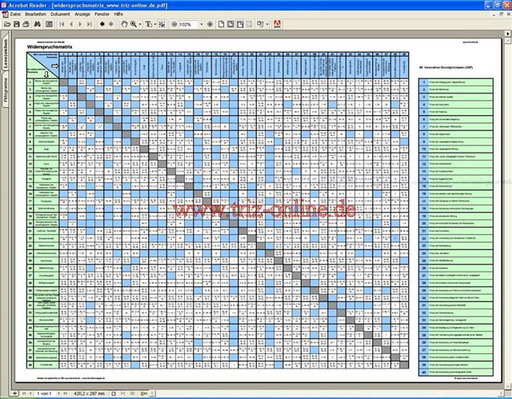
\includegraphics[width=.8\textwidth]{./4.jpg} \\
  Рис. 3. «Классическая» Таблица приемов преодоления технических противоречий
  (АРИЗ-71). Голубым цветом выделены пустые клетки.
\end{center}
Опубликованная на сайте журнала triz-online (Рис. 3) наиболее точная немецкая
версия Альтшуллеровской Таблицы в ее «классической» форме копируется
многочисленными почитателями и знатоками этой части методики в Европе.

Что же это за универсальный инструмент изобретателя, которому с 1998 по 2005
годы отдавали абсолютное предпочтение 38 промышленных предприятий и фирм --
преданные клиенты TriSolver? Мощный инструмент изобретательского мышления --
памятник гению Альтшуллера? Увлекательный калейдоскоп, в котором при каждом
повороте возникают новые занятные сочетания? Забавная игрушка для прожектеров,
помогающая генерировать как явно сумасшедшие, так и сногсшибательно
правдоподобные идеи?

\begin{center}
  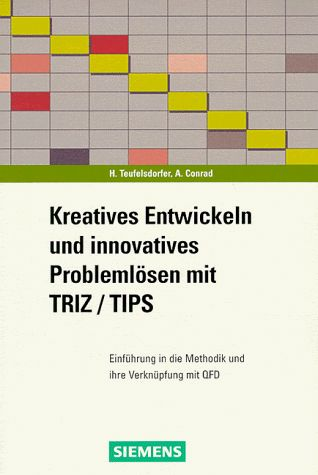
\includegraphics[width=.5\textwidth]{./5.jpg} \\
  Тризная геральдика
\end{center}
В качестве иллюстрации к обложке одного из первых немецких изданий по
TRIZ/TIPS \cite{Teufelsdorfer1998} была выбрана стилизованная Матрица. Именно
она все чаще выдается западными консультантами за «почти всю» ТРИЗ или, по
крайней мере, за ее основной, наиболее четко и безотказно действующий
универсальный механизм. Их утверждения, по крайней мере, статистически не
лишены оснований. У постоянно растущего числа людей разных профессий и
вероисповеданий, национальностей и цвета кожи «русская» методика
изобретательства ассоциируется именно с нею. Если провести опрос всех
европейцев, когда-либо слышавших о ТРИЗ, и поинтересоваться тем, какой образ
рождается в их воображении при ее упоминании, то в 99\% случаев будет получен
контрольный ответ. А вот горящая в голове лампочка Ильича, в России нередко
используемая как символ творческого изобретательского мышления, вызывает у
западного читателя скорее болезненные ассоциации. Роденовский мыслитель,
отдавший за идею последнюю рубашку, тоже не возбуждает: С положениями ЖСТЛ на
вводных и обзорных семинарах не знакомят -- эти материалы упрямо не поддаются
адекватному переводу ни на один европейский язык. Зато Таблица понятна и без
перевода.

Действительно, свобода формулировать многочисленные противоречия с получением
самых причудливых конфликтных пар создает видимость расширенного, хотя и
поверхностного «вылавливания» идей. Именно последнее обстоятельство превращает
применение Таблицы внешне похожим на «офилософствованную» и несколько
систематизированную помесь перебора вариантов с мозговым штурмом. И создает из
нее легко уязвимую мишень для вдумчивых и технически хорошо образованных
критиков. Оно же дает повод убежденным противникам «коммунистических» методов
мышления огульно распространить слабости Таблицы на все остальные инструменты
ТРИЗ. Всякое упоминание о ее диалектических основах и без того вызывает у
простых капиталистов аллергическую реакцию, напоминая о неизбежной
необходимости разрушения всего (их) мира до основанья.

Таблица открыла новую эру в развитии и распространении ТРИЗ на Западе.
Методика в ее лице начала превращаться в продукт изобретательского ширпотреба.
Глубокое и вдумчивое изучение философских основ стало необязательным, как
правило, невозможным, а зачастую и вредным. Все более второстепенное значение
приобретают «громоздкие» варианты последних АРИЗов. Владение Таблицей и
приемами, подкрепленное дюжиной смачных примеров, позволяет увлечь
потенциального клиента ошеломляющей идеей «целенаправленной дистилляции
конфликтующих влиятельных характеристик при изменениях в системе»
\cite{Sietmann2001}. 

Редкий «ТРИЗ-специалист» в Германии рискнет прийти на деловую встречу без
тщательно выглаженной и аккуратно сложенной Таблицы в кармане пиджака. Потому
что если без Таблицы, то каждому ясно, что это -- не специалист. Если
проследить динамику распространения методики в мире, то крамольная мысль об
обратной зависимости среднего уровня владения тризным инструментарием от
общего числа пользователей напрашивается сама собой.

\begin{center}
  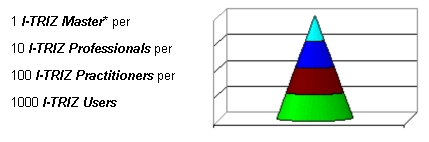
\includegraphics[width=.5\textwidth]{./6.jpg} \\
  Рис. 4. Тризная
  иерархия\footnote{\url{http://www.ideationtriz.com/training.asp}}. 
\end{center}

Воспользовавшись выявленной специалистами Ideation International Inc.
пропорцией между числом простых и непростых пользователей ТРИЗ,
Г.С. Альтшуллер легко определил размеры популяции передовиков
изобретательства. В 1998 году их -- от новичков до Мастеров ТРИЗ -- было чуть
больше 70 тысяч. Обвинять всех Мастеров (на диаграмме -- голубые) в ежедневном
и повсеместном использования Алгоритма было бы неосторожным. Зато вычислить
число абсолютных знатоков Таблицы (зеленые) не составляет труда.

В России 60-х годов она не только олицетворяла собой научный (статистический)
подход в изобретательской деятельности, но еще и играла важную политическую
роль в процессе официального признания ТРИЗ. Идея ее создания была для
Альтшуллера удачной находкой, позволяющей совместить декларируемую точную
алгоритмизацию изобретательского процесса с возможностью использовать богатые
внутренние информационные ресурсы решателя. Она же помогала порой избегать
необходимости расшаркиваться перед инертными теоретиками изобретательства
до-ТРИЗной эпохи. Далеко не все были готовы отказаться от милого сердцу МПиО с
его романтичными, окутанными в золотое вспышками внезапного, но заслуженного
озарения. Кто-то просто боялся высовываться. Ведь не случайно официальная
позиция науки на этот счет десятилетиями практически не развивалась:
\begin{quote}
  Показательны в этом отношении статьи, опубликованные в N2 журнала
  «Изобретатель» за 1929 г. (учитывая, что в период 1937-45 других работ по
  психологии изобретательского творчества не появлялось, можно считать, что
  взгляды, существовавшие в 1929 г., сохранили силу и к 1946 г.)
  \cite{Altshuller1975}.
\end{quote}
О том, что многие сторонники «других взглядов» были элементарно уничтожены,
говорить вслух в 1975 году было еще не принято. Но не знать этого Альтшуллер,
сам прошедший тюрьмы и лагеря, не мог.

Едва появившись на свет, Таблица попала на благодатную почву, словно
специально для нее подготовленную. Советской стране требовались тысячи новых
технических решений. Прежде всего, речь шла об улучшении устаревших механизмов
и дальнейших разработках практически во всех отраслях промышленности.
Поскольку уровень таких инноваций вовсе не обязательно должен был быть
чересчур высоким, -- предпочтительнее были как раз не слишком сложные, но
оригинальные решения, -- приветствовалось быстрое и относительно недорогое
«претворение в жизнь». Поэтому заключенный в строгие табличные формы механизм
«разогрева» инженеров, дающий возможность в непринужденной обстановке одним
стимулировать, а другим симулировать выход на развивающие идеи, пришелся ко
двору.

«Приемы изобретательства были известны и до Г.С.Альтшуллера. Но у него они
были классифицированы (таблица из 40 приемов решения техпротиворечий) и
радикально изменены по структуре» \cite{Murashkovsky2003}. Таблице
удавалось, за счет подкупающей свежести некоторых приемов, соблазнять технарей
необычностью способа интенсификации перебора вариантов. Разложенные по Таблице
в убеждающе неравномерном порядке, приемы играли роль морковок, к которым надо
было тянуться. Волей-неволей приходилось напрягать мозги. В зависимости от
числа сформулированных технических противоречий и уровня общей эрудиции
«тянущихся», таких морковок набиралось от двух-трех до дюжины.

Сегодня лишь небольшая часть коммерческих пользователей ТРИЗ открыто признает
необходимость полного и окончательного отказа от практики одурачивания
клиентов «Гаданием по Таблице». \textbf{Чем же тогда?} -- резонно возражает
значительная масса тризовцев. Но и рьяные сторонники табуляции разделяются на
две конфронтирующие партии: ортодоксов и реформаторов.

По благоговейной тщательности, с которой изобретатели разных стран и народов
оберегают целомудренность Альтшуллеровской Матрицы образца 1971 года,
аккуратно расставляя священные числа от 1 до 40 в нужные клеточки и не
расставляя в ненужные, их можно сравнить, пожалуй, лишь с Хранителями древнего
Пятикнижия. Так приверженцы Кабалы свято верят в божественное происхождение
библейских свитков. Всякое изменение буквенной последовательности, по их
мнению, не только меняет смысл текста, но и приводит к безвозвратной потере
зашифрованных в гигантском буквенном ребусе пророчеств и предначертаний.
Поклонение тризовским скрижалям, включая богослужения перед образами Таблицы с
соблюдением предписанных обрядов, на Западе имеет все шансы перерасти в
устойчивую изобретательскую религию. Читая тут и там об удивительно
целенаправленном и результативном выборе судьбоносных приемов, невольно
вспоминаешь анекдот, в котором старый фельдшер, разламывая пополам таблетку
анальгина, наставлял больного солдата: «Это тебе, сынок, от головы, а это от
живота! Только смотри, не перепутай!» Смешно? Оборот от внедрения анекдота в
производственную практику достиг в последние годы астрономических сумм,
заставляющих подавить усмешку.

«В принципе, можно ткнуть, не глядя, в любой прием, и уже что-нибудь удается
придумать», -- мнение Мастера ТРИЗ Исаака Бухмана поддерживают многие «старые
волки», познавшие бессмысленность Таблицы еще в советские времена.
Бессмысленность, но не бесполезность!

Действительно, тыкать вслепую в список из 40 приемов для обученного (тем
более, сертифицированного) специалиста как-то несолидно. А перебирать их (с
подприемами -- больше сотни) по очереди -- лженаучно! Другое дело -- тыкать в
Таблицу с четырьмя тысячами счастливых номеров, подчиняющимися строгим
статистическим законам, «по науке». Это уже -- профессия!

Особенно плотно смыкаются ряды борцов за «истинную, неделимую и нерушимую»
перед лицом то и дело возникающей опасности со стороны всевозможных
ревизионистов и реформаторов, упорно пытающихся расширить, дополнить,
начистить и раскрасить до боли родную Таблицу 1971 года. Впрочем, до крестовых
походов дело не дойдет. Ситуация, как и положено, подчиняется главному
диалектическому закону -- единству и борьбе. Борьба за истинную веру затмевает
единство принципиального вопроса -- а был ли мальчик? Являлась ли Таблица
вообще когда-то работоспособным и обоснованным инструментом?

Всякий хорошо воспитанный тризовец знает, что к любым утверждениям «классиков»
следует относиться с уважением -- не суть важно, идет ли речь, к примеру, о
пяти тысячах или же двух миллионах изученных патентных документов. Но ведь и
отделять фантастику от реальности в Союзе тоже когда-то учили. Для этого и
инструмент был разработан соответствующий -- Регистр фантастических идей.

Но европейские тризные миссионеры с Регистром не знакомы. Мощь табличного
оружия здесь принимается на веру и традиционно обосновывается
умопомрачительным числом «сильных» решений, легших в его основу. Три четверти
западных популяризаторов ТРИЗ демонстрируют это могущество, словно
сговорившись, на одном и том же примере: Решение задачи об упаковке пиццы,
полученное для американской фирмы Pizza-Hut, приписывается применению
Таблицы. «Альтшуллер идентифицировал на основе изучения 2.5 миллионов патентов
39 технических параметров и 40 изобретательских приемов… А хорошие идеи не
валятся с неба», проповедует Rolf Herb слушателям своего семинара. Добрую
половину интервью для немецкого журнала «Wirtschaftswoche» («Экономическая
Неделя«) он посвящает восторженному разбору этого основательно приевшегося
даже в Европе решения\footnote{Kind im Manne, Wirtschaftswoche Nr.19,
  4.5.2003}.

Другой активный популяризатор Альтшуллеровской методики, ответственный за
обмен технологиями в торгово-промышленной палате земли Хессен и активный
организатор Конгресса во Франкфурте Carsten Gundlach «разжевывает» историю с
Pizza-Hut уже под голландским соусом\footnote{C. Gundlach. Mit Kreativität und
  Strategie zur Nachhaltigkeit. TRIZ Online Magazin 05/2003, no more online --
  HGG.}. Невольно возникает ощущение, что остальные пять примеров,
переведенные из российских и американских книг, не жуются.

Читая в западных источниках об \textbf{огромном}, \textbf{гигантском} или
\textbf{необъятном} патентном фонде, переработанном Альтшуллером при
составлении Таблицы в 1946-65 годах, как и о «доработанных» позднее его
учениками двух или четырех миллионах патентов (с целью подтверждения указанных
в ней приемов), невольно вспоминаешь другой анекдот. О сапожнике, соседями
которого по переулку оказались «лучший в городе» и «лучший в стране»,
повесившем у своей будки табличку «Лучший на этой улице». Чтобы окончательно
закрыть вопрос об объемах учтенной информации, остается лишь заменить термины
местного масштаба «огромный» или «гигантский» на скромный, но со вкусом --
«ВЕСЬ мировой патентный фонд».

\subsection*{Таблица умерла! Да здравствует Таблица!}

К началу 70-х в СССР позиции ТРИЗ стали настолько устойчивыми, что
Г.С. Альтшуллер свою Таблицу в течение почти 30 лет с 1971 и до своей кончины
в 1998 больше не развивал. Поставленную задачу она уже выполнила. Более того,
ее существование постепенно начинало угрожать новой тризовской политике.
Альтшуллер даже предпринял попытку «похоронить» результаты своего многолетнего
труда, объявив в 1975 году, что «появление АРИЗ-71 фактически обесценило
список и таблицу применения основных приемов» \cite{Altshuller1975}.

В любом производстве, начиная от мелкой мануфактуры и заканчивая
автомобильными гигантами, вывод устаревших продуктов из ассортимента связан со
значительными сложностями технического, финансового и социального характера.
Нередко проблемы эти недооцениваются и превращаются в самостоятельное
многолетнее «производство». Случаи, когда с энтузиазмом начатая, но
недостаточно глубоко продуманная модернизация оканчивалась банкротством,
далеко не единичны. Нередки примеры вынужденной замены значительной части
персонала, десятилетиями оттачивавшего свои навыки, не востребованные в новом
производстве. Вопрос о безболезненном выведении Таблицы и приемов из
«производственного процесса» не мог не беспокоить. Ждать пока фирменный товар
не превратится в бельмо на глазу, тоже не хотелось. 
\begin{quote}
  На устарелость таблицы из 40 приемов сам Альтшуллер указывал еще в начале
  70-х. У меня сохранилось письмо Генриха Сауловича от 1976 года, в котором он
  просит меня не включать эту таблицу в мои лекции по ТРИЗ, поскольку «сейчас
  все видится совсем иначе» \cite{Murashkovsky2006}.
\end{quote}
Очень хочется верить, что и это письмо из личного архива Юлия Мурашковского
когда-нибудь будет опубликовано полностью.

Все же эти признания не помешали Генриху Сауловичу посвятить «обесцененным и
иначе видимым» инструментам свыше 30 страниц своей следующей книги «Творчество
как точная наука» \cite{Altshuller1979} -- в два раза больше, чем новому
АРИЗ-77. Правда, во всей своей красе Таблица уже не была напечатана. Зато
призывов обратиться к ней со ссылкой на «Алгоритм изобретения» здесь имелось
более чем достаточно. Противоречие решалось стандартным (для ТРИЗ) путем.
Одним (разработчикам) -- в частной переписке или личных беседах --
недвусмысленно давалось понять, что пользоваться Таблицей больше нельзя.
Другим (простым читателям) -- в книгах и методических пособиях -- она
преподносилась в неизменном виде. Делалось это, конечно же, исключительно в
целях популяризации ТРИЗ. Ну, еще может быть, чтобы сэкономить время на
подготовке новой книги. Назвать это решение элегантным трудно, новым --
пожалуй, что нет. Но методически грамотным -- вполне. Легенда об Аль-Иссе в
табличном варианте. Благо, открывать личико «богиню» никто и не принуждал. В
ее красоту и вечную молодость верили беспрекословно.

Любого рядового тризовца подобные колебания «главной линии» могли бы сбить с
толку. Но простой народ траурная весть, к счастью, не достигла. Копий
«партийных» документов на всех не хватало. Разработчики компьютерных программ,
знакомые с ТРИЗ, расценили слухи о смерти Таблицы как изрядно преувеличенные.
Как бы там ни было, сотни предприимчивых комбинаторов -- и не только
начинающих -- вот уже 30 лет с достойным восхищения постоянством избирают
«бесценную» для исполнения главных ролей в наиболее ответственных трюках. А
десяток-другой посвященных наблюдают за этим цирком, надежно припрятав в
кармане фигуру из трех пальцев. С выходом на европейскую арену Таблица и
приемы предлагаются, наряду со ставшими уже привычными, но все еще дорогими
«изобретающими машинами», в виде плакатов, свитков, видеоклипов, детских
комиксов, слайдов и игральных карт.

«ТРИЗ-Покер с парой кружек пива, проблемой, огромным удовольствием и кучей
гениальных идей» (Фото) -- все обучение занимает ровным счетом три минуты!
«Мозговой штурм станет для Вас незабываемым переживанием», заверяют авторы
игры и рекомендуют закрепить полученные навыки 4-х часовым удовольствием с
профессионалом всего за 590 Euro. Свою миссию они выражают в простой мудрости:
«Людям следует делать то, что они не умеют, но делали бы с удовольствием, если
бы знали, что им это удавалось бы». Под тем, что люди делать не умеют,
подразумевается … страшно подумать!

\begin{center}
  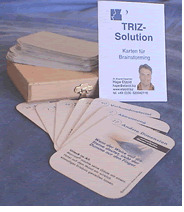
\includegraphics[width=.5\textwidth]{./7.jpg} \\
  ТРИЗ-покер. «Несколько кружек пива, проблема, изобретательность и куча
  гениальных идей. Мозговой штурм будет незабываемым»
\end{center}
Среди покупателей и клиентов -- \textbf{BASF}, \textbf{DaimlerChrysler},
\textbf{Siemens AG}, \textbf{ALTANA Pharma}, \textbf{Apcon/itelligence},
\textbf{Reemtsma}, \textbf{Bertelsmann Stiftung}. Основные партнеры по покеру
на европейском рынке -- Trisolver, MethoSys, TRIZ Journal, Quality Engineers.
Блестящие отзывы для сайта предоставили Отдел Стратегических Продаж
промышленного гиганта «Siemens» и группа развития новых технологий при
Fraunhofer Institut -- крупнейшем научно-исследовательском институте Германии.
Этот же институт подтверждает экономию с помощью карт 3-дневного
ТРИЗ-семинара.  Можно лишь гадать, о семинарах какого уровня ведут речь
уважаемые ученые.

«Новое платье королевы» шьется споро, но с размахом. Обучающие напитки и
радиопостановки -- лишь вопрос ближайшего будущего. А вот чтобы привлечь
покупателей к новому недорогому методическому пособию по ТРИЗ на
конвенциональном (бумажном) носителе, серьезный издатель -- Академия
Технического Университета города Ульм (TQU Akademie GmbH) -- делает в рекламе
особое ударение на прилагаемую «Таблицу противоречий в формате \textbf{А2}»
\cite{Blaesing2001}. Чему посвящены 70 страниц пособия, предназначенного для
руководителей ТРИЗ-проектов и рабочих групп, несложно догадаться.

В одном из писем, датированном 1985 годом, голос Альтшуллера звучит уверенно и
уже почти снисходительно: «Сейчас 40 приемов имеют лишь историческое значение.
Работаем мы -- в основном -- стандартами» \cite{Altshuller1985}.  К этому
письму, адресат которого, к сожалению, неизвестен, еще не раз придется
обращаться. Шутил Генрих Саулович или заблуждался искренне, но только
историческое значение все больше приобретают стандарты. Вечно живыми оказались
приемы и Таблица.

А в Грац я решил не ехать. Непрофессионально выполненное харакири вполне могут
принять за очередной метод активизации творческого мышления. Начнется
организация учебных семинаров…

\clearpage
\begin{flushright}
  Мудрец не кладет все яйца в одну корзину.\\
  (Мигель Сервантес)
\end{flushright}
\section*{3. Древняя история создания ТВППТП}

\subsection*{Так что будем устранять?}

Причины возникновения и логика развития Таблицы, как механизма выбора
подходящих приемов при устранении технических противоречий, до сих пор,
видимо, не представлялись темами, требующими детального рассмотрения.
«Серьезным инструментам» -- ЗРТС, вепольному анализу или Стандартам --
посвящены многочисленные объемные работы. Таблице же -- сухие строчки в
исторических справках. Во всяком случае, очевидно, что подавляющее большинство
разработчиков и поныне придают истории Таблицы значительно меньшее значение,
чем даже истории возникновения и развития типовых приемов. Между тем, было бы
ошибкой считать, что приемы -- в их современном виде -- являлись первичным, а
Таблица -- вторичным или даже второстепенным продуктом, поскольку именно
появление Таблицы не только легитимировало значительное расширение списка
приемов, но и определило их равноправное (а на некоторых этапах и
доминирующее) положение в структуре ТРИЗ.

Здесь следует напомнить о том, что уже сама предыстория появления приемов и
Таблицы представляется достаточно противоречивой. Впервые идея создания
системы последовательных мыслительных операций, в которой поиски способов
устранения технического противоречия (или его причины) велись бы на основе
исследования типичных приемов (прообразов), была высказана основоположниками
ТРИЗ \textbf{Генрихом Сауловичем Альтшуллером} и \textbf{Рафаилом Борисовичем
  Шапиро}. В опубликованной ими в 1956 году программной статье «О психологии
изобретательского творчества» \cite{Altshuller1956} наряду с использованием
уже известных в природе и различных областях техники прообразов, предлагался и
поиск новых приемов (путем изменения известных прообразов на различных
системных уровнях).

Эту статью часто приводят как некий переломный пункт, обозначивший начало
систематической деятельности \textbf{Альтшуллера} (о \textbf{Шапиро} при этом
как-то забывают) над будущей «изобретательской наукой». При этом собственно
статья имела к психологии лишь поверхностное отношение. Зато материал насыщен
большим количеством примеров технического характера, что должно было создать
впечатление компетентности авторов в раскрываемом вопросе, скрывая скорее
дилетантские познания в области психологии.

Статья оставляет двоякое впечатление: С одной стороны, возникает ощущение, что
авторы стремятся воспользоваться моментом и высказать «наболевшее». Читая
строчки с критикой «советского изобретательства, которое связано с плановым
производством», невольно вспоминаешь о том так и не найденном «письме
Сталину», с которого начались злоключения авторов. Несомненно, они стремились
использовать «временные ресурсы». Ведь статья была написана и опубликована уже
через несколько месяцев после того, как 22 февраля 1956 года -- в ходе XX
съезда КПСС Хрущёв выступил с докладом о разоблачении «культа личности»
Сталина.

С другой стороны, учитывая значительные пробелы в советской специальной
литературе в области изобретательского творчества (как отмечали сами авторы,
«единственная монография по этому вопросу в советской психологической
литературе -- книга П.М. Якобсона «Процесс творческой работы изобретателя»
\cite{Jacobson1934} -- была опубликована еще в 1934 г.), нужно было
использовать представленную возможность и «застолбить» те разработки, которые
были проведены за предыдущие годы. Или те, которые хотелось бы
провести. Возможно, по этой причине некоторые темы остались непроработанными,
а сама статья не вызвала широкого читательского резонанса.

Подводя итоги «беглого очерка развития» современного велосипеда, авторы среди
прочего сделали следующие выводы, легшие в основу тезисов первого алгоритма:
\begin{quote}
  \begin{itemize}
  \item[3.] Планомерное развитие системы (машины, механизма, процесса)
    оказывается возможным до тех пор, пока не возникнут и не обострятся
    противоречия между более совершенным элементом и отстающими ее частями.
  \item[4.] Это противоречие является тормозом общего развития всей системы.
    Устранение возникшего противоречия и есть изобретение.
  \item[5.] Коренное изменение одной части системы вызывает необходимость ряда
    функционально обусловленных изменений в других ее частях.
  \end{itemize}
  Следовательно, каждое творческое решение новой технической задачи --
  независимо от того, к какой области техники оно относится, -- включает три
  основных момента:
  \begin{itemize}
  \item[1.] Постановка задачи и определение противоречия, которое мешает
    решению задачи обычными, уже известными технике путями.
  \item[2.] Устранение причины противоречия с целью достижения нового -- более
    высокого -- технического эффекта.
  \item[3.] Приведение других элементов усовершенствуемой системы в
    соответствие с измененным элементом (системе придается новая форма,
    соответствующая новой сущности).
  \end{itemize}
\end{quote}

Практически те же рассуждения были приведены и тремя годами позднее в
следующей совместной статье \cite{Altshuller1959}. Как не трудно заметить,
понятие «изобретение» в смысле «устранение возникшего противоречия» и, как
следствие, «коренное изменение одной части системы» в значительной степени
конфликтует с разработанной соавторами в дальнейшем концепцией ИКР, введенной
уже в АРИЗ-59.  В ней «Идеальный конечный результат -- это ситуация, когда
нужное действие получается без каких-либо затрат (потерь), усложнений и
нежелательных
эффектов»\footnote{\url{http://www.trizland.ru/trizba.php?id=8}}.

Отступая от основной темы, следует все же отметить, что и это -- краеугольное
в ТРИЗ -- понятие Идеального Конечного Результата до сих пор имеет
многочисленные разночтения. Для одних авторов «ИКР -- то чего хотелось бы
добиться в результате решения
задачи»\footnote{\url{http://www.trizminsk.org/e/215104.htm}}. Другим ближе к
сердцу «ИКР -- это наиболее устраивающая нас ситуация, когда требуемое
действие выполняется само, без каких-либо дополнительных усилий и введения в
систему дополнительных
объектов»\footnote{\url{http://www.gnrtr.com/explanations/ru/i01.html}}.
Третьи видят в нем «Идеальное решение, т. е. такое решение, которое не требует
для выполнения необходимого действия введения дополнительных механизмов,
операций технологического процесса. Т. е. действие осуществляется само
собой»\footnote{\url{http://trizway.com/lot-references.php?ref=terms-i}}. Из
всех предлагаемых сегодня формулировок ни одна, тем не менее, не
предусматривает коренные изменения одной из частей системы.

Предложенная в статье \cite{Altshuller1956} двухступенчатая схема «поиска
способа \textbf{устранения причины} технических противоречий» была бы, по
мнению авторов, «наиболее рациональна» и «позволяет получить правильные
решения с минимальной затратой усилий и времени». На тот малоприметный, но
весьма примечательный факт, что в статье упоминаются вперемежку то «приемы
устранения \textbf{причины технических противоречий}», а то «приемы устранения
\textbf{технических противоречий}», как-то не обратили внимания. Судя по
всему, Альтшуллер и Шапиро сами так и не сумели прийти к единому мнению о том,
на какой стадии развития технической системы (в дальнейшем -- ТС) следует
производить ее преобразования с целью получения нового технического
решения. Или не придавали этой детали серьезного значения.

При всей внешней схожести двух формулировок, разница между ними все же есть.
Задача устранения имеющегося (то есть уже возникшего) противоречия,
предполагающая \textbf{дальнейшее улучшение} ТС, ее изменение, преобразование
и т.д., с методической точки зрения значительно отличается от такой постановки
задачи, при которой речь идет об устранении первоначальной причины
противоречия. То есть о таком «устранении», при которой сама ТС останется
неизменной или лишь минимально измененной. Не говоря уже о том, что
«приведение других элементов усовершенствуемой системы в соответствие с
измененным элементом» не только предполагает некоторые затраты (потери),
усложнения и нежелательные эффекты, но и значительно усложняет, а вернее,
отрицает возможность устранения исходной \textbf{причины} технического
противоречия в ее изначальной форме. Хотя бы уже потому, что получившаяся в
результате всех необходимых преобразований ТС (как объект изобретения) нередко
имеет с исходной ТС довольно мало общего.

Неопределенность в целях и задачах будущей системы поиска и выбора приемов
пронизывает всю теоретическую часть статьи. Так в одном месте говорится о том,
что 
\begin{quote}
  Оперативная стадия заключается в систематическом и целесообразно
  направленном исследовании \textbf{возможных способов устранения обнаруженной
    причины противоречия}.
\end{quote}
Несколькими абзацами ниже перед нею ставится уже
несколько иная задача: 
\begin{quote}
  Работа на оперативной стадии творческого процесса каждым более или менее
  опытным изобретателем ведется планомерно. …  Аналитическая стадия
  творческого процесса во многом упрощает эти поиски: изобретатель ищет не
  абстрактную «идею», а конкретные способы устранения конкретного технического
  противоречия.
\end{quote}

Здесь можно резонно возразить, что в 1956 году еще не было сформулировано
понятие главной полезной функции, как и многие другие элементы ТРИЗ. Дискуссия
на эту тему способна увести от главной темы статьи и значительно более опытных
тризовцев. Очевидно лишь, что далеко не все приводимые в статье рассуждения
строго логичны и взаимосвязаны. Следует отметить и тот факт, что некоторые
высказанные в первой статье идеи, относящиеся к созданию будущего алгоритма,
так и не были включены в его состав. К примеру, важный «Последний этап
творческой работы -- оценка сделанного изобретения» получил свое эксплицитное
выражение лишь через 20 лет в АРИЗ-77 \cite{Altshuller1971}! Логике развития
АРИЗ будет посвящена еще не одна исследовательская работа. Поэтому постараемся
сконцентрироваться здесь лишь на тех его элементах и преобразованиях, которые
имели непосредственное отношение к табулированному применению приемов.

Реализация главной идеи статьи -- схемы «поиска способа устранения причины
технических противоречий» оказалась, судя по всему, делом значительно более
сложным, чем это могло представляться в 1956 году двум еще совсем молодым
людям (тогда им было по 30 лет). Прежде всего, многообразие выявляемых приемов
и явная субъективность не только в их определении, но и в последующем
«узнавании» в новых практических примерах, мешали созданию универсального
прикладного инструмента. Значительная полярность взглядов на дальнейшие пути
развития методики также не давала прийти к согласию. И, скорее всего, не
случайно первые решительные попытки табуляции созданных групп (списков)
приемов и последующего создания Таблицы технических противоречий произошли
лишь после того, как Шапиро прекратил свою работу в ТРИЗ. С одной стороны, это
значительно ослабило позицию Альтшуллера -- как ослабляли его всякий раз
«уходы» соратников и учеников, с другой -- развязало ему руки. Если в вопросе
создания АРИЗ и разработке абстрактных шагов мысленного эксперимента
соавторство не только допускалось, но даже приветствовалось, то гораздо более
субъективные приемы и будущая Таблица терпели лишь одного автора.

Но возможно, что причину раскола следует искать в несхожести взглядов на
реализацию самой оперативной стадии. Как уже отмечалось, в трактовках
оперативной стадии кроется явное противоречие, как если бы авторы, не сойдясь
во мнениях, писали эту статью по очереди. При всей неоднозначности основной
функции, которую Альтшуллер при поддержке Шапиро возлагал на Оперативную
стадию, явно угадывается стремление авторов отвести механизму выбора
подходящего приема, выводящего на «правильное решение», ведущую роль в будущем
алгоритме. Не исключено, что уже тогда развернулась дискуссия о возможности в
будущем заменить оперативную стадию, свернув ее в компактный и универсальный
механизм. Можно предположить, что Шапиро придерживался более «романтической»
точки зрения и настаивал на «систематическом и целесообразно направленном
\textbf{исследовании возможных способов}». В то время, как более конкретный и
постоянно нацеленный на конечный результат Альтшуллер видел будущее методики в
создании системы стандартных (типовых) и одинаковых -- \textbf{конкретных} --
для всех пользователей способов (приемов) устранения конкретного технического
противоречия.

\subsection*{Рожденная НТР?}

В связи со всем вышеизложенным не может не представлять интерес другой вопрос:
А было ли появление в ТРИЗ такого инструмента, как Таблица, неизбежным
эволюционным шагом в развитии будущей изобретательской науки и
непредотвратимым явлением, порождением объективных закономерностей? Или
рождение Таблицы было вызвано искусственно, а дальнейшее развитие подчинялось
требованиям далеко не всегда объективных внешних обстоятельств? Ответ на эти
вопросы представляется далеко не простым. Зарождение Таблицы, как и
неудавшаяся десятилетием позже попытка «отстранения ее от дел» отражают,
возможно, непростые личностные взаимоотношения, субъективные и зачастую
полярные взгляды участников этого процесса на различных его этапах.

Большинство европейских любителей ТРИЗ искренне уверены в том, что Таблица
была создана сразу в ее «классическом» варианте, сочетающем 39 характеристик и
использующем 40 приемов. Что это первый и последний, единственный и неизменный
путеводитель по загадочной, завораживающей внимание и возбуждающей фантазию
Стране Изобретательских Приемов. Впрочем, заблуждение это разделяют не только
начинающие любители ТРИЗ. 
\begin{quote}
  Разработка понятия «Противоречие» привела к появлению понимания противоречий
  как типовых задач, предполагающих типовое же решение. Из них и шагов
  Оперативной стадии в 1963 г. возникли «Типовые приёмы разрешения технических
  противоречий», годом позже сведённые в широко известную таблицу. Поначалу
  их было 40, затем появились ещё 10 [П5]. Сама таблица с 1971~г. уже не
  менялась. \cite{Korolyev1998}
\end{quote}
Мнение автора статьи, помещенной в «Энциклопедии ТРИЗ» в значительной степени
отражает современный подход к формированию знаний о создании Таблицы, как и
энциклопедических знаний о ТРИЗ в целом. Тем не менее, приведенную цитату
следовало бы помещать в сертификационном билете на 2-й уровень с заданием
«Найдите в тексте три ошибки». В действительности, приемов было поначалу не
сорок.  И «широко известной» Таблица 1964 года по разным причинам так и не
стала.  А не менялась Таблица после 1971 года только самим Альтшуллером (по
причинам, упомянутым в первой статье).

Любопытным представляется упомянутое разъяснение: 
\begin{quote}
  П5. Позднее появилось уточнение: «Типовые приёмы разрешения
  \textbf{характеристических} технических противоречий». То есть,
  противоречий, привязанных к определённому набору конкретных характеристик
  технических систем, аналогичных \textbf{характеристическим} уравнениям
  математического анализа.
\end{quote}
Но, поскольку поисковая машина Фонда Г.С Альтшуллера пока ни одной статьи со
словом «характеристических» не находит, а ссылок в Интернете, кроме как на
саму статью в «Энциклопедии ТРИЗ», тоже больше нет, следует пока что отнести и
эту информацию к разряду NT («утка», непроверенно).

\begin{center}
  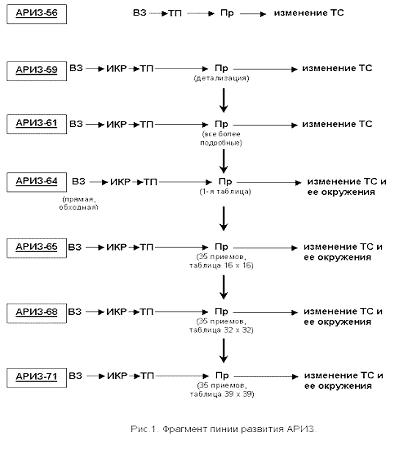
\includegraphics[width=.7\textwidth]{./8.jpg}
\end{center}

Ю.П. Саламатов \cite{Salamatov1992} также считал, что Таблица появилась уже в
АРИЗ-64. В составленной им линии развития АРИЗ она упоминается в составе
АРИЗ-64 как «1-я таблица» из четырех, правда, без указания числа приемов
(Рис. 1).

Но в АРИЗ-64, опубликованном Официальным Фондом Г.С. Альтшуллера (выдержка из
книги \cite{Altshuller1964}), работа с Таблицей технических противоречий, как
составляющая часть шагов оперативной стадии, не упоминается.  Да и в конспекте
«История развития АРИЗ» \cite{Altshuller1986a}, говоря об АРИЗ-64, Альтшуллер
упоминает о ней, скорее, мимоходом: «\textbf{Впервые} составлена таблица
\textbf{групп приемов}».  Он даже не считает ее \textbf{первой} Таблицей, --
\textbf{первая} появляется, по его мнению, лишь в АРИЗ-65.

Можно лишь предположить, что последователи Генриха Сауловича «обобществили»
АРИЗ-64 с материалами его книги, в которой эта версия алгоритма была изложена.
Ведь даже понятие технического противоречия в АРИЗ-64 встречается лишь однажды
-- в первом шаге оперативной стадии: «Проверить возможность устранения
технического противоречия изменением данного объекта (машины, механизма,
процесса)».  Таблицы же в нем нет и в помине.

Группа специалистов из ТРИЗЛАБ (Ideation TRIZLAB of the International TRIZ
Associa\-tion), в составе которой сразу три Мастера ТРИЗ, «свернула» историю
создания Таблицы радикально: 
\begin{quote}
  Таблица и приемы были созданы в 1971 году и явились одним из первых
  эффективных инструментов
  ТРИЗ»\footnote{\url{http://www.trizscientific.com/TRIZ_sci/history/history09_recomend_r.htm}
    -- no more online. HGG}.
\end{quote}
При этом отмечены основные заслуги автора:
\begin{quote}
  Альтшуллер внес двойной вклад в развитие рекомендаций для изобретателя:
  \begin{itemize}
  \item Основал рекомендации (приемы) не на субъективном опыте изобретателей,
    а на анализе патентного фонда (к уровню объективности этой процедуры нам
    еще предстоит вернуться -- Л.Ш.).
  \item Перешел от одномерной структуры предъявления приемов (список) к
    двухмерной (таблица технических противоречий), позволяющей более
    эффективно отыскивать нужные рекомендации.
  \end{itemize}
\end{quote}
Столь же браво обошлись Мастера ТРИЗ-Лаб и с историей
АРИЗ\footnote{\url{http://www.trizscientific.com/TRIZ_sci/history/history06_ariz_r.htm}
  -- no more online. HGG}.  Явное противоречие в указаниях даты рождения
Таблицы, размещенных на соседних страницах сайта, их, по-видимому, ничуть не
смутило:
\begin{quote}  
  1959 Первый вариант краткого алгоритма (без названия «алгоритм) в первой
  опубликованной статье по ТРИЗ

  1960 \textbf{Появление названия «Алгоритм изобретения»} и 5 шагового
  циклического алгоритма

  1964 ARIZ-64

  1969 \textbf{ARIZ-69 с таблицей приемов разрешения технических противоречий} 

  1971 ARIZ-71 с физическим противоречием
\end{quote}
Сравним выделенные строки с конспектом Г.С.Альтшуллера «История развития
АРИЗ»:
\begin{quote}  
  АРИЗ-65. \textbf{Введена первая (еще очень небольшая) таблица устранения
    технических противоречий}. Оперативная часть по-прежнему включает анализ
  природных прототипов. \textbf{Впервые появилось слово «алгоритм»} -- как
  указание на дальнюю цель развития программы». \cite{Altshuller1986a}
\end{quote}
Итак, по мнению Альтшуллера, первая Таблица была введена в АРИЗ-65. Что же
было до нее? Становится очевидным, что «История развития АРИЗ» (и Таблицы как
одной из его составляющих) далеко не так однозначна, как кажется. И
разобраться в ней -- дело не такое уж простое.

На сайте ТРИЗ-Лаб говорится и о том, что еще в конце 80-х года было
предпринято 
\begin{quote}
  несколько неудачных попыток разработки новых версий ARIZ -- Королева,
  Андриевского, Ладошкина и других. Г. Альтшуллер возражал против того, чтобы
  кто-то кроме него разрабатывал версии АРИЗ, так как АРИЗ является его
  авторским
  материалом\footnote{\url{http://www.trizscientific.com/TRIZ_sci/history/history06_ariz_r.htm}
    -- no more online. HGG}.
\end{quote}
Но прошло несколько лет, и 
\begin{quote}
  в 1989 Альтшуллер официально разрешил разработку «не альтшуллеровских»
  версий алгоритма. Тогда же состоялось совещание с участием Зусман, Злотина,
  Злотиной, Литвина, Петрова по разработке новой версии ARIZ.
\end{quote}

Противоречивые и (как в дальнейшем нетрудно будет заметить) зачастую неверные
версии «Новой истории ТРИЗ» не только мешают постичь логику развития методики
и ее основного логического механизма -- АРИЗ, но и ее «главного» (по частоте
применения) на сегодняшний день инструмента -- Таблицы. Учитывая уже
упоминавшиеся в первой статье особенности формирования авторского коллектива
на начальных стадиях, они лишают нас возможности понять и оценить вклад того
или иного соавтора в развитие АРИЗ и его частей. Интересно понять, что же
происходило на самом деле, как складывалась «история развития ТРИЗ».
Реализуемо ли это при таком значительном различии мнений?

Ответ на этот вопрос предложил сам Г.С. Альтшуллер. В перечне ходов ЖСТЛ
\cite{Altshuller1994} в разделе Постэндшпиль дается недвусмысленная
рекомендация (№ 84) реакции на ход внешних обстоятельств. «Искажение истории»:
Ход творческой личности -- «Использование архивного материала». В целях
постепенного и неуклонного формирования в себе качеств творческой личности,
будем стараться максимально использовать открытые публикации, доступные
архивные материалы и свидетельства.

Общее число рабочих вариантов Таблицы достоверно не известно. Выборочный опрос
Мастеров ТРИЗ показал, что таковых могло быть от одного до четырех. Впрочем,
мало (очень-очень мало) кто из Мастеров готов перечислить даже три варианта.
Так что этот вопрос вполне можно использовать на экзаменах в качестве
«завального». Впрочем, это и не удивительно. Несмотря на самоотверженную
работу Фонда ГСА по опубликованию работ и ЧОУНБЭ -- по их сбору, классификации
и предоставлению рабочих материалов, в общедоступном виде (например, в
Интернете) находятся, действительно, лишь два-три варианта. На первый взгляд,
может показаться несущественным то значение, которое придается здесь времени
включения Таблицы в АРИЗ. В действительности, с учетом дополнительных
сведений, почерпнутых из «второстепенных» источников, это обстоятельство имеет
особый, и, как будет показано в дальнейшем, важный смысл.

«Раскопки» в архивах, проведенные при подготовке этой статьи, показали, что за
относительно короткий период своего роста и преобразования Таблица имела не
менее шести разновидностей, пять из которых опубликованы. И лишь три варианта
включались самим Альтшуллером в качестве составных частей в Алгоритмы Решения
Изобретательских Задач: АРИЗ-65 (16 параметров / 35 приемов), АРИЗ-68 (32/35)
и АРИЗ-71 (39/40). Возможно, что некоторые «зародышевые» и промежуточные
варианты просто затерялись или забылись в повседневной борьбе за продвижение
основных идей ТРИЗ. Все же представляется важным выделить в них хотя бы
основные отличия, позволяющие проследить логику развития и видоизменения этого
главного инструмента тризного зарубежья.

\subsection*{Ты помнишь, как все начиналось?}

В 1992 году Ю.П. Саламатов отметил, что «в ТРИЗ осталось множество белых
пятен, неисследованных и недостаточно понятых проблем и разделов»
\cite{Salamatov1992}. Возможно, он и не был первым, кто это заметил. Но он был
первым, кто сделал это мастерски. Освещая в своей работе «самые серьезные
исследования по ИМ-ТРИЗ-технологии», Саламатов сделал особое ударение на том,
что 
\begin{quote}
  в ходе этих работ идет интенсивная проверка степени разработанности,
  истинности, зрелости всех разделов ТРИЗ -- базы знаний новых компьютерных
  систем. Вскрываются новые пласты теории, по-новому представляются некоторые
  разделы, четко проявляются недостатки, недоработки, становятся видными
  перспективы развития теории изобретательства.
\end{quote}
\textbf{Разработанность, истинность, зрелость!} -- Здорово сказано!  Красиво.

Но, отслеживая вехи становления и преобразования «железной леди», так и тянет
спросить: «А кто же все-таки помнит, как все начиналось?» Но спросить не у
кого. Вот о том, как возникали стандарты, можно спросить у Мастера ТРИЗ
В. Петрова. О «диверсионке» -- у Мастера ТРИЗ Б. Злотина. О справочнике
физэффектов у Мастера ТРИЗ Ю. Горина. Об АРИЗ когда-то можно было спросить у
Кандидата в Мастера ТРИЗ Р. Шапиро. А про ЭТО?

На соавторство или хотя бы на сопереживание в создании Таблицы, похоже, никто
и никогда всерьез не претендовал. Ею от начала и до конца занимался только
Альтшуллер, и именно \textbf{его} последний вариант, ценит и безоговорочно
принимаемый всем тризным и околотризным миром, канонизирован и причислен к
лику святых. В чем секрет этого признания? В том ли, что в Таблице все так
фантастически просто? Или в том, что история ее создания, как и стоящая за нею
технология, практически никому неизвестны? Элементарность ли заполняющих
Таблицу счастливых номеров завораживают новичков ТРИЗ, или непостижимая даже
для самого смелого воображения необозримость океана переработанной информации,
словно гипнотизируя, заставляет даже видавших виды Мастеров вновь и вновь
полагаться на удачу в ТРИЗном Лото?

В опубликованной в 1961 году в книге «Как научиться изобретать»
\cite{Altshuller1961} АРИЗ-61 («улучшенная модификация АРИЗ-59«) новые
разработки уживались со старыми проблемами. «Расширена оперативная часть. Но
правил выполнения шагов по-прежнему нет» \cite{Altshuller1986a}. Расширение
произошло за счет развертывания уже имевшихся трех шагов и введения четвертой
группы -- списка из четырех приемов, проверяющих возможности разделения
объекта на независимые части. Именно эти четыре группы, включающие 20 приемов,
были условно сведены в тексте книги в первую, пока еще виртуальную таблицу
будущего: 
\begin{quote}
  Изобретателю полезно иметь таблицу таких приемов и постоянно ее пополнять,
  приглядываясь к методам решения различных технических задач. В качестве
  основы для таблицы могут послужить четыре группы приемов, с которыми мы уже
  познакомились. При пополнении таблицы \textbf{можно не заботиться о
    строгости классификации. Достаточно, чтобы приемы располагались от
    простого к более сложным}. Когда техническое противоречие выявлено,
  изобретатель должен, не полагаясь на память, взять лист с таблицей приемов и
  последовательно проверить пригодность каждого приема. Проверить без спешки,
  не отдавая заранее предпочтения тому или иному приему, не пропуская приемы,
  кажущиеся «заведомо непригодными». Очень часто лучшее решение дают именно
  эти заведомо непригодные приемы.
\end{quote}

Поскольку «улучшение» в АРИЗ-61 по сравнению с АРИЗ-59 носило пока еще
значительно более выраженный количественный, чем качественный характер (хотя
будущий переход количества в качество и наметился), авторами этой
«модификации», по-прежнему следовало бы считать дуэт Альтшуллер-Шапиро. Ведь,
как уже отмечалось, «Шапиро проработал в ТРИЗ по 1961-й год». Ну, добавилась
еще одна группа? Ну, появились еще четыре приема? По сути-то обе модификации
идентичны. Правда, немного смущают даты. Было ли расширение оперативной части
и распад дуэта в 1961 году простым совпадением? Проработал Шапиро «в ТРИЗ» по
1961-й год -- только до появления новой группы приемов, или он ушел уже после
этого?

В 1961 году была издана книга Шапиро \cite{Bachmatov1961}. Судя по тому, что и
книга Альтшуллера была издана в том же году, а ее подготовка и написание
заняли, возможно, не один месяц, отход Шапиро от совместной работы произошел
уже после или во время введения в АРИЗ новой группы приемов. Могло ли иметь
столь малозначительное, на первый взгляд, расширение оперативной стадии АРИЗ
какое-то отношение к его решению? А может быть, четвертая группа приемов
именно потому и смогла войти в АРИЗ-61, что Шапиро уже не хотел или не был в
состоянии этому помешать? Ведь он был единственным, кто мог противиться
механистическому расширению АРИЗ.

Ответы на эти и многие другие вопросы, возможно, будут найдены в личных
архивах основоположников ТРИЗ, в их переписке, набросках и черновиках.
Остается надеяться, что тризное движение достигнет в обозримом будущем такого
размаха, при котором подобные «раскопки» начнут представлять интерес и для
широкой общественности.

Сравнительный анализ ранних вариантов алгоритма показывает, что в них
«табличные» свойства присущи группам приемов лишь в зачаточном состоянии
(1.-4. шаги оперативной стадии) -- к преобразованию в какой-либо механизм,
например, сведению в Таблицу, они еще совершенно не были готовы. Причин тому
видится несколько. В первую очередь, это отсутствие правил выполнения шагов в
целом и чересчур общее, абстрактное определение части из них (в особенности, в
составе третьего и четвертого шагов).

Вот эти группы, без особых ухищрений представленные в виде шагов оперативной
стадии АРИЗ-61:

\textbf{Первый шаг.} Проверка возможных изменений в самом объекте (т. е. в
данной машине, данном технологическом процессе).
\begin{itemize}
\item[1.] Изменение размеров.
\item[2.] Изменение формы.
\item[3.] Изменение материала.
\item[4.] Изменение температуры.
\item[5.] Изменение давления.
\item[6.] Изменение скорости.
\item[7.] Изменение окраски.
\item[8.] Изменение взаимного расположения частей.
\item[9.] Изменение режима работы частей с целью максимальной их нагрузки.
\end{itemize}
\textbf{Второй шаг.} Проверка возможности разделения объекта на независимые
части.
\begin{itemize}
\item[1.] Выделение «слабой» части.
\item[2.] Выделение «необходимой и достаточной» части.
\item[3.] Разделение объекта на одинаковые части.
\item[4.] Разделение объекта на разные по функции части.
\end{itemize}
\textbf{Третий шаг.} Проверка возможных изменений во внешней (для данного
объекта) среде.
\begin{itemize}
\item[1.] Изменение параметров среды.
\item[2.] Замена среды.
\item[3.] Разделение среды на несколько частичных сред.
\item[4.] Использование внешней среды для выполнения полезных функций.
\end{itemize}
\textbf{Четвертый шаг.} Проверка возможных изменений в соседних
(т.е. работающих совместно с данным) объектах.
\begin{itemize}
\item[1.] Установление взаимосвязи между ранее независимыми объектами,
  участвующими в выполнении одной работы.
\item[2.] Устранение одного объекта за счет передачи его функций другому
  объекту.
\item[3.] Увеличение числа объектов, одновременно действующих на ограниченной
  площади, за счет использования свободной обратной стороны этой площади.
\end{itemize}

Несмотря на расширение, оперативная стадия АРИЗ-61 все еще мало чем отличалась
от классического списка контрольных вопросов. Как и в АРИЗ-56, а затем и в
АРИЗ-59, «Оперативная часть сходна с синектикой -- расчет на аналогию (прежде
всего -- на использование природных прототипов)» \cite{Altshuller1986a}.
Введение «разделительных» приемов, действительно отличающихся технической
новизной, лишь указало на возможности дальнейшего увеличения списка, но вовсе
не сделало «третью по счёту версию гораздо 'алгоритмичней'«, как это пытается
представить автор будущей Энциклопедии ТРИЗ \cite{Korolyev1998}.

Правило распределения приемов в будущей Таблице (и, следовательно, порядок их
применения), сводящееся к их расположению «от простого к более сложным» должно
было увеличивать эффективность перебора вариантов, повышая вероятность
нахождения удачного приема еще до завершения полного просмотра всех групп. Но
перебор вариантов как таковой (а, следовательно, и МПиО в целом) это решение
еще вовсе не исключало. Возможно, именно неразработанность механизма
применения приемов, их бросающаяся в глаза неалгоритмичность служили причиной
того, что приемам еще не придавалось первостепенного значения в развитии АРИЗ.
Во всяком случае, имелись серьезные затруднения в определении этого значения.
А ведь именно на приемах и «прообразах» была выстроена практически вся
оперативная стадия (см. приведенный выше фрагмент АРИЗ-61) и, как следствие,
именно на них ложилась основная ответственность за успешное применение АРИЗ.
Эти обстоятельства и вынуждали Альтшуллера производить регулярную перепись
приемов, чтобы нащупать в них скрытые закономерности и попытаться их
«приручить». Прежде всего, это требовалось затем, чтобы «развернув» шаги
оперативной стадии, вывести приемы -- хотя бы визуально -- из опасной зоны
действия МПиО.

Появление собственно развернутых групп (списков) приемов фактически произошло
уже в АРИЗ-59 -- в первых трех шагах оперативной стадии (ОС), только здесь они
еще не были пронумерованы. Альтшуллер и Шапиро отказались от термина «прием»
при поиске решений в системе, надсистемах и внешней среде (подшаги второго
шага, перенесенные в начало оперативной стадии), заменив его на «возможные
изменения». А «типичные приемы (прообразы)» решения в природе и технике были
окончательно переименованы в «прообразы» и, таким образом, формально лишены
статуса «приемов». В АРИЗ-61 произошло лишь одно принципиальное изменение --
добавление во втором шаге ОС четвертой (с учетом «прообразов» -- шестой)
группы специальных приемов, узко направленных на «проверку возможности
разделения объекта на независимые части».

Те же пять групп приемов, составлявшие оперативную стадию (в неразвернутом,
тезисном виде), присутствовали и в самом первом пра-алгоритме -- АРИЗ-56
\cite{Altshuller1956}:
\begin{itemize}
\item[1.] Исследование типичных приемов решения (прообразов):
  \begin{itemize}
  \item[а)] в природе,
  \item[б)] в технике.
  \end{itemize}
\item[2.] Поиски новых приемов решения путем изменений:
  \begin{itemize}
  \item[а)] в пределах системы,
  \item[б)] во внешней среде,
  \item[в)] в сопредельных системах.
  \end{itemize}
\end{itemize}
Оперативная стадия АРИЗ-59 отличалась от предложенного в статье 1956 перечня
шагов лишь некоторой их детализацией. Кроме того, изменилась
последовательность шагов: «Поиски новых приемов путем изменений» переместились
на первое место, сдвинув «Исследование типичных приемов решения (прообразов)»
в конец стадии. Зато в АРИЗ-61 году произошел своеобразный прорыв в развитии
структуры оперативной стадии. Введение на втором шаге пока еще небольшой
группы новых приемов на «выделение части» и «разделение на части» открывало
новые перспективы для расширения до тех пор еще обозримого списка подшагов.
Перечень «изменяющих приемов» не просто увеличился на 4 пункта, но
«развернулся» и был значительно детализирован, приняв форму списка проверочных
рекомендаций из 20 отдельных приемов. В большинстве своем (первый и второй
шаги) эти приемы носили уже вполне прикладной характер, который еще нагляднее
подчеркивался новыми приемами:
\begin{quote}
  Второй шаг. Проверка возможности разделения объекта на независимые части.
  \begin{itemize}
  \item[1.] Выделение «слабой» части.
  \item[2.] Выделение «необходимой и достаточной» части.
  \item[3.] Разделение объекта на одинаковые части.
  \item[4.] Разделение объекта на разные по функции части.
  \end{itemize}
\end{quote}

Все 20 приемов в АРИЗ-59 по-прежнему носили общий, универсальный и
ненаправленный характер, как по отношению к будущему решению, так и по
отношению к исходной изобретательской ситуации. Это обстоятельство и вынуждало
применять их при поиске решения, как и в 1956-м, «в последовательности от
простого к сложному, что позволяло получить правильные решения с минимальной
затратой усилий и времени». Рекомендации авторов были фактически излишни,
отражая лишь объективную слабость приемов и неизбежную необходимость их
перебора. Применение приемов в очередности, соответствующей убыванию их
простоты и частоты употребления, обещало, на первый взгляд, некоторое
повышения вероятности нахождения «правильного решения» еще до окончания всего
списка.

Однако с ростом числа приемов все более заметно стало обостряться новое
противоречие. Как не раз отмечалось, 
\begin{quote}
  Сами приемы не несут в себе конкретных решений. Увидеть решение, развернуть
  его на основе предлагаемого принципа или подсказки должен сам решающий
  задачу. Поэтому работа с каждым приемом не может быть простой и быстрой. На
  прием надо настроиться, внимательно и скрупулезно просмотреть возможности
  использования заложенных в нем рекомендаций под самыми разными углами
  зрения. Даже в самом экономном, ускоренном режиме работа с одним приемом
  занимает в процессе реального решения задач не менее получаса.
  \cite{Kudryavtsev}
\end{quote}

Иными словами, регулярное применение 16 приемов в 1959 году занимало в
процессе решения задачи от 4 до 8 часов интенсивной групповой или
индивидуальной работы. Введение же четвертой группы приемов, определившее
новое направление развития АРИЗ, ставило их комплексное применение под угрозу
невыполнимости. Непомерные затраты времени на перебор уже имевшихся приемов
воздвигали мощный барьер перед соблазнительной перспективой дальнейшего
расширения списка. Но самой значительной проблемой по-прежнему оставалось их
ненаправленное применение.

Используя столь любимую Альтшуллером практику аналогий, применение приемов
можно было представить как стрельбу из лука по кучевым облакам
изобретательской ситуации, возможно, содержащим в себе нужные идеи для
«правильного решения». Стрелами являлись приемы -- каждый со своим порядковым
номером и определенными свойствами. «Правильное решение», как предполагалось,
крылось где-то в облаке изобретательской ситуации. Решателю предлагалось
поупражняться в стрельбе из лука, стараясь попасть в его невидимый центр -- в
надежде вызвать выпадение благодатного «дождя» идей, устраняющего противоречие
на пути к ИКР (Рис. 2).

\begin{center}
  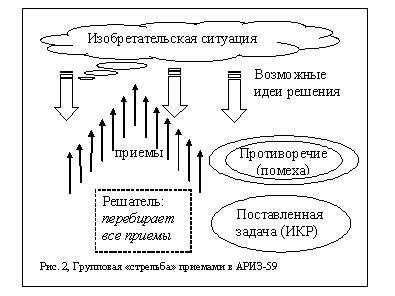
\includegraphics[width=.7\textwidth]{./9.jpg}
\end{center}

При этом не было ясно, откуда нужно стрелять и какое направление выбирать.
Занять ли для стрельбы постоянную позицию или передвигаться от выстрела к
выстрелу, но куда? Стрелять в центр облака или в самое «темное» его место?
Ясно было лишь одно: Желательно воспользоваться всеми стрелами по очереди.
Поэтому все стрелы-приемы запускались (каждым решателем в отдельности) из
одной точки и летели в одном и том же направлении (а порой и в одно место): От
решателя, с его субъективным видением приемов, прямо в «облако»
изобретательской ситуации.

Как следствие, получение одной из возможных идей решения поставленной задачи
(идеального результата) являлось скорее функцией удачливости и опыта,
накопленного решателем, чем объективной силы предлагаемых приемов. Неизбежно
возникала парадоксальная ситуация, при которой объективно полезное сужение
постановки задачи приводило к снижению вероятности результативного попадания
каждым из приемов (использование которых оставалось, несмотря на имеющиеся
примеры, делом крайне субъективным) в отдельности. В особенно невыгодное
положение ставило это обстоятельство начинающих решателей.

Необходимость перебора всех вариантов, ненаправленность действия приемов,
субъективность выбора последовательности их применения, снижение вероятности
результативного попадания в результате сужения постановки задачи -- все это
снижало привлекательность работы на оперативной стадии, так же как и
эффективность алгоритма в целом. Нестабильность на оперативном участке АРИЗ
неизбежно отражалась и недоверием к его работоспособности, причем не только у
новичков. Первой попыткой конструктивного решения этих проблем стало
объединение в 1964 году накопленных приемов в «таблицу групп приемов», которую
Альтшуллер подробно описал в своей новой книге «Основы изобретательства»
\cite{Altshuller1964}, но не решился официально включить в состав алгоритма.
\clearpage

\begin{flushright}
  «Чтоб музыкантом быть, так надобно уменье…«\\
  (И.А. Крылов, Квартет)
\end{flushright}
\section*{4. Впервые составленная таблица групп приемов}

Как уже отмечалось, внешний вид, форма и структура Таблицы на разных этапах ее
становления не только соответствовали ее реальному внутреннему содержанию,
объемам и качеству переработанной при ее подготовке информации или
возможностям практического применения, но и отражали развитие представлений
авторов о ее функциях. Вернее, автора. Ведь Таблица (то есть собственно
числовая матрица) является уникальным явлением и, возможно, единственным
атрибутом ТРИЗ, по отношению к которому допустимо было утверждать -- по
крайней мере, до сих пор, -- что идея его создания, его разработка,
преобразования и отладка принадлежат Альтшуллеру, только Альтшуллеру и никому
другому.

Следовательно, допустимо было бы также предположить, что именно на примере
Таблицы и связанным с нею изменениям в АРИЗ последователям Генриха Сауловича
предоставляется редкая возможность проследить изменение его представлений о
ТРИЗ на значительном отрезке времени.

В изданной в 1961 году первой книге Г.С. Альтшуллера «Как научиться
изобретать» \cite{Altshuller1961} Таблицы как таковой мы не находим.
Следовательно, допустимо утверждать, что в 1961 году ее еще не существовало.
Зато приемам и их применению отведено немало места в главах, посвященных
примерам разбора задач по АРИЗ: 
\begin{quote}
  Поиски ведутся по определенной рациональной системе. Общей формулы нет, но
  есть приемы, достаточные для большинства случаев. Изобретателю нужно
  систематически перепробовать эти приемы. Как правило, один из них дает
  искомое решение.
\end{quote}

Очевидно, что только весьма ограниченное число приемов позволяло автору
рекомендовать решателям фактически Метод Проб и Ошибок, чтобы «систематически
перепробовать эти приемы». «Максимум нового эффекта при минимуме затрат на
реализацию -- такова формула хорошего изобретения», -- этот призыв Альтшуллера
в не меньшей степени относился и к самому творческому процессу. Минимум затрат
на поиск нужного приема при максимально успешном результате, -- так можно было
бы сформулировать новую стратегическую цель развития ТРИЗ на ближайшие годы.

Первой (во всяком случае, первой официально зарегистрированной в работах
Г.С. Альтшуллера) попыткой конструктивного решения проблем, связанных с
использованием приемов, стало их объединение в 1964 году в «таблицу групп
приемов». Альтшуллер подробно описал эту таблицу в своей второй книге «Основы
изобретательства» \cite{Altshuller1964}, но из-за обстоятельств, остающихся
пока еще малопонятными, не стал включать в состав алгоритма.

\subsection*{Не выплеснуть ребенка с грязной водой…}

Насколько тернистым и нескорым мог быть путь к новой идее, можно представить,
вспомнив высказывание Альтшуллера: 
\begin{quote}
  Когда техническое противоречие выявлено, изобретатель должен, не полагаясь
  на память, взять лист с таблицей приемов и последовательно проверить
  пригодность каждого приема. Проверить без спешки, не отдавая заранее
  предпочтения тому или иному приему, не пропуская приемы, кажущиеся «заведомо
  непригодными». Очень часто лучшее решение дают именно эти заведомо
  непригодные приемы \cite{Altshuller1961}.
\end{quote}

Конечно, в 1961 число приемов было еще невелико. И таблице, описанной в книге,
пока еще не отводилась роль панацеи в деле устранения технических
противоречий. Ее задачей было лишь немного упорядочить их применение, «не
заботясь о строгости классификации». Собственно, и таблицей предлагаемый
список можно было называть лишь условно -- по признаку делимости приемов на
тематические группы.

«Достаточно, чтобы приемы располагались от простого к более сложным»,
утверждал автор. На вопрос о том, что именно подразумевалось под простотой или
сложностью приемов, читатель не получал однозначного ответа. Но, судя по тем
примерам, которыми были снабжены отдельные приемы, можно было сделать
определенные предположения. «Простыми» следовало считать приемы, более или
менее стабильно и быстро узнаваемые самим автором в новых технических решениях
и задачах.

Возможно, не отдавая себе отчета в важности сделанного заявления, Альтшуллер
отверг саму возможность создания реального механизма, способного обеспечить
объективный выбор наиболее подходящих приемов. Ведь чем точнее и изощреннее
был бы этот инструмент, чем больше «заведомо непригодных» приемов удавалось бы
отсеять с его помощью уже на подготовительной стадии работы, тем выше
становилась бы вероятность потери «лучших решений».

Да уж. Такому противоречию не были бы рады и опытные тризовцы наших дней. Но…
Альтшуллер или не заметил его остроты, или сделал вид, что не заметил. Так или
иначе, он интенсивно разрабатывал, разыскивал, придумывал и заимствовал все
новые и новые приемы. Мысль о том, что таким образом он увеличивает и число
«заведомо непригодных» приемов, отсеять которые с каждым расширением списка
становится все труднее и рискованнее, Генриха Сауловича пока еще всерьез не
тревожила.

ТРИЗ проскочила исторический разъезд на полном ходу, и машинист не заметил,
что путевая стрелка направила его в тупик. Эффективный механизм выбора
«правильных приемов», как идеальная, но недостижима цель, остался где-то в
стороне.

Оглядываться на расставляемые собственными руками логические капканы и ловушки
было некогда: АРИЗ «расширялся», Альтшуллер экспериментировал, зарождались
новые, давно уже «назревшие» инструменты, наглядно свидетельствующие о
планомерном развитии всей методики. Новой оригинальной разработке суждено
обернуться действенным инструментом, позволяющим АРИЗ оправдать и свое
название, и высокое предназначение.

\subsection*{Лирическое отступление}

В предыдущей статье отмечалось, что одной из причин низкой эффективности при
использовании приемов была низкая «прицельность стрельбы». Уровень
объективности использования приемов определялся и оценивался самим решателем.
Отсутствовала определенность при выборе исходной позиции. Неопределенность в
работе с приемами осложняла восприятие решателем логики оперативной стадии,
тормозила развитие АРИЗ и всей методики в целом.

Но, в первую очередь, «страдали» сами приемы.

Этот эффект знаком любому преподавателю, хоть раз включавшему Таблицу в
программу своих семинаров. За первыми восторгами от успешного применения
приемов при решении учебных задач следуют уже менее убедительные подходы
преподавателя к решению производственных задач слушателей. А затем наступает
неизбежная развязка. После нескольких попыток самостоятельного использования
табличного инструментария на практике, доверие к нему у большинства слушателей
семинаров заметно снижается. Ни блестящая эрудиция лектора, ни эффектные и
убедительные примеры зачастую не могут преодолеть той беспомощности, которую
испытывают начинающие тризовцы, оставаясь один на один с реальной задачей.

В том, что вот уже третье поколение преподавателей ТРИЗ великолепно, быстро и
безошибочно -- да что уж скромничать, просто блестяще решает \textbf{Учебные
  Задачи}, заслуга в значительной степени «основоположников» методики. Большая
часть решений таких задач, ставших классикой ТРИЗ, -- это значительно
упрощенные, на первый взгляд методические разборы их поэтапного решения,
ретроспективно «притянутые за уши» к нескольким блестящим идеям. Ни
всеобъемлющего описания проблемной ситуации, ни заблуждений и уводящих в
сторону заманчивых линий развития, которые неизбежно присутствуют в каждом
реальном проекте, ни строгой логики в анализе результата учащиеся в этих
примерах, как правило, не находят.

Поиск решений, которых во всякой реальной ситуации (в отличие от «учебной«)
всегда несоизмеримо больше, неизбежно ведется на многоуровневой основе. При
этом использование приемов, если такое вообще допустимо, способно как-то
оживить этот поиск только для простейших минимальных задач развития, до
которых ой как не просто докопаться. Тому, кто на это способен, приемы
становятся практически не нужны.

Сказать об этом компетентно смогли бы сегодня, в лучшем случае, два-три
десятка решателей. Но в открытую поднимать эту тему считается неприличным.
Абсолютно честного, подробного и полного «конспекта» серьезного ТРИЗ-проекта,
начинающегося с постановки задачи заказчиком и заканчивающегося внедрением
полученной концепции решений в производство, встречать пока еще не
приходилось. А свернутый в десяток страниц успешный «экспресс»-анализ способен
убедить только новичков или профанов.

Немудрено, что большинство тризовцев, долгое время специализирующихся на
преподавании основ методики, привносят в свою будущую практическую
деятельность элементы шапкозакидательства. Мол, сейчас «вколем» пару
приемчиков -- и все пройдет.

Особенно ярко проявляется эта тенденция у «новых тризовцев» на Западе, где
роль упаковки при продаже любого товара давно уже играет существенную, если не
определяющую роль. А истоки такого наполеоновского отношения к любым проблемам
лежат «у колыбели» ТРИЗ. Ведь сам «методический подход» начался с выделения
«готовых» приемов на основании описаний изобретений, и, следовательно, с
неизбежной (хотя и не всегда осознанной) примитивизации всех возможных проблем
в области техники и технологии производства.

В тех же основополагающих заблуждениях 50-х годов следует искать и корни
другого, когда-то воспринимавшегося причудливым и школярским, а теперь уже
модного и весьма прибыльного направления в развитии ТРИЗ. Речь идет о
повальном применении приемов, закодированных в Таблицу, во всех без исключения
отраслях человеческой деятельности. Можно было бы предоставить приемлемость
такого подхода совести ее апологетов вроде Дерелла Манна, сумевшего создать
целую индустрию наподобие Fast-TRIZ\footnote{Перечень его наиболее
  значительных «табличных» работ можно найти здесь:
  \url{https://triz-journal.com/?s=matrix}}.

Но продолжать замалчивать опасность, которую такого рода деятельность
представляет для ТРИЗного движения в целом, о необратимом загрязнении пока еще
восприимчивой к ТРИЗ мировой предпринимательской среды было бы
безответственным.

Остается лишь воспользоваться тем удачным стечением обстоятельств, что давно
не живешь в своем отечестве, чтобы немного попророчествовать: собрав первый
урожай с еще непуганых «русской методикой» просторов, «табличные» дельцы рано
или поздно уйдут со сцены. Жаль, что чистые воды ТРИЗ ожидает участь Байкала.
Зато будет больше бумаги.

Хорошо, что уже после нас.

\subsection*{И ноты есть у нас, и инструменты есть}

«Приемы -- инструменты в творческой мастерской изобретателя. А в хорошей
мастерской инструменты никогда не лежат, как попало. Поэтому на оперативной
стадии творческого процесса приемы должны использоваться по определенной
системе», настаивал Учитель \cite{Altshuller1961}. Но тот порядок, в котором
он раскладывал собранные им инструменты в своей изобретательской «анатомичке»,
далеко не всегда помогал другим пользователям при операциях на «живых»
проблемах.

Таблица и укрытые под ее сенью приемы являются не только слабым звеном ТРИЗ,
но и одним из наиболее запутанных сюжетов в ее истории.

\begin{quote}
  При отработке методики были испытаны различные последовательности
  расположения этих приемов. Наиболее целесообразной представляется такая
  система, при которой приемы устранения технических противоречий расположены
  от простых и наиболее часто употребляемых к сложным и сравнительно редко
  употребляемым \cite{Altshuller1961}.
\end{quote}

При всем уважении к усилиям автора книги по перекладыванию приемов и
перетасовке их в различных комбинациях, приходится признать, что поиски
решения велись «неконвенциональными» для ТРИЗ, попросту обратными
пропагандируемым методами. Как и то, что уровень «лучшего решения» был, мягко
говоря, далек от идеального.

Следя за превращениями оперативной стадии АРИЗ в период между 1956 и 1964
годом, невольно вспоминаешь «музыкальную» басню. Попытки авторов методики
взять власть над приемами в свои руки сводились, в основном, к чисто
организационным мероприятиям. «Оркестр» то расширялся, то «сворачивался».
«Музыкантов» пересаживали из одной группы в другую. Заменялись или
преобразовывались «оркестровые инструменты». Но музыки -- стабильной,
эффективной, быстродействующей системы выбора подходящих приемов для получения
«лучших решений» -- так и не было слышно.

Смирившись с тем, что состав списка приемов будет постоянно изменяться как в
количественном, так и в качественном отношении (а с такими темпами
«дополнений», как в 1961 году, работы могло хватить на десятилетия),
Альтшуллер изменил тактику. По-прежнему расширяя Список, он вплотную приступил
к исходной «суперзадаче», названной еще в 1956 году. А именно, к созданию
универсальной системы выбора подходящего приема. То есть такой системы,
которая исправно работала бы в любых изменяющихся условиях, с \textbf{любым
  составом приемов}.

О том, как, когда и у кого родилась спасительная идея, Альтшуллер не упоминал.
Он лишь прямо указывал наиболее волнующую его в АРИЗ-61 проблему:

«Расширена оперативная часть. \textbf{Но правил выполнения шагов по-прежнему
  нет}» \cite{Altshuller1986a}. Под правилами выполнения шагов подразумевались
основные условия выбора и применения приемов. «По-прежнему», -- значит,
проблема волновала его и раньше. Но не решалась.

Пока еще призрачная надежда возлагалась теперь на то, что из посредственных
музыкантов сможет получиться дружный оркестр. Не доставало лишь одного --
строгого дирижера.

Пусть сами приемы субъективны и неоднозначны как в их трактовке, так и в их
применении. Пусть эффективность их использования в значительной степени
зависит от образования, опыта и мировоззрения пользователя. Но если придать их
использованию закономерный характер? Если разработать строгие правила,
основывающиеся на более или менее объективных параметрах и свойствах самой
изобретательской ситуации, объекта изобретения?

Так начался новый эксперимент. И имя ему -- ТАБЛИЦА.

Что вынуждало Альтшуллера почти два десятилетия так отчаянно бороться за
приемы? С методической точки зрения интересным более важным представляется то,
как он это делал.

К цели он шел, применяя им же разработанные методы, учитывая собственные
рекомендации, введенные им во вновь организованную стадию АРИЗ-64 «Уточнение
формулировки задачи»:
\begin{quote}
  Проверить, можно ли достичь той же цели решением «обходной» задачи.
  Определить, решение какой задачи -- первоначальной или «обходной» -- может
  дать больший эффект.
\end{quote}

В типовых приемах недостатка больше не было (списки постоянно уточнялись). А
вот вплотную подойти к выделению «типовых противоречий» до сих пор не
удавалось. И главное, неясной оставалась будущая логическая связка,
позволяющая безошибочно находить для каждого «типового противоречия» свой --
типовой же -- прием.

Так возникла «обходная» задача, выглядевшая более привлекательно. Требовалось
смоделировать логическую связку между типовыми ухудшающимися характеристиками,
типовыми противоречиями и типовыми приемами, позволяющую безошибочно находить
для каждого «типового противоречия» свой -- типовой же -- прием.

«Обходная» задача сулила несравнимо большую эффектность от применения приемов.

Скажи лишь, как нам сесть!

В качестве исходных позиций для «стрельбы» приемами впервые были выбраны
«недопустимые ухудшения» параметров известных ТС. Десять таких характеристик
(в порядке возрастания от А до К) были положены в основу будущей Таблицы:
\begin{itemize}
\item[А)] Недопустимое увеличение веса объекта
\item[Б)] Недопустимое увеличение длины объекта
\item[В)] Недопустимое увеличение площади объекта
\item[Г)] Недопустимое увеличение объема
\item[Д)] Недопустимое изменение формы
\item[Е)] Недопустимое повышение требуемой мощности (или энергии)
\item[Ж)] Недопустимое снижение надежности
\item[З)] Недопустимое снижение производительности
\item[И)] Противоречивое сочетание требований к условиям работы объекта
\item[К)] Возникновение вредных факторов, например, вредных сил
\end{itemize}
Понятие Технического Противоречия (ТП) было еще слабо развито. Уже
одностороннее ухудшение одного из рабочих параметров ТС представлялось
необходимым и достаточным условием для возникновения Технического
Противоречия, пригодного для «обстрела» приемами.

Это представление немедленно выразилось в радикальном преобразовании первого
шага оперативной стадии:
\begin{quote}
  «Проверить возможность устранения технического противоречия изменением
  данного объекта».
\end{quote}
Под «изменением» подразумевался результат активного применения одного из
изобретательских принципов, объединяющих приемы в семь различных по составу и
силе групп.
\begin{itemize}
\item[] Количественные изменения
\item[] Изменение условий работы объекта
\item[] Разделение объекта
\item[] Принцип совмещения
\item[] Компенсация нежелательных факторов
\item[] Принцип «наоборот»
\item[] Принцип «динамизации» объектов
\end{itemize}
Изменилось и указание цели для «стрельбы приемами» на пятом шаге аналитической
стадии. До сих пор в АРИЗ-59 и АРИЗ-61 оно формулировалось слишком уж обще и
больше походило на указание того, во что стрелять не надо:
\begin{quote}
  Определить, при каких условиях не мешало бы (то есть найти условия, при
  которых противоречие снимается).
\end{quote}
В АРИЗ-64 это положение получило не только принципиально новую форму, но и
несравненно более конкретное содержание:
\begin{quote}
  Определить, при каких условиях \textbf{ничто} не мешало бы получить
  \textbf{идеальный результат} (ответить на вопрос: «При каких условиях
  исчезнет «помеха»?).
\end{quote}
Правда, сам автор считал главным достижением этой версии АРИЗ изменение его
начальной стадии:
\begin{quote}  
  Введение новой части -- «проверка и уточнение условий задачи». Это
  принципиальное изменение: взят курс на развитие АРИЗ как инструмента для
  сильного решения трудных задач \cite{Altshuller1986a}.
\end{quote}
Но все же, с учетом интенсивных разработок Таблиц в 1965/68/71 годах, «светом
в конце туннеля» представляется именно новая, лишь начинающая прорисовываться
система в выборе и применении приемов:
\begin{quote}
  \textbf{Впервые появляется правило выполнения шагов} (на шаге 2.1):
  Проверить возможность устранения технического противоречия изменением
  данного объекта (машины, механизма, процесса).
\end{quote}
Вместе с нею первые появился и шанс на создание реально управляемого процесса,
повышающего прицельность «стрельбы» приемами. Самое же главное, -- процесс
этот постепенно наряжался в пока еще легкие и прозрачные одежды объективности.

Приемы обретали характер (или, во всяком случае, признаки) векторов, основания
которых были привязаны к известным, недопустимо ухудшающимся характеристикам,
а направление определял ИКР (Рис. 1) Задачей приемов стало устранение «помехи»
на пути к ИКР. Предполагаемая эффективность от их применения должна была при
этом повыситься. Как и убедительность всего преподаваемого на семинарах по
ТРИЗ материала, связанного с приемами.
\begin{center}
  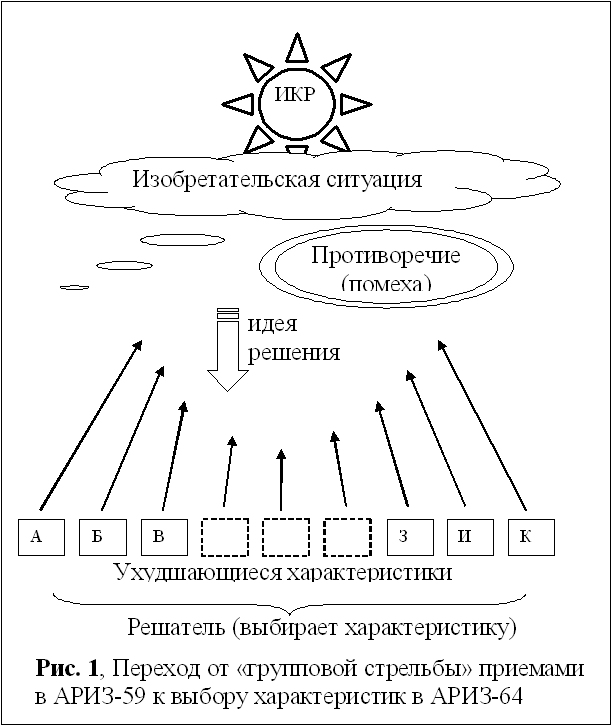
\includegraphics[width=.7\textwidth]{./16.jpg}
\end{center}

Все это должно было способствовать укреплению веры в работоспособность приемов
у пользователей. Правда, произошло значительное понижение их статуса:

Из «\textbf{Решателей, перебирающих по очереди все приемы}», пользователи АРИЗ
опускались до ранга «\textbf{Решателей, выбирающих ухудшаемые
  характеристики}».  По крайней мере, визуально.

В основу нового инструмента был заложен стандартный психологический эффект: С
введением предварительного отсева приемов ответственность Решателя за их выбор
(вернее, за правильный перебор) резко снижалась. Теперь забота о выборе
приемов как бы перешла в прошлое надсистемы (АРИЗ и его автор), стала решаться
«заранее». Она перекладывалась на Составителя Таблицы, недвусмысленно
гарантирующего успех при использовании лишь ограниченного числа приемов,
связанных с ухудшающейся характеристикой. Соответственно должна была
многократно возрастать вера в успешность «избранной» группы приемов. Они
попросту не могли не срабатывать. Не имели права.

О том, что в 1961 году Альтшуллер рекомендовал составление индивидуальной
таблицы каждому пользователю, предпочиталось больше не напоминать.

Каким именно образом автор Таблицы подбирал те или иные приемы, было его
собственным Know-how. Это уже не должно было волновать Решателя, который
отныне мог спокойно сконцентрироваться на более тщательном обдумывании лишь
нескольких табличных «избранников». Значительная важность придавалась теперь
«правильному определению» ухудшающейся характеристикой. Именно в сторону этого
решения перемещался центр тяжести будущей улучшенной оперативной стадии.

Раньше использование приемов напоминало Сизифов труд, узаконенный в последнем
шаге оперативной стадии АРИЗ-59 и АРИЗ-61:
\begin{quote}
  Возвращение (в случае непригодности всех рассмотренных приемов) к исходной
  задаче и расширение ее условий, т. е. переход к другой, более общей задаче.
\end{quote}
Иными словами, Решатель обязывался перебирать все приемы «до победного конца»
или до полного поражения. И неоднократно, если понадобится.

Общее число приемов возросло против 1961 года в несколько раз. Перебирать их
стало невозможно уже исходя из основных принципов борьбы с МПиО. Но с приходом
Таблицы эта необходимость отпадала сама собой. Зато относительная
«прицельность» использования каждого из приемов в отдельности повысилась
многократно.

Но самым, пожалуй, важным качеством будущего инструмента -- с точки зрения
адаптации методики к производственным условиям -- становилось значительное
снижение затрат времени на прохождение части оперативной стадии, связанной с
«упорядоченными» приемами. Прежний страх перед тем, что, несмотря на высокую
стоимость анализа (как уже упоминалось, при 16 приемах он составлял от 4-х до
8-ми часов рабочего времени), он может завершиться неудачей, отступал.
Утомительная и напряженная процедура прохождения «приемной» стадии теперь
превращалась в приятную тренировку ума и сообразительности на час-полтора, не
более.

\subsection*{Облегчение оперативной стадии}

Плоская иллюстрированная матрица, явившаяся первой документально
подтвержденной графической попыткой Альтшуллера упорядочить применение
собранных к тому времени изобретательских принципов, получила двойное
название:

В приложении к книге она была озаглавлена «\textbf{Основные приемы устранения
  технических противоречий}» (Рис. 2).

\begin{center}
  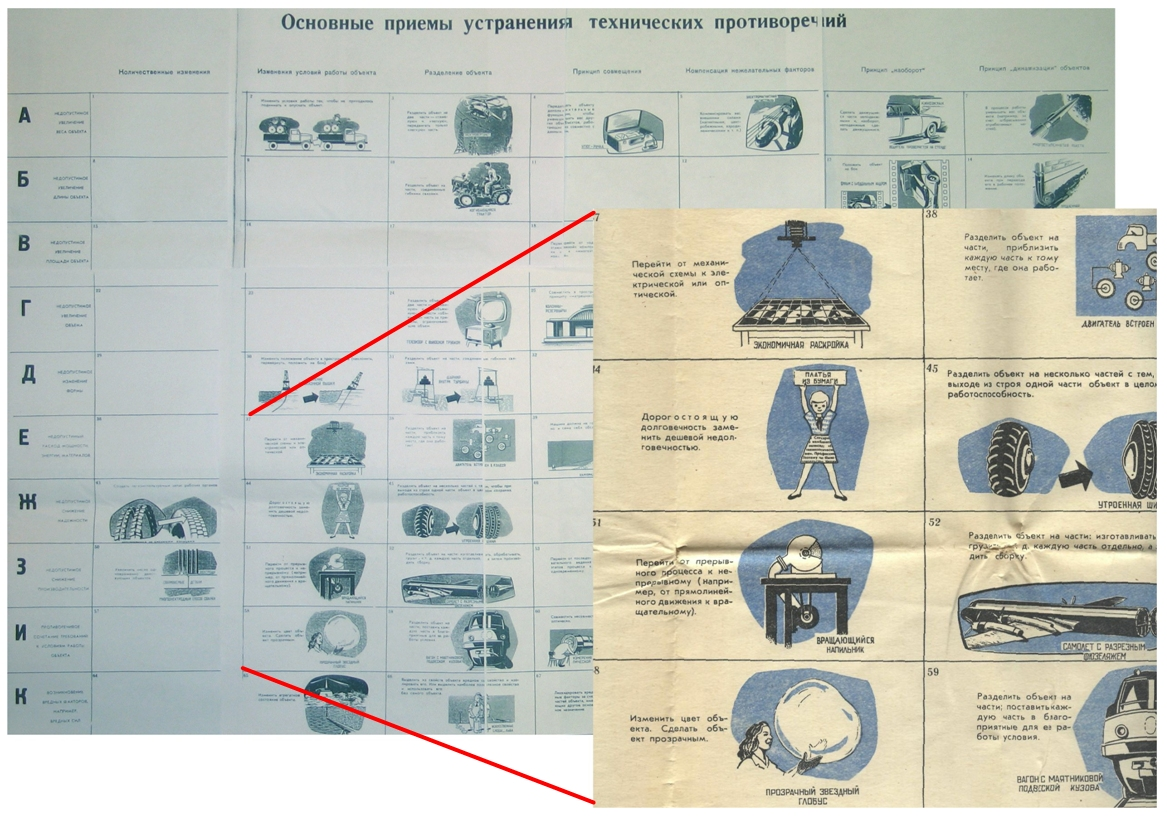
\includegraphics[width=.7\textwidth]{./17.jpg}\\
  Рис. 2 Основные приемы устранения технических противоречий.
\end{center}

В более поздних разъяснениях к истории развития АРИЗ сам Альтшуллер называл ее
«\textbf{Впервые составленной таблицей групп приемов}» \cite{Altshuller1986a}.

Возможно, именно благодаря этому разночтению позднее распространилось
убеждение в том, что «первая Таблица» была введена уже в АРИЗ-64.

Она еще не предлагала готовые наборы приемов для различных конфликтующих пар.
Да и понятие «конфликтная пара» для работы с нею еще не требовалось. В ней
демонстрировались лишь принципиальные возможности применения отдельных приемов
для \textbf{устранения} «помехи» -- недопустимого ухудшения одной из десяти
сформулированных технических характеристик. Оставалось неясным и то, что же
подразумевалось под этим -- предотвращение, компенсация, преобразование или
какой-то другой вид \textbf{устранения} технических противоречий.

Собственно техническое противоречие в его привычной для нас сегодня двойной
форме, таким образом, здесь еще не формулировалось, а лишь подразумевалось.
Выбор приема осуществлялся «скрещиванием» в Таблице исходной ухудшаемой
характеристики с основными изобретательскими принципами.

В отличие от трех своих последовательниц, эта Таблица была, скорее, первой
пробой пера. Но вопрос о ее включении в АРИЗ представлялся практически
решенным:
\begin{quote}
  Таблица предназначена для того, чтобы \textbf{облегчить оперативную стадию
    творческого процесса}. Анализ выявляет помеху, то есть присущее задаче
  техническое противоречие. После этого надо обратиться к таблице и проверить
  возможность устранения помехи приемами, указанными в соответствующем
  горизонтальном ряду. \cite{Altshuller1964}
\end{quote}
Все же избранный подход оставался кустарным и недостаточно убедительным:
\begin{quote}  
  Помните, что типовые приемы сформулированы в общем виде. Конкретное же
  противоречие, с которым вы будете сталкиваться при решении задач, имеет
  индивидуальные особенности. Типовые приемы подобны готовому платью. Их надо
  подогнать, учитывая индивидуальные особенности, индивидуальные требования.
\end{quote}
В чем именно выражалась и во что выливалась «подгонка готового платья», так и
осталось неизвестным.

Принципиальная возможность использования всех возможных вариантов не
исключалась, но заполненными были только 40 полей из 70 возможных. Сам
Альтшуллер объяснял такое избирательное заполнение клеток нежеланием
перегружать Таблицу приемами второстепенного значения:
\begin{quote}  
  Некоторые из них оставлены незаполненными. Можно, конечно, сформулировать
  приемы и для этих клеток. Но тогда типовые сильные приемы затеряются среди
  \textbf{слабых} приемов, \textbf{редко} используемых на практике.
\end{quote}
Зато каждый указанный прием сопровождался примером, снабженным отдельным
рисунком:
\begin{quote}  
  Типовые приемы проиллюстрированы в таблице конкретными примерами.
  Разумеется, каждый пример поясняет лишь часть той общей идеи, к которой он
  относится. Примеры говорят о наглядных, но конкретных случаях. В то время
  как \textbf{каждый прием отображает общий принцип}.
\end{quote}
Впрочем, Альтшуллер и не скрывал того, что использование приемов на практике
является скорее искусством (может быть, даже Великим Искусством), чем легко
изучаемым ремеслом:
\begin{quote}  
  Мастерство изобретателя на этом этапе работы заключается в умении гибко
  пользоваться идеями, содержащимися в общих формулах приемов.
\end{quote}
Наиболее перспективным -- по числу выявленных их применений -- представлялся
принцип «Разделение объекта» (тот самый шаг-выскочка, лишь недавно
«проклюнувшийся» в АРИЗ-61 с четырьмя новыми приемами). В девяти случаях из
десяти возможных этот принцип позволял устранять «помеху» (недопустимое
ухудшение технической характеристики) на пути к ИКР.

А вот «Количественные изменения», большие надежды на которые возлагались еще в
первых вариантах АРИЗ, помогали теперь только в двух случаях. В последующих
Списках и Таблицах этот принцип уже не встречался, а использованные для него
ранее примеры (Рис. 3) можно было легко перераспределить между другими
приемами. В том, что уже на основании рисунков к примерам каждый начинающий
тризовец найдет им новые применения, сомневаться не приходится.
\begin{center}
  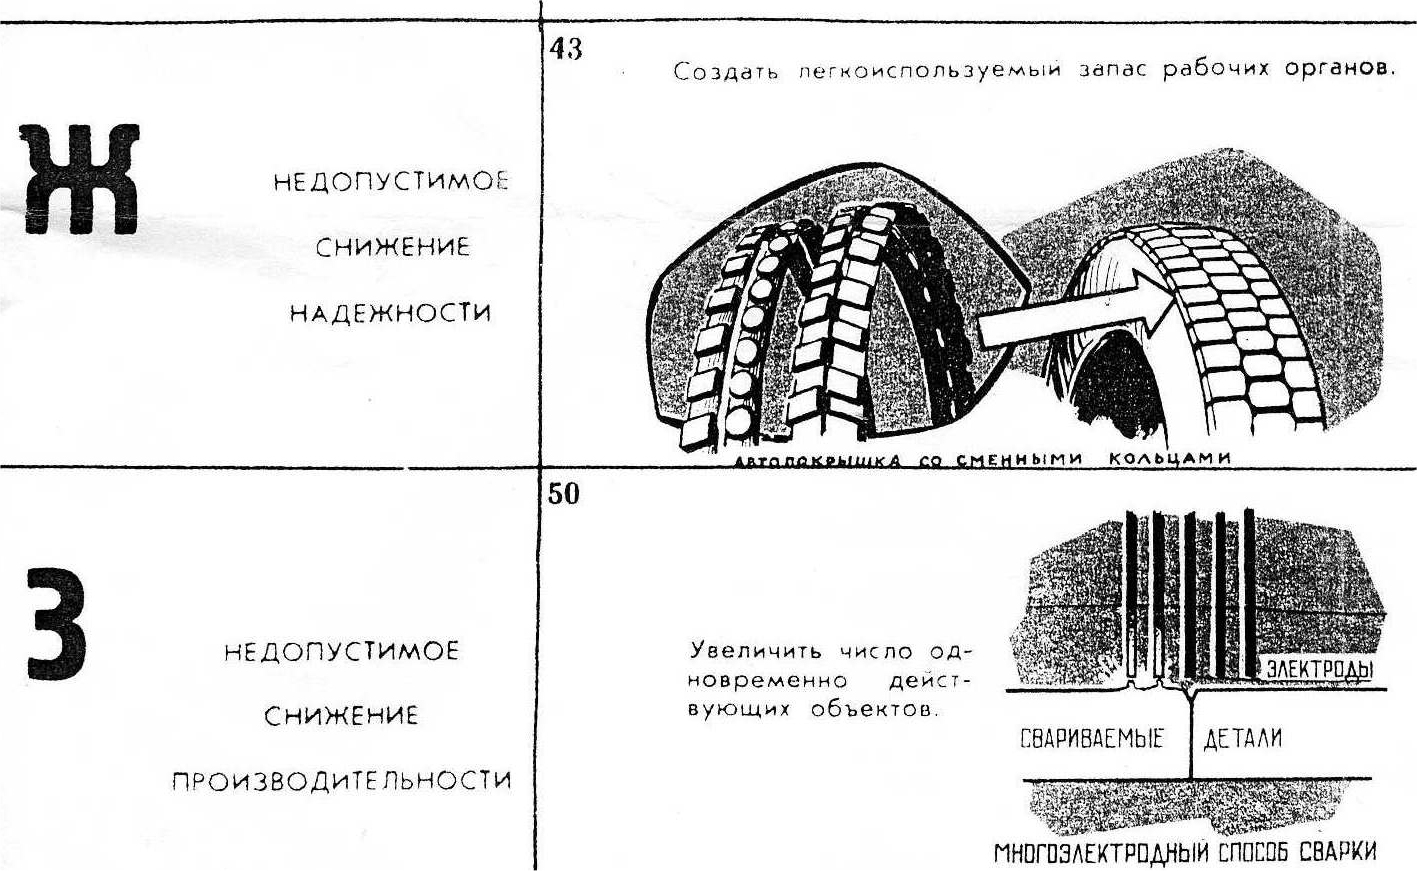
\includegraphics[width=.8\textwidth]{./18.jpg}\\
  Рис. 3. Приемы из «утерянного колена» -- Количественные изменения
\end{center}

Возможно, именно несовершенство первой «таблицы групп приемов» явилось
причиной того, что Альтшуллер воздержался от непосредственного включения ее в
АРИЗ-64.  Как и того, что сам автор о ней позднее почти не упоминал.

\subsection*{Немного статистики}

Объемы статистических данных, легших в основу первой Таблицы Альтшуллера,
достоверно не известны. Можно лишь сослаться на выдержку из статьи 1959 года:
\begin{quote}  
  Найти эти закономерности было нелегко. Мы искали их в истории техники, в
  описаниях сотен, тысяч изобретений, в воспоминаниях великих изобретателей, а
  главное -- \textbf{в огромном опыте, накопленном советскими новаторами}.
  \cite{Altshuller1959}
\end{quote}
Более конкретные цифры появились в книге «Как научиться изобретать»
\cite{Altshuller1961}: 
\begin{quote}
  Работа над созданием такой методики была начата мною в 1946 году. …  Уже в
  первые три года работы (то есть за время до первого ареста Альтшуллера и
  Шапиро -- Л.Ш.) были проанализированы 4\,000 описаний различных изобретений.
\end{quote}

Если исходная база данных для «впервые составленной таблицы групп приемов»
достоверно неизвестна, то можно провести анализ ее самой. Весьма поучительной
представляется приведенная ниже сравнительная таблица.

В ней перечислены приемы в составе шагов АРИЗ-61 и Способы устранения ТП в
Таблице-1964. Жирным шрифтом здесь выделены те приемы, которые в той или иной
форме перешли в состав Таблицы из АРИЗ-61. Или хотя бы узнаются в ней.

Подчеркиванием\footnote{Changed to asterisk added -- HGG} выделены группы
приемов, «свернутые» в АРИЗ-64 в первый шаг (информационную базу Таблицы).
Неподчеркнутыми представлены группы приемов, оставшиеся в АРИЗ-64 формально
самостоятельными.

Казалось бы, в Таблице-1964 мы должны встретить все тринадцать приемов из
первых двух групп АРИЗ-61. Объединенные теперь в первом шаге АРИЗ-64, они
должны были составить, в результате объединения шагов, информационную базу
Таблицы. Но таких приемов оказалось лишь восемь.

Пять приемов из первых двух групп АРИЗ-61 (выделены курсивом) исчезли целиком
и полностью. «Потерялись» три приема на изменение -- материала, температуры,
давления. \emph{Выделение «необходимой и достаточной» части}, как и
\emph{Разделение объекта на одинаковые части} тоже потеряли свою актуальность
и в Таблицу не вошли.  Зато в нее добавились сразу тридцать два (32!) большей
частью принципиально новых Способа устранения ТП.

\begin{center}
  \begin{tabular}{|p{.35\textwidth}|p{.35\textwidth}|p{.15\textwidth}|}\hline
    \multicolumn{3}{|c|}{Сравнительная таблица приемов (1961) и Способов
      устранения ТП (1964)} \\\hline
    Приемы в составе шагов АРИЗ-61& Способы устранения ТП в Таблице-1964&
Номер клетки (способа)\\\hline
Изменение размеров$^\ast$ & Изменить условия работы так, чтобы не поднимать и не
опускать объект.& 2\\\hline
Изменение формы$^\ast$& Разделить объект на две части -- «тяжелую» и «легкую»,
передвигать только «легкую» часть.& 3\\\hline
\emph{Изменение материала} & Передать объекту дополнительные функции, чтобы
уменьшить вес других объектов, работающих совместно с данным. & 4\\\hline
\emph{Изменение температуры} & Компенсировать вес внешними силами (магнитными,
центробежными, аэродинамическими и т.п.). & 5\\\hline
\emph{Изменение давления} & Сделать движущиеся части неподвижными и, наоборот,
неподвижные -- движущимися. & 6\\\hline
Изменение скорости$^\ast$  & Уменьшить -- в процессе работы -- вес объекта
(например, за счет отбрасывания отработанных частей). & 7\\\hline
Изменение окраски$^\ast$  & Разделить объект на части, соединенные гибкими
связями. & 10 \\\hline
Изменение взаимного расположения частей$^\ast$ & Положить объект на бок (+) & 
13\\\hline
Изменение режима работы частей с целью максимальной их нагрузки$^\ast$  &
\textbf{Изменить длину объекта при переводе его в рабочее положение}. &
14\\\hline 
Выделение «слабой» части  & \textbf{Перейти от «одноэтажной» компоновки к
«многоэтажной«}. & 18\\\hline
\emph{Выделение «необходимой и достаточной» части} & Изменять в процессе работы
площадь объекта. & 21\\\hline
\emph{Разделение объекта на одинаковые части} & \textbf{Разделить объект на
  две части -- «объемную» и «необъемную». Вывести «объемную» часть за пределы,
  ограничивающие объем}. & 24\\\hline
  \end{tabular}

  \begin{tabular}{|p{.35\textwidth}|p{.35\textwidth}|p{.15\textwidth}|}\hline
Разделение объекта на разные по функции части$^\ast$ & Совместить в пространстве
несколько объемов (принцип «матрёшки«). & 25\\\hline
Изменение параметров среды & Изменить объем при переводе объекта в рабочее
положение & 28\\\hline
Замена среды & Изменить положение объекта в пространстве (наклонить,
перевернуть, \textbf{положить на бок}) (+) & 30\\\hline
Разделение среды на несколько частичных сред & Разделить объект на части,
соединенные гибкими связями. & 31\\\hline
Использование внешней среды для выполнения полезных функций & \textbf{Создать 
предварительное изменение формы, противоположное недопустимому}. & 33\\\hline
Установление взаимосвязи между ранее независимыми объектами, участвующими в
выполнении одной работы. & \textbf{Выполнить объект из материала, допускающего 
изменение формы при работе}. & 34\\\hline
Устранение одного объекта за счет передачи его функций другому объекту. &
Выполнить объект из материала, допускающего изменение формы при работе. &
35\\\hline
Увеличение числа объектов, одновременно действующих на ограниченной площади,
за счет использования свободной обратной стороны этой площади. & Перейти от
механической схемы к электрической или оптической. & 37\\\hline
&Разделить объект на части, приблизить каждую часть к тому месту, где она
работает. &38\\\hline
&Машина должна не только выполнять основную работу, но и сама себя
обслуживать. &39\\\hline
&\textbf{Компенсировать расход энергии получением какого-либо дополнительного
  эффекта}. &40\\\hline
&\textbf{Перейти от непрерывной подачи мощности к периодической, например,
  импульсной}. &42\\\hline
&Создать легко используемый «запас» рабочих органов. & 43\\\hline
&Дорогостоящую долговечность заменить дешевой недолговечностью. & 44\\\hline
  \end{tabular}

  \begin{tabular}{|p{.35\textwidth}|p{.35\textwidth}|p{.15\textwidth}|}\hline
&\textbf{Разделить рабочий орган на несколько частей с тем, чтобы, при выходе
      из строя одной части, объект в целом сохранял работоспособность}.  &
    45\\\hline
&Увеличить число одновременно действующих объектов.  & 50\\\hline
&Перейти от прерывного процесса к непрерывному (например, от прямолинейного
движения к вращательному). & 51\\\hline
&Разделить объект на части; изготовлять каждую часть отдельно, затем
производить сборку. & 52\\\hline
&Перейти от последовательного ведения этапов процесса к одновременному. &
53\\\hline
&\textbf{Изменить цвет объекта. Сделать объект прозрачным}. & 58\\\hline
&\textbf{Разделить объект на части: поставить каждую часть в благоприятные для
  ее работы условия}. & 59\\\hline
&Совместить несовместимое оптически.& 60\\\hline
&Объект должен менять свои свойства при изменении условий работы.& 63\\\hline
&Изменить агрегатное состояние объекта.& 65\\\hline
&Выделить из свойств объекта вредное свойство и изолировать его. Или выделить
наиболее полезное свойство и использовать его без самого объекта. & 66\\\hline
&Ликвидировать вредные факторы за счет частей объекта, имеющих другое основное
назначение.& 67\\\hline
  \end{tabular}

  \begin{tabular}{|p{.35\textwidth}|p{.35\textwidth}|p{.15\textwidth}|}\hline
&Компенсировать вредные факторы за счет самих этих факторов (клин клином).
Использовать вредные факторы для выполнения полезной работы. & 68\\\hline
&Усилить вредные факторы настолько, чтобы они перестали быть вредными. &
69\\\hline
  \end{tabular}
\end{center}

Таким образом, общее число Способов устранения технического противоречия во
«впервые составленной Таблице групп приемов» 1964 года составило ровно сорок.

Это число поначалу сбивает с толку. Ведь сегодня известно, что все 40 типовых
приемов появились впервые в Таблице образца 1971 года.

Тщательное сравнение Способов устранения ТП в Таблице-1964 со списком 40
типовых приемов Таблицы в АРИЗ-71 не оставляет сомнения в простом совпадении
чисел: В Таблице-1964 в той или иной степени «проявляются» (с учетом здоровой
доли субъективности автора статьи) только 26 «классических» типовых приемов,
приведенных ниже в порядке возрастания номеров:

\paragraph{«Классические» типовые приемы, узнаваемые в Таблице-1964 как
  Способы устранения технических противоречий}
\begin{itemize}
\item[1.] Принцип дробления
\item[2.] Принцип вынесения
\item[3.] Принцип местного качества
\item[6.] Принцип универсальности
\item[7.] Принцип «матрешки«
\item[8.] Принцип антивеса
\item[9.] Принцип предварительного антидействия
\item[12.] Принцип эквипотенциальности
\item[13.] Принцип «наоборот«
\item[15.] Принцип динамичности
\item[16.] Принцип частичного или избыточного действия
\item[17.] Принцип перехода в другое измерение
\item[19.] Принцип периодического действия
\item[20.] Принцип непрерывности полезного действия
\item[21.] Принцип проскока
\item[22.] Принцип «обратить вред в пользу«
\item[23.] Принцип обратной связи
\item[25.] Принцип самообслуживания
\item[26.] Принцип копирования
\item[30.] Использование гибких оболочек и тонких пленок
\item[32.] Принцип изменения окраски
\item[35.] Принцип изменения агрегатного состояния
\end{itemize}

Несколько смущает только одно обстоятельство. Работа эта велась в
несвойственной для Альтшуллера атмосфере секретности; Информация о
промежуточных результатах или источниках получения новых приемов не
встречается в публикациях Генриха Сауловича 1961--1963 годов.

\subsection*{АРИЗ подстраивается под Таблицу}

Ограниченные возможности полосы не дают возможности провести сравнение всех
ранних версий АРИЗ. Поэтому попытаемся провести сравнительный анализ только
основных его «дотабличных» вариантов. Для удобства сравнения одинаковые
смысловые шаги в них расположены на одном уровне\footnote{Due to editorial
  issues we provide the columns of the table in succession indicating the row
  numbers for each entry. Note that ARIZ-64 has entries extended over several
  rows.}

\paragraph{АРИЗ-59 \cite{Altshuller1959}}
\begin{itemize}
\item[(1)] \textbf{Оперативная Стадия} (Устранение условий, вызывающих причину
  технического противоречия путем внесения изменений в одну из частей машины.)
\item[(2)] \textbf{Первый шаг}. Проверка возможных изменений в самом объекте
  (то есть в данной машине, данном технологическом процессе и т. д.):
  изменение размеров, числа частей, формы, взаимосвязи частей, материала,
  температуры, давления, скорости и т. д.
\item[(3)] x
\item[(4)] \textbf{Второй шаг}. Проверка возможных изменений во внешней среде:
  изменение параметров среды, замена среды, использование среды для выполнения
  полезных функций.
\item[(5)] \textbf{Третий шаг}. Проверка возможных изменений в других
  (соседних для данного) объектах: установление взаимосвязи с соседними
  объектами, изменение характера ранее установленной взаимосвязи, отказ от
  соседнего объекта за счет переложения его функций на данный объект.
\item[(6)] \textbf{Четвертый шаг}. Исследование прообразов из других отраслей
  техники (поставить вопрос: Как данное противоречие устраняется в других
  отраслях техники?)
\item[(7)] x
\item[(8)] \textbf{Пятый шаг}. Исследование прообразов в природе (поставить
  вопрос: Как данное противоречие устраняется в природе?)
\item[(9)] \textbf{Шестой шаг}. Возвращение (в случае непригодности всех
  рассмотренных приемов) к исходной задаче и расширение ее условий, то есть
  переход к другой, более общей задаче.
\end{itemize}
\paragraph{АРИЗ-61 \cite{Altshuller1961}}
\begin{itemize}
\item[(1)] \textbf{Оперативная Стадия}
\item[(2)] Проверка возможных изменений в самом объекте (т. е. в данной
  машине, данном технологическом процессе).
  \begin{enumerate}
  \item Изменение размеров.
  \item Изменение формы.
  \item Изменение материала.
  \item Изменение температуры.
  \item Изменение давления.
  \item Изменение скорости.
  \item Изменение окраски.
  \item Изменение взаимного расположения частей.
  \item Изменение режима работы частей с целью максимальной их нагрузки.
\end{enumerate}
\item[(3)] \textbf{Второй шаг}. Проверка возможности разделения объекта на
  независимые части.
  \begin{enumerate}
  \item Выделение «слабой» части.
  \item Выделение «необходимой и достаточной» части.
  \item Разделение объекта на одинаковые части.
  \item Разделение объекта на разные по функции части.
  \end{enumerate}
\item[(4)] \textbf{Третий шаг}. Проверка возможных изменений во внешней (для
  данного объекта) среде.
  \begin{enumerate}
  \item Изменение параметров среды.
  \item Замена среды.
  \item Разделение среды на несколько частичных сред.
  \item Использование внешней среды для выполнения полезных функций.
\end{enumerate}
\item[(5)] \textbf{Четвертый шаг}. Проверка возможных изменений в соседних
  (т.е. работающих совместно с данным) объектах.
  \begin{enumerate}
  \item Установление взаимосвязи между ранее независимыми объектами,
    участвующими в выполнении одной работы.
  \item Устранение одного объекта за счет передачи его функций другому
    объекту.
  \item Увеличение числа объектов, одновременно действующих на ограниченной
    площади, за счет использования свободной обратной стороны этой площади.
  \end{enumerate}
\item[(6)] \textbf{Пятый шаг}. Исследование прообразов из других отраслей
  техники (поставить вопрос: Как данное противоречие устраняется в других
  отраслях техники?).
\item[(7)] x 
\item[(8)] \textbf{Шестой шаг}. Исследование прообразов в природе (поставить
  вопрос: Как данное противоречие устраняется в природе?).
\item[(9)] \textbf{Седьмой шаг}. Возвращение (в случае непригодности всех
  рассмотренных приемов) к исходной задаче и расширение ее условий, т.е.
  переход к другой, более общей задаче.
\end{itemize}

\paragraph{АРИЗ-64 \cite{Altshuller1964}} 
\begin{itemize}
\item[(1)] \textbf{Оперативная Стадия}
\item[(2-3)] \textbf{Первый шаг}: Проверить возможность \textbf{устранения
  технического противоречия изменением данного объекта} (машины, механизма,
  процесса).
\item[(4-5)] \textbf{Второй шаг}: Проверить возможные изменения в среде,
  окружающей объект, \textbf{и в других объектах, работающих совместно с
    данным}.
\item[(6)] \textbf{Третий шаг}: Перенести решение из других отраслей техники
  (ответить на вопрос: Как решаются в других отраслях техники задачи, подобные
  данной?).
\item[(7)] \textbf{Четвертый шаг}: Применить «обратные» решения (ответить на
  вопрос: Как решаются в технике задачи, обратные данной, и нельзя ли
  использовать эти решения, взяв их, так сказать, со знаком минус?).
\item[(8)] \textbf{Пятый шаг}: Использовать «прообразы» природы (ответить на
  вопрос: Как решаются в природе более или менее сходные задачи?).
\item[(9)] x
\end{itemize}

Уже отмечалось, что в АРИЗ-64 произошло вынесение первого шага аналитической
стадии и образование отдельной стадии -- «Уточнение формулировки задачи».

Наряду с этим, в АРИЗ-64 произошли и другие преобразования, так или иначе
связанные с предстоящим введением Таблицы непосредственно в алгоритм. В
значительной степени эти изменения определили и будущую политику развития
ТРИЗ.

\textbf{Во-первых}, в оперативной стадии последовало бесследное и, на первый
взгляд, парадоксальное исчезновение лишь недавно введенного в АРИЗ-61 второго
шага вместе со всей группой «разделительных» приемов.

Вместо него появился новый четвертый шаг оперативной стадии:
\begin{quote}\it  
  Применить «обратные» решения (ответить на вопрос: «Как решаются в технике
  задачи, обратные данной, и нельзя ли использовать эти решения, взяв их, так
  сказать, со знаком минус?«).
\end{quote}
Этот шаг (пусть пока обще сформулированный) продолжил традицию поэтапного
расширения АРИЗ за счет вновь наработанных приемов. За ним стояла новая, еще
неразвернутая группа приемов с общей «философией«: Сделай наоборот!

Выделение \emph{«обратных»} решений в отдельный логический шаг было не
случайным. Как и выделение второго, \emph{«разделительного»} шага в АРИЗ-61.
Это еще больше подчеркнуло новизну и большой потенциал заложенных в новых
шагах приемов.

Но периоды независимости новых групп приемов оставались недолгими. Так же как
пропал из оперативной стадии «разделительный» шаг, суждено было и
«наоборот«-шагу вскоре исчезнуть. Не успев «развернуться», он занял место в
конце первого шага вновь созданной стадии «Уточнение условий задачи» в
АРИЗ-68.

А свое «выставочное» место в оперативной стадии «наоборот«-шаг уступил в
АРИЗ-68 следующей группе приемов. Очередным фаворитом стал четвертый шаг:

\emph{Проверка возможных изменений во времени}.

\textbf{Второе} значительное изменение, отличающее АРИЗ-64 от его
предшественников, выразилось в исчезновении последнего, седьмого шага
оперативной стадии, до этого исправно работавшего в АРИЗ-59 и АРИЗ-61:
\begin{quote}\it  
  Возвращение (в случае непригодности всех рассмотренных приемов) к исходной
  задаче и расширение ее условий, т.е. переход к другой, более общей задаче.
\end{quote}
За этой не слишком обидной пропажей крылся, однако, поистине политический
манифест: \textbf{Отбросить все сомнения! Оперативная стадия обязана решать
  любую задачу!}

Что же придало автору алгоритма такую безусловную уверенность? Что позволило
ему утверждать, что уже одноразовый проход по оперативной стадии (с
использованием всех предлагаемых приемов) будет достаточным для успешного
решения любой поставленной задачи? Что до \emph{возвращения к исходной задаче
  и расширение ее условий, т. е. переход к другой, более общей задаче} дело
уже не дойдет?

Возможных ответов представляется несколько (с учетов вновь введенного
«уточнения формулировки задачи«):
\begin{enumerate}
\item Альтшуллер обнаружил неисчерпаемый источник новых приемов, покрывающих
  все разнообразие известных технических решений, из которого он мог
  долговременно пополнять, расширять, обновлять и уточнять как «табличный»
  Список, так и АРИЗ.
\item Разрастание Списка приемов подтолкнуло его к идее о постепенном
  перераспределении приемов между различными «инструментами«: Таблицей,
  независимыми шагами оперативной стадии и начинавшимися разрабатываться
  операторами (по сути, «мини-оперативными стадиями» целевого назначения). Это
  позволяло значительно дольше и интенсивнее «играться» с различными приемами,
  не особенно рискуя оказаться в роли простого «переборщика вариантов».
\item Ему удалось «нащупать» идею нового механизма -- оператора для снятия
  психологической инерции, позволяющего создать у решателя ощущение
  ускоренного выбора наиболее удачных приемов из постоянно расширяющегося
  списка. Одновременно у решателя снижался страх ответственности за возможную
  неудачу.
\end{enumerate}

\textbf{В третьих}, в АРИЗ-64 произошло не только радикальное «сворачивание»
трех совсем недавно «развернутых» групп приемов, но и пока еще трудно
объяснимое объединение двух из них в лаконичный второй шаг:
\begin{quote}
  Проверить возможные изменения в среде, окружающей объект (3-й шаг в АРИЗ-61
  -- Л.Ш.), и в других объектах, работающих совместно с данным (4-й шаг в
  АРИЗ-61 -- Л.Ш.).
\end{quote}
Казалось бы, ничто не мешало Альтшуллеру, теперь уже единоличному автору АРИЗ,
«сплавить» в составе АРИЗ-64 вместе все первые четыре шага (группы приемов)
оперативной стадии из АРИЗ-61.

Следующее интересное новшество, касающееся будущей Таблицы, проявилось в
подготовке к достижению идеального результата уже на четвертом шаге
аналитической стадии:
\begin{quote}
  Определить, при каких условиях ничто не мешало бы получить идеальный
  результат. Ответить на вопрос: При каких условиях исчезнет «помеха«?.
\end{quote}
Собственно оперативная стадия началась с принципиально измененного первого
шага:
\begin{quote}
  Проверить возможность устранения \textbf{технического противоречия}
  изменением данного объекта (машины, механизма, процесса).
\end{quote}
Таким образом, произошло многообещающее «сворачивание» в один шаг ставшей уже
привычной \emph{проверки изменений в самом объекте}, представленной девятью
приемами, и впервые введенной в АРИЗ-61 «проверки возможности разделения
объекта на независимые части» с четырьмя приемами.

\textbf{Новая формулировка первого шага стала недвусмысленным анонсом будущего
  «суперинструмента»}.

\textbf{Наряду} с основными указанными изменениями, АРИЗ-64 имел еще одну
особенность, которую пока что можно отнести к числу курьезов. Прообразы
природы, исследованию которых еще недавно посвящался вопрос «Как данное
противоречие устраняется в природе?», были заключены в кавычки.

\textbf{«Прообразы» природы} (теперь уже на пятом шаге) приобрели теперь зримо
второстепенное значение. И вопрос, относящийся к этим «закавыкам», стал
звучать даже как-то небрежно:
\begin{quote}
  Как решаются в природе \textbf{более или менее} сходные задачи?
\end{quote}
Так постепенно задвигался в дальний угол, рискуя быть вытесненным из АРИЗ,
шаг, стоявший в оперативной стадии 1956 года на первом месте. Лишь через
четыре года в АРИЗ-68 он снова удостоился внимания автора и начал интенсивно
«разрабатываться».

В заключение, следует особо подчеркнуть, что процедура «проверки возможности
устранения \textbf{технического противоречия} изменением данного объекта» в
АРИЗ-64 распространилась только на приемы из первого (изменения в самом
объекте) и второго (разделения объекта) шагов. Третий и четвертый шаги АРИЗ-61
(соответственно, второй и третий шаги АРИЗ-59) в полном составе в этом
процессе уже не участвовали.

Формально это, пионерское по открывающимся перспективам, введение в АРИЗ
понятия \textbf{«технического противоречия»} произошло уже в АРИЗ-59 (как
пояснение к сущности оперативной стадии):
\begin{quote}
  Устранение условий, вызывающих причину технического противоречия путем
  внесения изменений в одну из частей машины.
\end{quote}

Но лишь в составе АРИЗ-64 оно придало оперативной стадии требуемую
направленность и инструментальную окраску.

Укрепление позиции \textbf{«технического противоречия»} ознаменовало начало
новой эры в развитии, как самого алгоритма, так и ТРИЗ в целом. За этим, пока
еще общим и неотработанным понятием, как и за «проверкой возможности его
устранения» теперь маячила «\textbf{впервые} составленная таблица групп
приемов» Генриха Альтшуллера.

\clearpage
\section*{5. Минус первая Таблица (1963)}

В предыдущей статье мы уделили внимание первой разработке Г. С. Альтшуллера в
истории создания Таблицы. Вернее, той самой в 1964 году «впервые составленной
таблице групп приемов», на которую Генрих Саулович сам же в дальнейшем и
ссылается \cite{Altshuller1986a}.

На основании этих данных, доверяя точности и корректности автора «Истории
развития АРИЗ», мы вправе допустить, что самим Альтшуллером никакие попытки по
составлению Таблиц до 1964 года не предпринимались. А если предпринимались, то
не Альтшуллером. Или не в ТРИЗ. Такое разделение противоречивых свойств
позволяло бы допустить существование неких нетризных, «доисторических»,
неальтшуллеровских таблиц и до 1964 года.

Но вот в сборнике «Азбука рационализатора» \cite[С. 274--304]{Altshuller1963},
изданном в Тамбове в 1963 году, мы обнаруживаем Таблицу, остававшуюся до сих
пор неизвестной. Во всяком случае, неизвестной для широкой тризной
общественности. В отличие от младшей сестренки-погодки, она еще не содержит
рисунков и приведена в виде простого списка. В левой колонке -- типовые
технические противоречия, обозначенные буквами от «А» до «К». В правой колонке
-- опять же типовые способы устранения технических противоречий. Поясняющие
рисунки к несколько приемам даны на отдельной странице.

Бросается в глаза отсутствие верхней горизонтальной оси, в которой годом позже
были представлены (основные) принципы устранения технических противоречий,
объединяющие приемы в семь групп. Именно эта ось-строка должна была придать
вновь разработанной конструкции окончательно «типовой», табличный вид.

Читатель может возразить, мол, легко найти недостаток, когда знаком со всей
дальнейшей историей развития. И все же, разделения на группы явно не хватает.
Таких четко выраженных групп приемов уже в 1961 году было четыре. И в том, что
их число за два года значительно возросло -- по крайней мере, до шести --
сомневаться не приходится. Ведь для одной из характеристик (А. «Недопустимое
увеличение веса объекта«) нашлось сразу шесть Способов устранения технических
противоречий, каждый из которых относится к самостоятельной группе. Но, может
быть, автор Таблицы пока еще просто не знал, к каким именно группам или
характеристикам следует отнести те или иные приемы?

В результате произошло (по крайней мере, визуальное) перераспределение
Способов-приемов между ухудшающимися характеристиками, привязка к ним, а не к
(основным) принципам устранения технических противоречий. И это в значительной
степени изменило логику развития представления о механизме выбора
«правильного» приема.

Другим внешним отличием Таблицы-1963 является «некруглое» число предлагаемых в
ней приемов -- их в 1963 году было «только» 36 (в 1961 году приемов было 20, а
в 1964 -- уже 40). Создается впечатление, что число выработанных Альтшуллером
приемов растет последовательно неуклонно из года в год.

Но даже беглое сравнение с Таблицей-1964 показывает, что последняя
образовалась вовсе не за счет простого дополнения своей предшественницы
четырьмя новыми приемами. Процесс обновления был гораздо сложнее. Некоторые
приемы образца 1963 года не были включены в следующий вариант, но нашли
применение в более поздних Таблицах. К ним относится № 32 «Изменить скорость
процесса так, чтобы вредные факторы не успели проявиться». А отдельные приемы,
такие как № 15 «Разместить ограничители объема не снаружи, а, наоборот, внутри
объекта», были удалены из списков уже раз и навсегда.

Вот что пишет об этой Таблице сам автор главы «Как работать над изобретением«:
\begin{quote}
  По меньшей мере, две трети изобретательских задач связаны с несколькими
  типами наиболее распространенных типовых противоречий. Для этих типовых
  противоречий можно указать и типовые способы их устранения
  (см. Таблицу).
\end{quote}

\subsection*{ТАБЛИЦА\footnote{The table contrasts detoriating characteristics
    and ways to eliminate the technical contradiction in two columns. For
    editorial reasons, this is presented as a continuous list with two
    levels. -- HGG} типовых технических противоречий и способов их устранения,
  \cite{Altshuller1963}}

\emph{Ухудшающаяся характеристика} и \emph{Способы устранения технических
  противоречий (нумерация сплошная)} 
\begin{itemize}
\item[А.] \textbf{Недопустимое увеличение веса объекта}
  \begin{itemize}
  \item[1.] Изменить условия работы так, чтобы центр тяжести объекта не
    перемещался в вертикальном направлении.
  \item[2.] Разделить объект на две части -- «тяжелую» и «легкую», передвигать
    только «легкую» часть.
  \item[3.] Передать объекту дополнительные функции, чтобы уменьшить вес
    других объектов, работающих совместно с данным.
  \item[4.] Компенсировать вес внешними силами (магнитными, центробежными,
    аэродинамическими и т. п.).
  \item[5.] Сделать движущиеся части неподвижными и, наоборот, неподвижные --
    движущимися.
  \item[6.] Уменьшить -- в процессе работы -- вес объекта (например, за счет
    отбрасывания отработанных частей).
  \end{itemize}
\item[Б.] \textbf{Недопустимое увеличение длины объекта}
  \begin{itemize}
  \item[7.] Изменить форму объекта.
  \item[8.] Разделить объект на части, соединенные гибкими связями.
  \item[9.] Изменить длину объекта при переводе его в рабочее положение.
  \end{itemize}
\item[В.] \textbf{Недопустимое увеличение площади объекта}
  \begin{itemize}
  \item[10.] Изменить положение объекта в пространстве.
  \item[11.] Перейти от «одноэтажной» компоновки к «многоэтажной».
  \item[12.] Изменять в процессе работы величину площади.
  \end{itemize}
\item[Г.] \textbf{Недопустимое увеличение объема}
  \begin{itemize}
  \item[13.] Разделить объект на две части -- «объемную» и «необъемную».
    Вывести «объемную» часть за пределы, ограничивающие объем.
  \item[14.] Совместить в пространстве несколько объемов (принцип «матрёшки«).
  \item[15.] Разместить ограничители объема не снаружи, а, наоборот, внутри
    объекта.
  \item[16.] Перейти от фиксированного объема к переменному.
  \end{itemize}
\item[Д.] \textbf{Недопустимое изменение формы}
  \begin{itemize}
  \item[17.] Изменить размеры объекта.
  \item[18.] Разделить объект на гибко связанные части.
  \item[19.] Создать предварительное изменение формы, противоположное
    недопустимому.
  \item[20.] Перейти от постоянной формы к переменной.
  \end{itemize}
\item[Е.] \textbf{Недопустимое повышение требуемой мощности (или энергии)}
  \begin{itemize}
  \item[21.] Допустить повышение требуемой мощности, пополнив ее недостаток из
    окружающей среды.
  \item[22.] Допустить повышенный расход мощности, но одновременно получить
    какой-то новый дополнительный эффект.
  \item[23.] Перейти от непрерывной подачи мощности к периодической, например,
    импульсной.
  \end{itemize}
\item[Ж.] \textbf{Недопустимое снижение надежности}
  \begin{itemize}
  \item[24.] Создать легко используемый «запас» рабочих органов.
  \item[25.] Разделить рабочий орган на несколько частей с тем, чтобы, при
    выходе из строя одной части, объект в целом сохранял работоспособность.
  \item[26.] Дорогостоящую долговечность заменить дешевой недолговечностью.
  \end{itemize}
\item[З.] \textbf{Недопустимое снижение производительности}
  \begin{itemize}
  \item[27.] Увеличить число одновременно действующих объектов, перейти от
    прерывного процесса к непрерывному, например, от поступательного движения
    к вращательному.
  \item[28.] Разделить объект на части; изготовлять каждую часть отдельно,
    затем производить сборку.
  \item[29.] Перейти от последовательного ведения этапов процесса к
    одновременному.
  \end{itemize}
\item[И.] \textbf{Противоречивое сочетание требований к условиям работы
  объекта}
  \begin{itemize}
  \item[30.] Перевести объект (или часть) в другое агрегатное состояние.
  \item[31.] Разделить объект на части: поставить каждую часть в оптимальные
    для нее условия.
  \end{itemize}
\item[К.] \textbf{Возникновение вредных факторов, например, вредных сил}
  \begin{itemize}
  \item[32.] Изменить скорость процесса так, чтобы вредные факторы не успели
    проявиться.
  \item[33.] Выделить из комплекса факторов единственно вредный и изолировать
    его.
  \item[34.] Компенсировать вредные факторы за счет самих этих факторов (клин
    клином). Использовать вредные факторы для выполнения полезной работы.
  \item[35.] Усилить вредные факторы настолько, чтобы они перестали быть
    вредными (например, шумный звук перевести в бесшумный ультразвук).
  \item[36.] Агрегатное состояние объекта на каждом этапе должно быть
    наивыгоднейшим.
  \end{itemize}
\end{itemize}
Любопытными представляются рассуждения автора о стратегическом направлении в
развитии ТРИЗ:
\begin{quote}
  Изобретательских задач бесчисленное множество. Количество же технических
  противоречий относительно невелико. Однако при современном развитии теории
  изобретательства еще нельзя дать общие правила, с помощью которых для каждой
  задачи удавалось бы сразу же найти соответствующий способ устранения
  технического противоречия. Потому на Оперативной стадии работы над
  изобретением приходится вести поиск. Но этот поиск ведется по рациональной
  системе, с использованием приемов, достаточных для большинства встречающихся
  на практике случаев.
\end{quote}

Эти рассуждения отражают одновременно и прогрессивный ход мысли автора, и силу
психологической инерции, из плена которой ему самому приходилось вырываться на
каждом этапе развития методики, на каждом этапе собственной жизни.

Идея -- столь же гениальная, как и неуловимая -- по-прежнему витала в воздухе,
не отваживаясь обрести свою постоянную телесную оболочку. Общих правил нет, но
поиск все же следует вести по рациональной системе. Глядя на Таблицу и
вспоминая о структуре списков приемов в 1961 и 1964 годах, нетрудно убедиться
в том, что «рациональность» системы поиска имела новый смысл в каждом из
вариантов Таблицы.

Альтшуллер не решился назвать или хотя бы оценить число технических
противоречий, количество которых в 1963 году «относительно невелико».
Представить себе, насколько же «невелико» может быть это число в
действительности, он и сам еще не мог.

О своем будущем изобретении, позволяющем быстро и планомерно генерировать
произвольное число «типовых технических противоречий», увеличивая их
количество сначала до двухсот, затем до девятисот и, наконец, до полутора
тысяч, автор Таблицы в 1963 году еще ничего не знал.

\clearpage
\section*{6. Таблица, предложенная инженером Альтшуллером\\ редактору Корнееву 
  (1962)} 
\begin{flushright}
  «Таблица Альтшуллера вне подозрений!»\\
  (приписывается Ю. Цезарю)
\end{flushright}

Пришло время вспомнить еще одно имя, до сих пор упоминавшееся лишь во
второстепенных исторических материалах по ТРИЗ. Связать его с возникновением
Таблицы все же можно -- по крайней мере, с высокой степенью вероятности.
\begin{quote}
  С 1961 г. работу по методике изобретательства энергично поддерживал
  Станислав Георгиевич Корнеев. Он был редактором, сумевшим преодолеть
  трудности выпуска методической литературы, затем -- организатором семинаров
  и, наконец, исследователем методики изобретательства. (Выделено нами --
  Л.Ш.) С.Г. Корнеев отдал много сил этой работе. В 1964 г. он умер.
  \cite{Altshuller1974}
\end{quote}
Об этом человеке, его жизни и творчестве, как и о его вкладе в развитие
методики нам известно, к сожалению, пока еще очень немного:
\begin{quote}
  Редактор тамбовского книжного издательства. Первым из редакторов осознал
  значение ТРИЗ для человечества. Проделал большую работу по изданию книг и
  материалов по ТРИЗ. Организовывал первые семинары по ТРИЗ в Тамбове, Рязани
  и т.д.  \cite{Altshuller1996}
\end{quote}
По словам Н.П. Линьковой, человек это был инициативный, но не творческий,
увлекшийся идеями Альтшуллера и давший обет ему помогать. «Добрые языки»
утверждали даже, что обе книги Корнеева писал тоже Альтшуллер, таким путем
решая проблему увеличения количества публикаций в одном и том же издательстве.
Впрочем, сам Альтшуллер об этом нигде и никогда не обмолвился, так что и эту
«утку» можно оставить на совести «добрых языков». Тем более, что их знакомство
с ТРИЗ состоялось через многие годы после смерти Станислава Корнеева.

Если Корнеев и не участвовал непосредственно в разработке Таблицы, то уж во
всяком случае, был свидетелем ее зарождения, а возможно, и ее крестным отцом.
Сотрудничество Корнеева и Альтшуллера в 1961--1964 годах было необычайно
интенсивным, а их взаимное влияние друг на друга весьма значительным. Уже
через год после дебюта Альтшуллера \cite{Altshuller1961} вышла брошюра
Корнеева «Тайны творчества» \cite{Korneev1962}.

\subsection*{Сорок первый}

Настоящее знакомство с этой книгой произошло у меня в значительной степени
случайно. Когда-то пролистанная и отложенная до лучших времен, она все же
осталась в памяти, пока на одном из семинаров-проектов не был задан
«каверзный» вопрос: Почему в знаменитой Таблице используются именно сорок
приемов, а не 49 или 37? Каверзным он был еще и потому, что в программе
Таблица не стояла, а спрашивающий просто хотел «подколоть», блеснуть
эрудицией.  Отвечая на вопрос, припомнил и другие показатели: 20, 36 и, вот
оно -- 41 прием тоже был когда-то.

Разработчикам ТРИЗ не раз приходилось обнаруживать идеи Г.С. Альтшуллера в
произведениях более ранних исследователей методологии творчества. Как правило,
они были тщательно замаскированы под собственные разработки. Впрочем,
некоторые авторы не стеснялись позднее в этом признаваться (В. Орлов
\cite{OrlovNN}).

Но искать принципиально новые разработки, сделанные самим Генрихом Сауловичем
и сознательно «упрятанные» им в чужие книги, да еще без ссылок на эти работы в
материалах по ТРИЗ! -- эта крамольная идея как-то не приходила в голову.

«Наводка» произошла внезапно. В поисках материалов, касающихся самой-самой
первой таблицы, вновь и вновь «всплывало» в памяти упоминание об использовании
«41-го приема». Уже беглый просмотр книги Корнеева подтвердил важность и
необычность представленного в ней материала -- и не только с исторической
точки зрения. После этого уже пришлось перечитать брошюру внимательно и
полностью.

Одновременно появилась возможность предложить текст книги Корнеева и читателям
Методолога. 18-го мая 2006 года «Тайны творчества» \cite{Korneev1962} были
выставлены на сайте \texttt{metodolog.ru} в полной редакции.

\subsection*{Нужно что-то устранять}

Читательская дискуссия, развернувшаяся после публикации АРИЗ-59 в совместной
статье Альтшуллера и Шапиро \cite{Altshuller1959}, указывала на стойкий
интерес к новому алгоритму. Это признание явилось первым серьезным обещанием
успеха молодых авторов.

На волне этого успеха Шапиро в 1961 внезапно и безоговорочно оставил работу
над методикой.

И упомянутая в статье идея «поиска способа применения приемов
\textbf{устранения причины} технических противоречий», как некоего
превентивного преобразования в «прошлом» технической системы, так и не
получила дальнейшего развития. Зато «приемы \textbf{устранения} технических
противоречий» прочно вошли в повседневный рабочий лексикон и все настойчивее
требовали соответствующего механизма. Сначала речь шла о возможностях
применения вообще, а затем все острее становился вопрос выбора наиболее
перспективных приемов из быстро растущего списка.

К 1961 году авторы методики выделяли уже, по меньшей мере, два десятка
приемов, сведенных в четыре основные группы. Создавалось впечатление, что это
число будет расти и дальше высокими темпами. Правда, применение
Изобретательских Приемов осуществлялось без строгой регламентации, скорее,
интуитивно. На начальном этапе это не мешало, увлекал сам процесс поиска,
наработки, формулировки новых приемов.

Но увеличение Списка неизбежно вело к ухудшению управляемости процессом поиска
идеи, возможного решения. А значит, следуя общей логике развития ТРИЗ,
требовалось для разрешения возникающего противоречия разработать простой и
надежный механизм выбора подходящего Приема для решения конкретной технической
проблемы.

В основу такого механизма было положено сформулированное Г. Альтшуллером
вместе с Р. Шапиро и Д. Кабановым еще в середине 40-х годов понятие
«технического противоречия». Оно определялось как результат неравномерного
развития частей технической системы и, как следствие, возникновения
конфликтующих пар технических характеристик или параметров. Улучшение одной из
характеристик системы приводит к неизбежному ухудшению другой характеристики
этой же системы.

Поиск соответствующего решения затянулся на долгие годы. Победил прагматизм
Альтшуллера, в начале 60-х начавший находить реализацию общей идеи в различных
видах Таблиц. Задача была сведена к выбору (и применению) приемов устранения
собственно технических противоречий, то есть к преобразованию уже существующей
ТС.

\subsection*{Предложение инженера Альтшуллера}

Обратимся к книге Корнеева 1962 года \cite{Korneev1962}. В ней автор
воспроизвел разбор нескольких учебных задач по цепочке логических шагов со
ссылкой на Таблицу. Вот короткая выдержка:
\begin{quote}
  Оперативная стадия. Первый шаг: Проверить возможность устранения
  технического противоречия по таблице (она приведена на стр. 30-32),
  содержащей наиболее общие приемы решения изобретательских задач ...
\end{quote}
А в разборе задачи на стр. 24-25 указаны и конкретные приемы:
\begin{quote}
  Оперативная стадия. По таблице это способы с 36 по 41.
\end{quote}
Таблица -- еще не оформленная графически, а просто в виде списка приемов --
приведена в конце книги под интригующим названием:

\textbf{Таблица типовых технических противоречий и наиболее общих способов их
устранения, предложенная инженером Г. С. Альтшуллером} (Рис. 1).

\begin{center}
  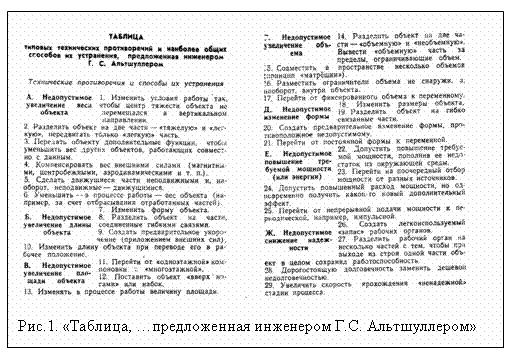
\includegraphics[width=.8\textwidth]{./10.jpg} \\
Рис. 1. Таблица типовых технических противоречий и наиболее общих способов их
устранения, предложенная инженером Г. С. Альтшуллером
\end{center}

Сравним Таблицу из книги Корнеева с «впервые составленной таблицей»,
опубликованной в 1964 году (см. часть 4 настоящего текста). Несмотря на
сплошную нумерацию приемов у Корнеева, в большинстве своем они легко
подставляются в Таблицу-1964, лишь изредка меняя свое положение.

Это и не удивительно. Ведь единственным качественным отличием «впервые
составленной таблицы» Альтшуллера 1964 года от «Таблицы, …предложенной
инженером Г.С. Альтшуллером» Корнееву в 1962 году, (как и от их средней сестры
1963 года), явилось появление верхней горизонтальной оси. В ней были
перечислены (основные) принципы устранения технических противоречий,
объединяющие приемы в семь групп.

Ни число групп приемов (сначала минимум шесть, затем семь), ни состав
ухудшаемых характеристик (десять), ни количество используемых приемов
(41-36-40) за три года принципиально не изменились. Зато дважды обновился
состав приемов, что подтверждало общую тенденцию постоянного расширения
Списка.

Для большей наглядности придадим «Корнеевской»
таблице\footnote{\url{https://metodolog.ru/00749/pic2.pdf}} соответствующую ее
статусу табличную форму, чтобы иметь возможность сравнить ее с наиболее
значительными последовательницами -- 1964-го и 1971-го годов.

Прежде всего, бросается в глаза то обстоятельство, что некоторые приемы
повторяют другие или почти полностью (8→19, 29→36, 38→39), или в очень
значительной степени (2→14, 17→21, 33→41, 8→31→34, 2→14→37, 9→20, 25→35).
Очевидность дублирования подсказывала, что часть приемов должна либо полностью
исчезнуть из дальнейших версий Таблицы, либо (в случае особой важности
разновидности) должна быть включенной в ее состав в качестве т. н. подприемов.

Вместе с тем встречаются приемы, комплексный характер которых не вызывает
сомнений. К ним можно отнести, прежде всего, № 31 «Разделить объект на части;
изготовлять каждую часть отдельно, затем производить сборку» и № 14 «Разделить
объект на две части -- 'объемную' и 'необъемную'. Вывести 'объемную' часть за
пределы, ограничивающие объем».

В общей сложности, в Таблице-1962 среди 41 приема «проявляются» в той или иной
степени более 20 типовых приемов, ставших после 1971 года «классическими«:
Генрих Саулович добавил в Таблицу 1964 года 4 новых «классических» приема, но
и удалил из нее 2 будущих «классических» приема: № 21 «Принцип проскока» и №
22 Принцип «обратить вред в пользу». На первый взгляд, такое обновление
кажется не совсем логичным. Но не следует забывать, что в 1964 году
непрерывное изменение Списка приемов свидетельствовало о творческом процессе
поиска. «Классического» постоянства от приемов еще не требовалось. По этой же
причине несколько позиций были в значительной степени переформулированы или
вовсе перераспределены между двумя вновь образовавшимися приемами (№№ 12,
30). 

\subsection*{Мечты сбываются}

Еще в 1961 в своей первой книге Альтшуллер упоминает о будущей Таблице только
как о желаемом инструменте изобретателя. А число пока еще весьма обще
сформулированных, отличающихся по своему действию Изобретательских Приемов
было еще относительно невелико -- ровным счетом 20 приемов, разделенных на
четыре группы:
\begin{quote}
  В качестве основы для таблицы могут послужить четыре группы приемов, с
  которыми мы уже познакомились. При пополнении таблицы можно не заботиться о
  строгости классификации. Достаточно, чтобы приемы располагались от простого
  к более сложным.
\end{quote}

И вот лишь через год после этого сообщения Альтшуллера редактор Корнеев
публикует в своей книжке Таблицу с 41 приемом, три четверти которых --
совершенно новые! То есть издает ее почти в том виде, в котором она появилась
«впервые» в 1964 году. Вот только приемы уже не разделены на группы (четыре
или более), а «привязаны» к десяти характеристикам, о которых в 1961 году еще
не было и речи. То есть, какая никакая, а классификация приемов (по целевому
назначению) стала очевидной.

Удалось ли Корнееву предвосхитить структуру «впервые составленной таблицы»
образца 1964 года, значительно расширив Список 1961 года и придав ему
табличную форму, сгруппировав по характеристикам? Или же это Альтшуллер сумел
за один лишь год доработать внезапно «созревшую» после разрыва с Шапиро идею?

А может быть, Корнеев, «первым из редакторов осознавший значение ТРИЗ для
человечества», просто решил таким необычным способом «подтолкнуть» Альтшуллера
к реализации найденного им, Корнеевым, раньше решения? Понимал, что дальнейшая
разработка Таблицы для него, Корнеева, дело непосильное? И теперь в своей
книге хотел подбодрить инженера Г. С. Альтшуллера? Мол, давай, парень, не
тушуйся, продвигай Таблицу! Нашу первую Таблицу.

Получить, ответить на эти вопросы мы уже вряд ли когда-нибудь сумеем. Но и не
задать их -- хотя бы самим себе -- мы тоже не вправе.

Само название Таблицы наводит внимательного читателя на размышления. Не
«Таблица Г. С. Альтшуллера», что было бы вполне естественным, если речь шла о
едином и неделимом авторе идеи. Но «Таблица …, предложенная инженером
Г. С. Альтшуллером», словно у молодого инженера появились доработки,
направленные на развитие какой-то уже существующей таблицы. Наверное, так
отреагировал бы сам Альтшуллер на возможные разработки своих учеников: «АРИЗ,
предложенный физиком Гориным…», «ЗРТС, предложенные изобретателем Злотиным» …
(Сравните -- «Гиперболоид, предложенный инженером Гариным…»)

Недоумение вызывает и другое обстоятельство, наводящее на мысль о том, что сам
инженер Г. С. Альтшуллер как будто еще ничего о предложенной им в 1962 году
Таблице не знал. В статье «Внимание: алгоритм изобретения!»
\cite{Altshuller1965}, он представил свои разработки последних лет. Прежде
всего, это -- список 35-ти «основных приемов устранения технических
противоречий», ставших позднее классическими, и новенькая симметричная Таблица
их применения с 16 характеристиками. В заключение этой фундаментальной работы
автор приводит список наиболее значительных изданий последних лет:

\paragraph{Литература по методике изобретательства}
\begin{itemize}
\item[] Г. С. Альтшуллер. Основы изобретательства. Центрально-черноземное
  книжное издательство, 1964.  
\item[] С. Г. Корнеев. Алгебра и гармония. Тамбовское книжное издательство,
  1964.
\item[] Д. Пойа. Как решать задачу. Учпедгиз, 1961.
\item[] A. И. Микулич. Некоторые вопросы машинной эвристики. Журнал
  «Зарубежная радиоэлектроника», 1964, №№ 10, 11.
\item[] Д. Биленкин. Путь через невозможно. Тамбовское книжное издательство,
  1964.
\item[] B. Н. Мухачев. Как рождаются изобретения. «Московский рабочий». 1964.
\end{itemize}
Как не трудно заметить, первая книга Корнеева \cite{Korneev1962} в этом списке
не фигурирует, как и сборник «Азбука рационализатора» \cite{Altshuller1963}, в
котором была опубликована следующая Таблица. Никогда не ссылался Альтшуллер на
эти издания и в своих более поздних книгах и публикациях. В «Алгоритме
Изобретения» он приводит выдержки из десятков книг и статей различных авторов.
Но собственные работы 1962-63 годов не упоминаются и здесь ни словом.

Молчанием автор обошел их и в книгах 1968, 1973, 1979 годов. Возможно ли,
чтобы Альтшуллер забыл о собственном приоритете 1962 года? Или хотел забыть о
книгах, в которых действительно впервые были опубликованы «его» Таблицы? А
может быть, просто старался больше не вспоминать о «Таблице, предложенной
инженером Альтшуллером«?

Возможно, Альтшуллер и шутил, говоря о том, что идею и термин «физического
противоречия» подарил ему некто Перельштейн \cite{Filkovsky2006}. О том, кто
подарил ему идею Таблицы, Альтшуллер даже и не шутил.
\begin{quote}
  Все слушатели должны накрепко усвоить, … что число типов технических
  противоречий сравнительно невелико, и что существуют поэтому типовые приемы
  их устранения. В книге «Основы изобретательства» есть большая
  иллюстрированная таблица таких противоречий и способов их устранения.
  \cite{Korneev1964}
\end{quote}
Этот рекламный анонс появился во второй книге Корнеева «Алгебра и гармония» в
начале 1964 года. О том, что в его книге «Тайны творчества» Таблица была еще
больше, автор скромно умолчал. Возможно, именно он убедил Альтшуллера в том,
что «число типов технических противоречий сравнительно невелико».

Готовя к выпуску новую книгу Альтшуллера, редактор заранее предвкушал ее успех
и стремился всячески его подкрепить. Но Станислав Георгиевич Корнеев вскоре
трагически погиб, спасая из затопленного редакционного подвала тиражи книг. И
издание «Основ изобретательства» \cite{Altshuller1964} было перенесено в
Воронежское издательство на конец 1964 года.

\subsection*{Редактор или исследователь методики изобретательства?}

В «Алгебре и гармонии» редактор Корнеев не просто уделил изобретательским
приемам большое внимание. Его вклад в развитие этой темы сегодня можно было бы
назвать серьезной авторской разработкой. Ведь, кроме всего прочего, он
предложил и свою классификацию приемов:
\begin{quote}
  Типовые приемы можно разделить на два вида. Прежде всего -- основные
  принципы изменения технических систем (принцип дробления, принцип
  динамичности и т. д.). Такие принципы накапливаются по мере развития
  техники. … Принципы оказались универсальными, поэтому с их помощью и по сей
  день можно решать различные изобретательские задачи. И хотя каждый такой
  принцип сам по себе уже известен, каждое конкретное применение считается
  новым изобретением, если при этом удается устранить техническое
  противоречие. … Другая группа приемов -- это методы, основанные на
  использовании новых материалов, новых видов энергии и т. д.
\end{quote}
«Основные принципы» хорошо смотрелись и уверенно звучали. То, что в короткой
формулировке была заложена тавтология (принцип [лат. principium -- основа,
  начало] -- основное положение), Корнеева, а позднее и Альтшуллера не
смущало.

Корнеев смотрел далеко вперед и предвидел значительные преобразования в
Таблице. Прежде всего, за счет новых приемов, таких как «использование
пневмоконструкций, оптического моделирования и т. д.». То есть тех самых, на
которые ни в Таблице «предложенной инженером Альтшуллером» в книге Корнеева в
1962 году, ни в Таблице 1964 года, опубликованной самим Альтшуллером, нет ни
малейшего намека. Своими рассуждениями Корнеев словно бы задавал тон «инженеру
Альтшуллеру», указывая на направление необходимых в будущем расширений.

Корнеев пророчески заглядывал еще дальше, предрекая «выпадение» из Таблицы
«конструкторских приемов, которые в силу своей новизны пока являются
изобретательскими». Уже в 1964-м году Корнеев предвидел и дальнейший рост
Таблицы, и ее становление, и даже «отмирание» отдельных ее частей (как тут не
вспомнить о ЗРТС?):
\begin{quote}
  Пройдет время, и часть таких приемов будет отнесена к «вечным» принципам, а
  часть станет общеизвестными способами решения технических задач, а не будет
  считаться изобретательством.
\end{quote}
\clearpage

\begin{flushright}
  «Мысли об истории делают меня пессимистом …\\
  Но мысли о предыстории делают меня оптимистом»\\
  Ян Сматс
\end{flushright}
\section*{7. АРИЗ(К)-61}

На «Таблице…, предложенной инженером Альтшуллером» можно было бы завершить
ретроспективное изучении истории возникновения «самого главного инструмента»
ТРИЗ. Признать альтшуллеровский вариант корнеевской Таблицы первым упоминанием
о ней в публикациях, связанных с ТРИЗ. И закрыть дело.

Или пусть это будет корнеевский вариант альтшуллеровской Таблицы? Назвать ее
для простоты Таблицей Корнеева-Альтшуллера и присвоить ей Минус Второй номер.
А кто автор, -- ну, кого это сегодня может волновать? Главное -- теперь мы
точно знаем, когда она возникла.

Стоп! А знаем ли мы это точно? Таблицу Корнеева-Альтшуллера мы датировали 1962
годом, основываясь на времени издания брошюры Корнеева «Тайны творчества»
\cite{Korneev1962}. Чтобы, так сказать, не усложнять Историю ТРИЗ еще больше.
Она уже написана и утверждена. И переделать ее трудно. Разве что только
переосмыслить.

Ведь историю АРИЗ Генрих Саулович писал в 1986 году \cite{Altshuller1986a}.  И
хотя память у него была отменная, да только отношение к событиям давно
прошедших дней вполне могло измениться. Тем более, что попытки
документирования истории ТРИЗ вызывали сложности не только у него. Задача эта
не из легких, особенно 25 лет спустя. Но и увлекательная, -- открываются
дополнительные просторы для фантазии.

Как меняются порой взгляды на события давно минувших дней, объяснять не надо.
Достаточно поинтересоваться мнением ближайших соратников:
\begin{quote}
  Не нужно забывать, что людям свойственно развиваться и менять свои мнения.
  Это значит, что Б. Злотин сегодня вполне может быть совершенно не согласен с
  мнением, высказанным в статье Б. Злотина написанной 20 лет назад.
  \cite{ZlotinZusmanNN}
\end{quote}
Корнеев словно предвидел возможные проблемы и «предусмотрел» для нас
возможность заглянуть в прошлое, чтобы не ошибаться. В своей брошюре 1962 года
\cite{Korneev1962} он привел описание трех стадий поиска и устранения
технического противоречия -- аналитической, оперативной и синтетической. И
предложил:
\begin{quote}
  Проследим на конкретном примере, как ведется систематическое решение задачи.
  (\textbf{Этот пример разбирался на семинаре по методике, проводившемся в
    Тамбове в 1961 году}. Выделено нами -- Л.Ш.).
\end{quote}
Решение в приведенном примере проводилось на оперативной стадии уже знакомым
нам по АРИЗ-65 способом:
\begin{quote}
  По таблице это способы с № 36 по № 41.

  № 36 -- изменить скорость процесса. Опытный изобретатель догадается, что… и
  т.д.
\end{quote}
Получается, что Таблица с 41 приемом, десятью характеристиками и семью
группами приемов (пока еще не явно выраженными принципами) применялась на
семинарах по ТРИЗ уже в 1961 году?!

Но первоисточники мы изучали добросовестно и твердо усвоили, что в 1961 году
приемов было ровно двадцать, разделены они были на четыре группы, и ни о какой
привязке их к характеристикам даже речи не было! Не говоря уже о какой-то
Таблице. Так что, товарищ Корнеев, сами придумали, сами и внедряйте!

Именно так Станислав Георгиевич и поступил. В своей брошюре он изложил новый,
расширенный вариант АРИЗ, в котором Таблице было отведено важное -- если не
сказать, центральное -- место. Назовем этот вариант \textbf{АРИЗ
  Корнеева-Альтшуллера или АРИЗ(К)-61}, ведь в официальных материалах по ТРИЗ
он не фигурирует.

Обратимся к описанию предложенного Корнеевым алгоритма:
\begin{quote}
  \textbf{Теория изобретательства} (Выделено нами -- Л.Ш.) использует давно
  применяющийся в математике метод разложения трудной операции на сумму
  относительно простых действий. Теория учит, как шаг за шагом вести поиски
  технического противоречия (оно не всегда лежит на виду) и как его устранить.
  Вот эти шаги: …
\end{quote}
В предлагаемой сравнительной таблице \cite{Shub2006} \textbf{АРИЗ(К)-61}
помещен между \textbf{АРИЗ-61} и \textbf{АРИЗ-64}. Хотя, возможно, располагать
его следовало бы сразу после \textbf{АРИЗ-59}. К сожалению, о точном времени
создания этой версии Корнеев ничего не говорит. В качестве первого
официального «табличного» алгоритма здесь приводится и \textbf{АРИЗ-65}.

Наиболее важным для тематики предлагаемой работы новшеством явилась введенная
в \textbf{АРИЗ(К)-61} на первом шаге оперативной стадии 
\begin{quote}\bf
  проверка возможности устранения технического противоречия по «Таблице
  типовых технических противоречий и наиболее общих способов их устранения,
  предложенной инженером Г.С. Альтшуллером.
\end{quote}

У Генриха Сауловича (и в Истории АРИЗ \cite{Altshuller1986a}) Таблица
появилась лишь в АРИЗ-65.  Правда, уже в АРИЗ-64 четыре шага (группы приемов)
оперативной стадии были предварительно попарно сведены в первый и второй шаги,
что выглядело вполне логично перед окончательным свертыванием всего Списка.
Если бы только Корнеев не «свернул» эти четыре шага в один -- Таблицу -- уже в
1961 году!

\textbf{АРИЗ(К)-61} содержит и другие интересные новшества, отличающие его как
от предыдущей (АРИЗ-61), так и от последующей (АРИЗ-64) версий алгоритма:
\begin{itemize}
\item \textbf{В АРИЗ(К)-61} из аналитической стадии выведена «постановка
  задачи» на первом шаге, а стадия начинается сразу с определения идеального
  желаемого результата. В значительной степени это определение стало предтечей
  будущего «шага назад от ИКР», снижая планку психологического барьера перед
  выбором цели.
\item Сделана попытка сконцентрировать внимание изобретателя на физической и
  химической природе возникновения технического противоречия:

  \textbf{Третий шаг аналитической стадии:}

  Определить, почему мешает (ответить на вопрос: В чем непосредственная --
  \textbf{физическая или химическая} -- причина этой «помехи»?);
\item Впервые поставлен акцент на понятии технического противоречия:

  \textbf{Четвертый шаг аналитической стадии:}

  Определить, при каких условиях не мешало бы (ответить на вопрос: При каких
  условиях исчезнет «помеха», \textbf{вызывающая данное техническое
    противоречие}?).

  Заметим, что это была последняя попытка направить логику АРИЗ на устранение
  собственно \textbf{причины} технического противоречия. Начиная с АРИЗ-64
  вопрос «В чем непосредственная причина «помехи»?» хотя и задавался, но под
  идеальным результатом уже понимался ответ на вопрос: «При каких условиях
  \textbf{исчезнет «помеха»}?«
\item Наконец, в \textbf{АРИЗ(К)-61} «промелькнул» и предложенный еще в 1956
  году как «Последний этап творческой работы -- оценка сделанного изобретения»
  четвертый шаг синтетической стадии:
  \begin{quote}
    Оценить полученную идею изобретения.
  \end{quote}
  
Официально реализован и закреплен в тексте алгоритма этот шаг был лишь через
10 лет в АРИЗ-71 \url{Altshuller1971}.
\end{itemize}

Отдавая дань самоотдаче, с которой С.Г. Корнеев поддерживал развитие методики,
и той корректности, с которой он относился к приоритетам, следует отметить,
что авторство Альтшуллера он отметил только за опубликованным в книге
вариантом Таблицы.

Что касается последовательности шагов в «процессе поиска технического
противоречия», то есть в \textbf{АРИЗ(К)-61}, то здесь он не назвал имен
авторов, а использовал обобщающее понятие «Теория изобретательства».

\subsection*{Открытые вопросы}

Нетрудно заметить, что предлагаемый у Корнеева список шагов
(\textbf{АРИЗ(К)-61}) нарушает эволюционную последовательность версий АРИЗ,
«перепрыгивая» через следующий за ним лишь через три года АРИЗ-64.

Что же помешало Альтшуллеру включить Таблицу в состав АРИЗ-64? Вернее, что
заставило его удалить уже отработанную на нескольких семинарах Таблицу из
\textbf{АРИЗ(К)-61}? Что не позволяло ему упоминать об этой разработке в
книгах 1968-71-79 годов? Что удерживало от упоминаний истинного времени ее
появления на свет, как и о двух книг, в которых рождение и развитие Таблицы
было документально зафиксировано? И почему это «что-то» уже не помешало
включить лишь непринципиально измененную за четыре года Таблицу в состав
АРИЗ-65?

Ответы на эти вопросы вряд ли окажутся простыми, даже если принять, что
Альтшуллер всегда корректно ссылался на собственные разработки и не слишком
охотно упоминал опережающие разработки других авторов.

Книга «Основы изобретательства» \cite{Altshuller1964} вышла в 1964 году в
Воронежском издательстве и была посвящена светлой памяти Г.С. Корнеева. Памяти
редактора, который в 1961 году «осмелился» пойти вперед, обгоняя Альтшуллера,
не только дав ему идею Таблицы и многочисленные новые приемы для ее
заполнения, но и найдя для этой разработки соответствующее место в АРИЗ.
Место, которое сам Альтшуллер затем «подыскивал» еще несколько лет.

Имеющаяся у нас информация достаточно скупа и позволяет лишь предположить
равноправность творческого союза Альтшуллера с еще одним разработчиком и
соавтором АРИЗ в 1961--1964 годах. Признавать подобные союзы Генрих Саулович
не очень любил. И многих учеников своих от мыслей об этом отучил раз и
навсегда.

Поможет ли это предположение объяснить «прыжок» от \textbf{20} приемов в
\textbf{АРИЗ-61} к \textbf{41} приему (три четверти из которых -- новые) в
\textbf{АРИЗ(К)-61}? Как и их сведение в Таблицу! Или отказ от простой и до
сих пор логичной классификации приемов по группам. Или тот факт, что отдельные
шаги алгоритма, включенные самим Альтшуллером в состав АРИЗ лишь в 1965--1971
годах, существовали и были опробованы уже в 1961 году.

Рассуждения Корнеева свежи и оригинальны, порой они опережают соответствующие
разработки Альтшуллера. Корнеев говорил о новых приемах, таких как
«использование пневмоконструкций, использование оптического моделирования и
т. д.», как бы обращая внимание Альтшуллера на перспективные направления
оптимизации состава Списка.

Одновременно Корнеев сместил акцент с расширения Списка за счет новых приемов
на их организацию в Таблицу и классификацию по изменяющимся характеристикам,
на которые эти приемы «реагировали».

Белых пятен в истории ТРИЗ много. Вопрос о том, кто и в какой степени
участвовал в создании «Таблицы …, предложенной инженером Альтшуллером»,
возможно, так и останется открытым. Но сколько интересного, оказывается, можно
найти и во «вторичных» первоисточниках ТРИЗ!

А пока что достаточно обоснованно можно считать, что Таблица интенсивно
«обкатывалась» на семинаре по ТРИЗ в Тамбове уже в 1961 году.
\clearpage

\begin{thebibliography}{xxx}
\bibitem{Altshuller1956} Г.С. Альтшуллер, Р.Б. Шапиро. О психологии
  изобретательского творчества.  Вопросы психологии, 1956, № 6, стр. 37-49.
  \url{http://www.altshuller.ru/triz0.asp}
\bibitem{Altshuller1959} Г.С. Альтшуллер, Р.Б. Шапиро. Изгнание шестикрылого
  серафима. Изобретатель и рационализатор, 1959. № 10.
  \url{http://www.altshuller.ru/triz12.asp}
\bibitem{Altshuller1961} Г.С. Альтшуллер. Как научиться изобретать. Тамбов:
  Книжное издательство, 1961.  \url{http://www.altshuller.ru/triz/triz49.asp} 
\bibitem{Altshuller1963} Г.С. Альтшуллер. Как работать над изобретением.
  \emph{Азбука рационализатора}, Сост. Б. Зубков, Ю. Медведев, С. Муслин. --
  Тамбов: Кн. изд-во, 1963.
\bibitem{Altshuller1964} Г.С. Альтшуллер. Основы изобретательства. – Воронеж:
  Центрально-черноземное книжное издательство, Воронеж, 1964.
  \url{http://www.altshuller.ru/triz/ariz64.asp}
\bibitem{Altshuller1965} Г.С. Альтшуллер. Внимание: алгоритм изобретения!,
  Технико-экономические знания: приложение к «Экономической газете»,
  01.09.1965, -- Вып. 27(41).
\bibitem{Altshuller1971} Г.С. Альтшуллер.  Алгоритм решения изобретательских
  задач АРИЗ-71. – Баку: ОИИТ при ЦК ЛКСМ Азербайджана и Азербайджанском РС
  ВОИР, 1971. \url{http://www.altshuller.ru/triz/ariz71.asp}
\bibitem{Altshuller1974} Г.С. Альтшуллер. Планы занятий на первом курсе
  АзОИИТ.  1973--74. \url{http://www.altshuller.ru/engineering6.asp}.
\bibitem{Altshuller1975} Г.С. Альтшуллер, Г.Л. Фильковский. Современное
  состояние Теории Решения Изобретательских Задач. 1975.
  \url{http://www.altshuller.ru/triz2.asp}.
\bibitem{Altshuller1979} Г.С. Альтшуллер. Творчество как точная наука: Теория
  решения изобретательских задач. М.: Сов. радио, 1979.
\bibitem{Altshuller1985} Г.С. Альтшуллер. Письмо 19.  31.01.1985.
  \url{https://www.altshuller.ru/corr/correspondence1.asp#19}
\bibitem{Altshuller1986} Г.С. Альтшуллер. Жизнь Человека 1-Ч-502, рассказанная
  Игорю Верткину, 1985-1986.
  \url{https://www.altshuller.ru/interview/interview5.asp}.
\bibitem{Altshuller1986a} Г.С. Альтшуллер.  История Развития АРИЗ (конспект).
  1986.  \url{http://www.altshuller.ru/triz/ariz-about1.asp}
\bibitem{Altshuller1994} Г.С. Альтшуллер, И.М. Верткин. Как стать гением:
  Жизненная стратегия творческой личности. -- Минск, Беларусь, 1994.
  \url{http://www.altshuller.ru/trtl/heretic2.asp}
\bibitem{Altshuller1996} Г.С. Альтшуллер. Ответы на вопросы Джеймса Ковалика.
  16.06.1996.  \url{https://www.altshuller.ru/interview/interview4.asp}.
\bibitem{Amnuel964} П. Амнуэль. Старик Жюль Верн и космическая эра. Молодежь
  Азербайджана, Баку 1964.  \url{http://www.fandom.ru/}.
\bibitem{Bachmatov1961} Р. Бахтамов. Изгнание шестикрылого серафима, М.:
  Детгиз, 1961.  
\bibitem{Blaesing2001} Jürgen P. Bläsing, Walter Brunner. TRIZ. Von der
  Theorie zur Praxis. Für TRIZ Moderatoren und TRIZ Teams. Mit der
  Konflikt-Matrix in DIN A2, Ausgabe 2001.
\bibitem{Dworschak2005} Manfred Dworschak. Zwergenarmeen im Kopf. Der
  Spiegel, 30/2005, S. 114.
\bibitem{Filkovsky2006} Г. Фильковский (2006). «Горин -- автор идеи
  физического противоречия ???!!!».
  \url{http://www3.sympatico.ca/karasik/GF_re_gorin_claim.html}
\bibitem{Gimpel2000} Bernd Gimpel, Rolf Herb, Thilo Herb. Ideen finden,
  Produkte entwickeln mit TRIZ. Hanser Verlag, 2000.
\bibitem{Herb2000} Rolf Herb, Thilo Herb, Veit Kohnhauser. TRIZ, der
  systematische Weg zur Innovation. Verlag Moderne Industrie, 2000.deen finden,
  Produkte entwickeln mit TRIZ. Hanser Verlag, 2000.
\bibitem{Jacobson1934}  П.М. Якобсон. Процесс творческой работы изобретателя.
  1934. 
\bibitem{Korneev1962} С.Г. Корнеев, Тайны творчества, Тамбов, 1962,
  Библиотечка новатора.  \url{https://www.metodolog.ru/00696/00696.html} 
\bibitem{Korneev1964} С.Г. Корнеев, Алгебра и гармония, Тамбов, 1964.
  (Библиотечка новатора; Вып. 2),
  \url{http://www.metodolog.ru/00630/00630.html}
\bibitem{Korolyev1998} В.А. Королёв. Современные тенденции развития АРИЗ.
  25.01.1998. \url{http://www.triz.org.ua/data/w55.html}
\bibitem{Kudryavtsev} А.В. Кудрявцев. Как выбирать приемы для решения.
  Учебник по ТРИЗ. гл. 8.  \url{http://metodolog.ru/00088/00088.html}
\bibitem{Leon2005} Noel Leon, Jose Jesus Martinez, Carlos Castillo.
  Methodology for the Evaluation of the Innovation Level of Products and
  Processes. TRIZ Journal 10/2005.
\bibitem{Livotov2004} P. Livotov. TRIZ im Innovationsprozess. Konstruktion \&
  Engineering, 03/2004.
\bibitem{Livotov2005} P. Livotov, D. Murnikov. Innovation als Prozess. 
  4. TRIZ-Kongress, Frankfurt, 29. Juni 2005. 
\bibitem{Mann2005a} Darrell Mann, Conall Ó Catháin.  Using TRIZ in
  Architecture: First Steps. TRIZ Journal 11/2005.
\bibitem{Mann2005b} Darrell Mann, Chris Bradshaw. Design for Wow 2 – Music.
  TRIZ Journal 10/2005.
\bibitem{MATRIZ2003} МА ТРИЗ. Проект Положения о многоступенчатой аттестации
  пользователей и сертификации специалистов Международной Ассоциации ТРИЗ.
  Принято на заседании Президиума МА ТРИЗ, 26 июня 2003 г.
  \url{https://triz-summit.ru/triz/history/300029/matriz-2003/300314/300315/}.
\bibitem{Murashkovsky2003} Письмо от Ю.С. Мурашковского. 03.10.2003.
  \url{https://subscribe.ru/archive/science.natural.triz/200310/03201643.html}.
\bibitem{Murashkovsky2006} Ю.С. Мурашковский, Детская болезнь
  «ниспровержизма». 22.03.2006, не опубликован.
  \url{https://subscribe.ru/archive/science.natural.triz/200310/03201643.html}.
\bibitem{OrlovNN} В. Орлов, Трактат о вдохновении, рождающем великие
  изобретения.  \url{https://www.metodolog.ru/00193/00193.html}
\bibitem{Salamatov1992} Ю.П.Саламатов. Современное состояние и проблемы
  развития ИМ-ТРИЗ-технологии. Минск, 19-21 мая 1992 г.
  \url{http://www.triz-guide.com/publicat/articles/article7.html}
\bibitem{Shub2004} Л. Шуб. Особенности распространения и видоизменения ТРИЗ в
  центральной Европе (1998--2004).
  \url{http://metodolog.ru/00452/00452.html}.
\bibitem{Shub2006} Л. Шуб. Сравнительная таблица изменений и перемещений в
  ранних версиях АРИЗ. \url{https://metodolog.ru/00908/00908.pdf}
\bibitem{Sietmann2001} Richard Sietmann. Erfinden nach Plan. c't -- Magazin
  fur Computertechnik 23/01, Seite 96.
\bibitem{Stuart2005} Jack Stuart. Transactional TRIZ, Theory, Application, and
  Execution, Part II: The Contradiction Matrix. TRIZ Journal 10/2005.
\bibitem{Teufelsdorfer1998} A. Teufelsdorfer, A.  Conrad. Kreatives Entwickeln
  und innovatives Problemlösen mit TRIZ/TIPS, Publicis MCD Verlag, Erlangen
  und München 1998.
\bibitem{Terninko1998} John Terninko, Alla Zusman, Boris Zlotin. TRIZ -- Der
  Weg zum konkurrenzlosen Erfolgsprodukt. Verlag Moderne Industrie, 1998.
\bibitem{ZlotinZusmanNN} Б. Злотин, А. Зусман, «О попытке документирования
  истории ТРИЗ»,
  \url{http://www.trizscientific.com/TRIZ_sci/history/history_main_r.htm}
\end{thebibliography}


\end{document}

%=============================================================
Часть 8

Магический квадрат

Потребовалось исследовать не 2 тысячи,
а 200 тысяч наиболее сильных изобретений

Альтшуллер Г.С. «Душа обязана… учиться»,
Литературная газета, 1980, 4 июня (№23)

После достаточно продолжительного экскурса в прошлое «табличной» ТРИЗ пришло время подводить итоги историческому обзору и рассмотреть заключительный этап в развитии ее, если не самого важного, то наиболее часто употребляемого элемента.

В 1961 году впервые была предпринята попытка отказаться от классификации приемов по группам, чтобы «привязать» их к ухудшающимся параметрам технической системы. Долгое время ухудшение одного из параметров технической системы трактовалось как проявление собственно технического противоречия, что несколько затормозило развитие табличного механизма управления выбором подходящего приема. В значительной степени способствовало этому представление С.Г. Корнеева о том, что «число типов технических противоречий сравнительно невелико, и что существуют поэтому типовые приемы их устранения». [С. Корнеев, Алгебра и гармония, Тамбов, 1964. (Библиотечка новатора; Вып. 2), http://www.metodolog.ru/00630/00630.html].

Сегодня одностороннее негативное изменение состояния технической системы представляется очевидной подменой собственно технического противоречия (в его классической формулировке). Но 40 лет назад это допущение явилось, несомненно, значительным прогрессом на пути к универсальной Таблице. Тем не менее, очередная Таблица 1963 года, содержавшая только 36 приемов после 41, опубликованных в «Корнеевской» версии описания АРИЗ в -61 году, не несла в себе принципиальных изменений, отразив лишь безостановочный процесс поиска новых приемов и оптимизации Списка типовых приемов.

Следующая за нею Таблица-1964 (40 приемов) была, по сути, первой и последней попыткой гибридизации двух подходов -- прежней классификации приемов по группам (по горизонтальной оси) и их привязки к ухудшающимся параметрам технической системы (по вертикальной оси). Считавшаяся самим Альтшуллером «впервые составленной», она может рассматриваться нами, пожалуй, лишь как промежуточный эксперимент на пути к созданию действительно мощного, поражающего воображение инструмента -- симметричной Таблицы.

В сентябре 1965 года в статье «Внимание: алгоритм изобретения!» [Альтшуллер Г.С, «Внимание: алгоритм изобретения!», Технико-экономические знания: приложение к «Экономической газете», 01.09.1965, -- Вып. 27(41), www.altshuller.ru/triz/triz022.asp] в составе нового АРИЗ-65 была опубликована «Таблица использования приемов устранения технических противоречий», положившая начало новому семейству тризных инструментов -- симметричных Таблиц.

Рис. 1, Симметричная Таблица в АРИЗ-65

Эта Таблица включала 16 технических характеристик, то есть тех «типовых» параметров технических систем, недопустимые ухудшения которые в прежних версиях воспринимались как технические противоречия.

Как и предыдущие версии, она предназначалась для систематизированного выбора и применение приемов устранения технических противоречий. А использованные в ней 35 приемов, вошедшие (несмотря на более поздние подмены) в историю ТРИЗ как «основные», стали по сути «классическими».

Само по себе расширение группы характеристик шестью новыми представительницами за четыре года было значительным развитием нового инструмента. Но этот количественный скачок в сочетании с новой, симметричной архитектурой привел к значительно более важным, качественным изменениям в структуре Таблицы и теоретических возможностях ее использования.

Ухудшающиеся («недопустимо изменяющиеся, если решать задачу известными способами«) характеристики или технические параметры располагались по горизонтальной оси. А вертикальная ось была на этот раз представлена теми характеристикам объекта, которые требовалось улучшить по условиям задачи. А вернее, теми же характеристикам, поскольку состав обеих осей новой Таблицы был идентичен. Техническим противоречиям (или «конфликтным парам«) уже не отводилась, как в 1961-1964 гг., роль базовых параметров. Их формирование производилось путем скрещивания уже упомянутых основных (типовых) технических характеристик системы.

Уже в Таблице-64 приемы приобрели характер векторов, направленных на ИКР и имеющих в основании недопустимо ухудшающиеся характеристики. (Осторожно! Таблица технических противоречий. Часть 4, Рис. 1).

В новой Таблице поиск решения велся уже «перекрестным огнем». Это создавало еще большую убедительность возможности достижения ИКР, скрытого за противоречием (помехой), наикратчайшим путем. Нужно было лишь правильно определить конфликтную пару, чтобы, пользуясь указанными в клетке пересечения двух векторов направлениями действия (номерами приемов), гарантирующими наибольший успех, сбросить камень противоречия.

Во всех трех предыдущих версиях Таблицы предлагались только 10 «типовых технических противоречий», снабженные четырьмя десятками единичных рекомендаций по применению приемов.

Сразу 240 технических противоречий (конфликтных пар), представленные в новом варианте, однозначно свидетельствовали о революционных изменениях в философии методики изобретательства. Не менее грандиозно, должно быть, выглядели в 1965 году и 578 отдельных рекомендаций по использованию 35-ти Основных приемов, расставленные в клетки Таблицы (пока еще очень неравномерно -- от пустых клеток до четырех приемов в одной клетке).

Осуществился одновременно количественный и качественный рывок, отразивший и перемену в представлениях Г.С. Альтшуллера, теперь уже единоличного автора Таблицы, о том, насколько же «невелико» может быть число типовых технических противоречий в действительности. Изобретательскому братству была представлена счастливая находка, своего рода методическая инновация. Она позволяла быстро и планомерно, а фактически произвольно генерировать любое число «типовых технических противоречий».

Возникшую при этом (впрочем, далеко не первую в истории ТРИЗ) опасность подмены статистической реальности желаемым идеалом, выдаваемым за результат научного поиска, автор попросту проигнорировал. Или не заметил. Сами технические характеристики, пока еще немногочисленные, можно было достаточно убедительно представить как результат статистического анализа имеющихся наработок тысяч реальных изобретательских задач. Но их механистическое скрещивание друг с другом, ведущее к автоматическому образованию множества новых конфликтных пар, было рискованной натяжкой.

И все же переворот свершился. Настало время Новой Изобретательской Политики:

- Еще в 1964 году «число типов технических противоречий сравнительно невелико», и поэтому «существуют типовые приемы их устранения». Типов технических противоречий насчитывалось лишь десять. Приемов же было выделено, по крайней мере, в четыре раза больше.

- В 1965 году число типовых технических противоречий одним махом перескочило за две сотни, а Список содержал по-прежнему неполные четыре десятка приемов.

- Еще в 1964 году было справедливо: «Когда техническое противоречие выявлено, изобретатель должен, не полагаясь на память, взять лист с таблицей приемов и последовательно проверить пригодность каждого приема». (Альтшуллер Г. Как научиться изобретать. -- Тамбов: Тамбовское книжное издательство, 1961)

- С 1965 года памятью изобретателя стала Таблица, а всякая попытка «последовательно проверить пригодность каждого приема» преследовалась со всей строгостью изобретательского закона.

- Еще в 1964 году «при пополнении таблицы можно не заботиться о строгости классификации. Достаточно, чтобы приемы располагались от простого к более сложным».

- В 1965 году «строгость классификации» определяла, фактически, успех всего предприятия. Любое даже самое легкое подозрение в недостаточной объективности при выделении приемов или необоснованности заполнения клеток рекомендациями было бы губительным.

- Еще в 1964 году следовало «Проверить без спешки, не отдавая заранее предпочтения тому или иному приему, не пропуская приемы, кажущиеся «заведомо непригодными». Очень часто лучшее решение дают именно эти заведомо непригодные приемы».

- В 1965 году путь к «заведомо непригодным» приемам оказался отрезанным границами той клетки Таблицы, в которой решателю отводилось не более четырех попыток, а предлагаемые приемы декларировались как самые лучшие.

И за всеми этими преобразованиями стояло магическое слово -- СТАТИСТИКА!

В начале 60-х Альтшуллер загорелся идеей Эвротрона. Возможно, это произошло после знакомства с современными механическими арифмометрами. Как и большинство гениев-автодидактов, недостаток регулярного образования он компенсировал мощным ассоциативным мышлением и тем, что сегодня принято называть «использованием информационных ресурсов».

Статистике в ТРИЗ была предназначена роль мессии, указующего перста, Спасителя, перенимающего на себя всю ответственность на полученные результаты и выводы. Но, прежде всего, с ее помощью можно было вывести Приемы из создавшегося тупика многообразия, в котором терялась вся их привлекательность.

Априори декларировалось, что для каждой из представленных характеристик непременно должно существовать некоторое множество технических систем (или их производных во времени и пространстве), состоящее из 15 групп. В каждой из этих групп улучшение основной характеристики приводит к однозначному ухудшению одной из оставшихся характеристик (основных параметров технической системы). А, однажды спрогнозировав такие технические системы, следовало их найти и «приручить».

Вспомним:

«Шапиро очень быстро оценил нашу перспективу…: «Маркс вывел законы развития общества, Дарвин вывел законы развития живых организмов, а мы выведем теорию, которая даст миру законы развития технических систем«». [Г.С. Альтшуллер, Жизнь Человека 1-Ч-502, 1985-1986, www.altshuller.ru].

Если до законов развития технических систем пока еще было далеко, то своеобразное универсальное правило прогнозирования неограниченного количества таких систем (вернее, их моделей в виде конфликтных пар) уже сформировалось. Следовало лишь открывать или создавать новые характеристики, и число новых конфликтных пар возрастало, как по мановению волшебной палочки, на многие десятки и даже сотни. И все их требовалось не только найти, но и «заранее вылечить», подобрав соответствующие приемы! Задача, вполне подходящая для Достойной Цели.

Возможно, именно трудности корректного выявления примеров и их приписки к соответствующей конфликтной паре и явились причиной того, что более половины клеток были снабжены только одним или двумя (соответственно 58 и 60 клеток) рекомендуемыми приемами.

Сколько именно конкретных примеров стояло за каждым из этих указаний, нигде не упоминалось. Все же следует отметить настойчивость автора: важной особенностью этой Таблицы было малое число пустых клеток. Только для семи конфликтных пар не были предусмотрены рекомендации приемов для устранения противоречия.

Советское -- значит короткое!

Можно строить различные предположения о том, что дало Альтшуллеру основание надеяться на создание функциональной и жизнеспособной Таблицы. Основная идея ее создания была столь же проста, сколь гениальна, и базировалась на характерной особенности составления патентной документации в Советском Союзе послевоенных десятилетий.

Структура описания изобретения к советскому авторскому свидетельству образца 50-х -- 60-х годов -- с формулой изобретения на первой странице, -- позволяла достаточно быстро ознакомиться с основной идеей изобретения. Нередко все описание умещалось на страничку, реже -- растягивалось на две.

Данные, определяющие методическую ценность (уровень) изобретения и применимость используемого в нем решения для статистической обработки, а порой и техническое противоречие в свободной формулировке зачастую присутствовали уже в самой «формуле изобретения» (на рисунке обведена красной линией).

Собственно техническое противоречие, преодоленное в изобретении, в традиционном для «классической» ТРИЗ виде, конечно, не формулировалось и оставалось для неосведомленного читателя неочевидным. Но от поисковика, вооруженного основами ТРИЗ, оно укрыться не могло, впрочем, как и способ (прием) его преодоления, -- такова была основная предпосылка для создания Таблицы.

Не укроются эти сведения от читателей и в предлагаемом примере более позднего периода (Рис. 2):

«СПОСОБ ВОЗДЕЙСТВИЯ НА СВЕРХЗВУКОВОЙ ПОТОК, обтекающий твердые тела, путём подачи струи газа из головной части тела навстречу набегающему потоку, отличающийся тем, что, с целью снижения лобового сопротивления тела, в струю газа дополнительно вводят частицы твердых материалов». (А.с. № 906203)

Рис. 2, Советское авторское свидетельство

По сравнению с «вычиткой» современного западного патента, затраты времени на поиск требуемой информации в советском авторском свидетельстве были незначительными. При определенных навыках, концентрации внимания и некотором везении (а также при наличии изначальных установок) предварительная обработка одного авторского свидетельства, облегчающая грубый отсев документов, занимала считанные минуты.

Именно это (скажем прямо, счастливое -- по крайней мере, до середины 60-х) обстоятельство и послужило идеологической основой создания Списка, а затем и отправной точкой в формировании информационного (статистического) фонда для Таблицы. Наглядность и кажущаяся простота выделения из патентного описанния не только технического противоречия, но и разрешающего его приема, представляются многим последователям Альтшуллера очевидными по сей день.

Эта гениальная идея не раз ложилась в основу принципов создания информационного фонда и для других разработок. В значительной степени она способствовала и созданию ауры исключительности, абсолютной истинности и непреложности, окружающей Таблицу и связанные с нею цифры до сих пор.

Непонимание того, с какими по объему и сложности документами приходилось иметь дело Альтшуллеру и его соратникам на заре создания ТРИЗ, а вернее перенос собственных представлений о современном патенте на приводимые в первоисточниках по ТРИЗ цифры («выросшие» в последние годы до миллионов) и приводит западного инженера в священный трепет. Одновременно это служит прочной психической защитой от любых попыток ревизии, как самой Таблицы, так и Списка.

Правда, редко кому приходит в голову задаться вопросом о том, какая же именно часть описаний попадает в «отходы» лишь по той причине, что скрытые в них технические противоречия, используемые решения или приемы содержались в неявном, неудобном для статистической обработки виде или были попросту не восприняты, не увидены исследователем. Или не подпадали под заранее выработанные установки.

Основы тризной статистики

В своих книгах и статьях Альтшуллер приводил собственные (возможно, более точные) данные об объемах переработанной патентной информации, относящиеся к различным этапам работы над Таблицей:

«АРИЗ-65 имел таблицу (включающую 35 приемов -- Л.Ш.), составленную на основе анализа пяти тысяч изобретений». [Альтшуллер Г.С., Алгоритм изобретения, М., «Московский рабочий», 2-е издание, 1973, стр. 139].

«Список, входящий в АРИЗ-71, включал уже 40 приемов. Для их выявления (выделено нами -- Л.Ш.) пришлось просмотреть массив патентной информации в сотни тысяч единиц и отобрать свыше 40 тыс. сильных решений, которые подвергались затем тщательному анализу (выделено нами -- Л.Ш.)». [Г.С. Альтшуллер «Творчество как точная наука: Теория решения изобретательских задач», М.: Сов. радио, 1979, с.83].

Собирая материал к статье, я поинтересовался мнением нескольких практикующих Мастеров ТРИЗ, работающих в разных странах, об истории создания и статистической подоплеке Списка приемов и Таблицы. Вот мнение Мастера ТРИЗ Геннадия Ивановича Иванова, одного из учеников и последователей Г.С. Альтшуллера, автора нескольких популярных книг по ТРИЗ:

«Известно, что для выявления приемов разрешения технических противоречий Генрих Саулович просмотрел 40 тысяч изобретений. В их числе он выявил слабые и сильные изобретения. Слабые -- это компромиссные решения, в которых не было явного преодоления противоречия (обычная конструкторская работа, оптимизация, новая компоновка, применение нового материала).

К сильным решениям были отнесены те изобретения, в которых присутствовало техническое противоречие, разрешенное каким-либо способом. Именно эти изобретения были изучены, а применяемые в них способы систематизированы. Всего было выявлено 40 способов, впоследствии названных типовыми приемами и опубликованных.

Для выполнения этой работы достаточно просмотреть не более 8-10 тысяч изобретений. Сведения об анализе сотен тысяч и даже миллионов изобретений, которые, якобы, просмотрел Генрих Саулович, чтобы выявить приемы, придумали борзописцы-журналисты. Эта цифра нигде не фигурирует в первичных источниках по ТРИЗ».

Альтшуллер уточняет:

«Кроме 40 приемов, по которым имелась большая статистика (80-100 примеров сильного применения), к началу 70-х годов накопилось еще и некоторое количество приемов с меньшей статистикой. В 1973-м году была подготовлена и разослана справка по 10-ти дополнительным приемам. Сейчас -- в связи с возобновлением работы над приемами -- есть смысл вернуться к старому списку, пополнить примеры, использовать этот материал при разработке новой системы приемов». (Г.С. Альтшуллер, (точная дата написания работы неизвестна). Материалы к теме «Типовые приемы устранения технических противоречий». \footnote{\url{http://www.altshuller.ru/triz/technique1a.asp)

Эта справка была разослана в десятки школ ТРИЗ. Следовательно, упомянутую в ней информацию о статистических наработках, произведенных Альтшуллером при составлении Списка, можно считать базовой.

Как видно из приведенных цитат, тема приемов была одной из ведущих в творчестве Альтшуллера на протяжении десятков лет, снова и снова притягивая его внимание. В своем письме 1985 года неизвестному адресату (по всей вероятности, частному лицу) он возвращается к ней:

«О 40 приемах. Они отобраны статистически. Если прием давал сто и более сильных решений (в просматриваемом массиве авторских свидетельств и патентов), он заносился в список. Примеры, дающие основание считать тот или иной прием сильным, публиковались в книгах, статьях, брошюрах, учебных пособиях».

[Г.С. Альтшуллер, Письмо 19 от 31.01.1985, www.altshuller.ru/corr/correspondence1.asp № tc]

Сравним:

«Если прием давал сто и более сильных решений (в просматриваемом массиве авторских свидетельств и патентов), он заносился в список».

и

«Кроме 40 приемов, по которым имелась большая статистика (80-100 примеров сильного применения), к началу 70-х годов накопилось еще и некоторое количество приемов с меньшей статистикой».

В обеих цитатах (удаленных друг от друга не более чем на 10 лет), речь идет о некоторой квоте, достижение которой было необходимым условием для занесения приема -- кандидата на звание «сильный прием» -- в Список. В обоих случаях это 100 (менее или более) примеров. То есть, вполне возможно, что для отдельных приемов число зарегистрированных Альтшуллером примеров достигало 120, 150 или даже 200. Но все же представляется маловероятным, чтобы приемов, за которыми стояли бы многие сотни примеров, было значительным. Скорее, их не было вовсе или же было крайне мало.

А таких приемов, которые могли бы похвастаться поддержкой тысяч зарегистрированных примеров? Иначе Генрих Саулович не установил бы такой точный проходной балл в «80-100 примеров сильного применения», а поднял бы нижнюю планку на соответствующий уровень, например, до 200, 500 или 1.000 примеров. Или разделил бы Список на несколько частей -- по силе приемов.

Не менее логичным представляется и то, что все 80-100 (или более) примеров для каждого из 40 приемов были оригинальными, независимыми и подтверждались отдельными авторскими свидетельствами. Иными словами, можно утверждать, что ситуация, при которой два различных приема (как «сильные», так и не очень) подтверждались бы одним и тем же примером, принципиально исключается.

А раз так, то однажды выделенный из патентного фонда как «пример сильного применения» и объективно классифицированный на предмет подтверждения конкретного «сильного» приема, всякий пример фактически становился «крепостным» этого приема, без права смены хозяина в будущем (или у другого классификатора).

В противном случае, автор Таблицы вынужден был бы согласиться с тем, что «неповторимость» примера и его привязка к тому или иному приему -- вопрос субъективный. Что даже он сам в различных ситуациях и в разное время смог бы отнести один и тот же пример к различным приемам. Это, в свою очередь, не только свело бы на нет принципиальную возможность сравнения приемов по силе (то есть по частоте применения), но и обесценило бы саму идею объективного и независимого выделения «сильных» приемов. А вместе с нею и весь Список, составлению которого автор посвятил годы напряженного труда.

Эти рассуждения позволяют определить общее количество «примеров сильного применения», необходимое для обоснования Списка «сильных» приемов. Полученное число -- (80 ? 100) ? 40, то есть 3.000-4.000 или немногим более документов -- на первый взгляд, вполне коррелирует с приведенным выше высказыванием Г.И. Иванова. С учетом неизбежного проявления второстепенных, «слабых», редких и прочих «несильных» приемов, «для выполнения этой работы достаточно просмотреть не более 8-10 тысяч изобретений». Правда, Иванов имел в виду весь просмотренный массив.

Так или иначе, к 1965 году Альтшуллер обязан был располагать, по меньшей мере, тремя-четырьмя тысячами «примеров сильного применения» подтверждавшими силу отдельных приемов и приемлемость всего Списка в целом. Цифра сама по себе впечатляющая.

Но, в таком случае, с какой целью же Альтшуллеру требовалось заявлять о том, что ему «…пришлось просмотреть массив патентной информации в сотни тысяч единиц и отобрать свыше 40 тыс. сильных решений, которые подвергались затем тщательному анализу«? Ведь Список-то к тому времени уже давно существовал! А, в случае обоснованных сомнений, подобные высказывания ставили под угрозу не только правдоподобность «статистических исследований», но и успех всего тризного предприятия.

По свидетельствам современников, сам Альтшуллер не раз утверждал, что был просмотрен весь патентный фонд, имевшийся в СССР. К 1971-му году его объем составлял немногим менее 300 тыс. авторских свидетельств.

Когда знаешь, что искать, просматривать можно очень быстро. А когда еще не знаешь?

Только одна минута на ознакомление с каждым патентным описанием дает 1.666 часов (200 рабочих дней) работы на каждую «сотню тысяч единиц» просмотренных документов. При 300 тыс. авторских свидетельств (1971 год) речь идет уже 600 полных рабочих дней, отданных деятельности, которую иначе, как виртуозной, не назовешь! Если Альтшуллер действительно проводил анализ самостоятельно, то подавляющую часть изобретений он был бы вынужден просматривать поверхностно.

Каким бы простым делом не был анализ авторских свидетельств 60-х годов, в которых часто идеи были выписаны в одной фразе, но все же, чтобы оценить суть проблемы, уровень решения и его пригодность для поставленной цели, минуты может и не хватить. Или же в погоне за «валом» неизбежно страдает качество исследования. Хорошее решение может быть просмотрено или списано в отвал низкоуровневых, прием может быть не узнан или спутан с другим т.д.

Уже самый беглый просмотр 40 тысяч документов с «примерами сильного применения», выделенных в результате этого поискового марафона, потребовал бы от опытного поисковика впечатляющих затрат времени. А ведь собственно сильные решения Генрих Саулович, по его утверждению, подвергал «тщательному анализу».

(Конечно, есть в этой фразе своеобразный парадокс. Пока изобретение не изучишь, можно ведь и не понять, скрыто ли в нем «сильное решение«… А заранее видеть именно сильные решения можно в ситуации, когда приемы уже известны и под них ищутся примеры).

Пусть «тщательный анализ», включающий понимание исходной проблемы и полученного решения, объективное выявление противоречия, определение его типа и применяемого для его преодоления приема, привязку решения к определенной конфликтной паре и регистрацию номера приема в Таблице занимал только на несколько минут больше времени, чем простой «просмотр».

Тогда и его проведение стоило дополнительно сотен рабочих дней, принесенных в жертву анализу патентной информации в короткие периоды между составлением последних трех Таблиц (1965-1968-1971).

За годы работы в патентном бюро, когда это было его непосредственной повседневной обязанностью, Альтшуллер перерабатывал немногим больше тысячи в год. Неужели семинары, написание книг и другие мелкие заботы конца 60-х лишь сумели повысить его работоспособность настолько, что теперь только «тщательному анализу» подвергались ежегодно уже десятки тысяч патентов?

Зачем?

Магическое воздействие больших чисел на читательское воображение Г.С. Альтшуллер не раз активно использовал в своей деятельности. В его официальной биографии опубликованной Официальным Фондом Г.С. Альтшуллера, говорится:

«Преподавал ТРИЗ школьникам с 1970 г. С 1974 г. по 1986 г. вел изобретательский раздел в газете «Пионерская правда». За 12 лет проведения не имеющего аналога в мире эксперимента по обучению ТРИЗ школьников 10-ти -- 17-ти лет им было проанализировано полмиллиона писем с решениями изобретательских задач. На основе этого уникального опыта написана книга: «И тут появился изобретатель» (1984, 1987; доп. и перераб., 1989; 2000)». \footnote{\url{http://www.altshuller.ru/biography/)

«Полмиллиона писем с решениями изобретательских задач» ! -- Внушающая уважение бумажная гора весом в десять тонн. Впрочем, возможно, что после создания Таблицы такая работа была для Альтшуллера сплошным удовольствием. Очень уж много в них было общего.

Представим себе, что он тратил на выемку из почтового ящика, вскрытие конверта, чтение (письма в те годы писались, чаще всего, не на компьютере), анализ и архивирование каждого письма только две-три минуты. В этом случае из 12 лет обучения школьников ТРИЗ он потратил только на эту «творческую деятельность» от пяти до семи лет чистого времени! И это при условии ежедневной 10-часовой беспрерывной работы -- без перерывов, выходных, болезней, семинаров, написания книг, ответов на письма и пр.

А вдруг на полную «обработку» одного письма уходило в среднем 5 минут?

Не мешало бы подумать о том, стоит ли информации подобного рода появляться в открытых и официальных источниках. Хотя бы из уважения к памяти писателя-фантаста -- все-таки мы пытаемся пропагандировать ТРИЗ, а не цирковые упражнения.

Альтшуллер не раз говорил и писал, что, прежде всего, нужно набрать обширный информационный фонд, проанализировать его и выявить закономерности. Однако, и это признают многие разработчики ТРИЗ, если бы он действительно начал с общего анализа всего патентного фонда с целью выявления закономерностей (например, приемов), то потратил бы на это огромное количество времени.

Соратники и близкие друзья Альтшуллера более чем уверены, что у него была исходная гипотеза. Он заранее точно знал, что искал. И нужны были лишь подтверждения исходных предпосылок.

Ни в1956, ни в 1959 году Альтшуллер еще не настаивал на изучении сотен тысяч патентных документов, а тем более всего патентного фонда. Тогда его вполне устраивали сотни и тысячи:

«Нас волновали только общие закономерности изобретательского творчества. Найти эти закономерности было нелегко. Мы искали их в истории техники, в описаниях сотен, тысяч изобретений, в воспоминаниях великих изобретателей, а главное -- в огромном опыте, накопленном советскими новаторами». [Альтшуллер Г., Шапиро Р., «Изгнание шестикрылого серафима», «Изобретатель и рационализатор», 1959, № 10, http://www.altshuller.ru/triz12.asp]

Не стоял этот вопрос на повестке дня и в 1961-64 гг., когда Список непрерывно обновлялся, и составлялись первые варианты Таблицы. После 1965 запятая между «сотен, тысяч изобретений» стерлась. С переходом к симметричной Таблице, содержащей тысячи конфликтных пар, обнаружилась потребность в просмотре сотен тысяч и «тщательном изучении» десятков тысяч патентных документов.

Таблица (и заявленные для убеждения в ее состоятельности сотни тысяч патентных документов) более всего из имевшихся на то время инструментов ТРИЗ соответствовала визионерской идее Альтшуллера о «творчестве, как точной науке».

Еще раз о статистике

Сколько же всего патентных документов, и за какой период времени были действительно изучены и могли быть учтены при подготовке последних трех вариантов Таблицы? Вопрос этот продолжает оставаться открытым.

Различные источники на Западе приводят головокружительные цифры, придавая усилиям Г.С. Альтшуллера по созданию Таблицы поистине астрономический размах: миллион, 2,5 миллиона, 3,5 миллиона изученных патентов! Дельцы от ТРИЗ мечут бисер в надежде поразить воображение клиентов и выгоднее продать товар. [http://www.triz.ch/?selection=grund, www.methosys.ch/trizcai/triz.html, www.triz-online-magazin.de/ausgabe02_01/artikel_5.htm, www.ideationtriz.com/history.asp].

Но в 1980 году даже фантазии самого Альтшуллера на «мильоны» еще не хватало:

«Потребовалось исследовать не 2 тысячи, а 200 тысяч наиболее сильных (выделено нами -- Л.Ш.) изобретений» [Альтшуллер Г.С. «Душа обязана… учиться», Литературная газета, 1980, 4 июня (№23), www.altshuller.ru/interview6.asp].

А ведь, по собственному утверждению Альтшуллера, в Советском Союзе в 1960-е ежегодно выдавалось лишь 10-12 тысяч авторских свидетельств [Альтшуллер Г.С, «Внимание: алгоритм изобретения!», Технико-экономические знания: приложение к «Экономической газете», 01.09.1965, -- Вып. 27(41), www.altshuller.ru/triz/triz022.asp].

То есть, если принять, что он просмотрел сотни тысяч авторских свидетельств, то это были абсолютно все изобретения советского патентного фонда, начиная с довоенных лет. Иными словами, исследованиями был охвачен как раз тот период в 20-30 лет, в течение которого, как сам же Альтшуллер и предупреждал, приемы значительно или полностью утрачивают свою силу.

Уже в 1969 году он предостерегал против увековечивания и механического использования изобретательских приемов:

«Приемы, которые были оригинальными и сильными 5-10-20 лет назад, могут оказаться слабыми при решении новых задач» [Альтшуллер Г.С., Алгоритм изобретения, М., «Московский рабочий», 1-е издание, 1969, стр. 110 (2-е издание, 1973, стр. 139)].

Поэтому автору «приходилось определять для каждой клеточки Таблицы авангардную отрасль техники», в которой, в соответствие с тогдашней статистикой, данный тип конфликта устранялся наиболее сильными и перспективными приемами. К примеру, для разрешения противоречий типа «ВЕС -- ПРОДОЛЖИТЕЛЬНОСТЬ ДЕЙСТВИЯ», «ВЕС -- СКОРОСТЬ», «ВЕС -- ПРОЧНОСТЬ», «ВЕС -- НАДЕЖНОСТЬ» были взяты приемы из авиационной техники.

Правда, Альтшуллер указывал и на один любопытный ресурс:

«Ежегодно Государственный комитет по делам изобретений и открытий СССР получает пятьдесят -- шестьдесят тысяч заявок и выдает десять -- двенадцать тысяч авторских свидетельств». На каждое принятое изобретение в 1965 году приходилось, таким образом, 4-5 отклоненных заявок. [Альтшуллер Г.С, «Внимание: алгоритм изобретения!», Технико-экономические знания: приложение к «Экономической газете», 01.09.1965, -- Вып. 27(41), www.altshuller.ru/triz/triz022.asp].

Позднее Альтшуллер уже настойчивее призывал к использованию найденного ресурса:

«Чтобы Таблица годилась и для задач, возникающих в ведущих отраслях, она должна дополнительно вобрать в себя и новейшие приемы, которые еще только входят в изобретательскую практику. Эти приемы чаще встречаются не в тех «благополучных» изобретениях, на которые выданы авторские свидетельства, а в заявках, отклоненных из-за «неосуществимости», «нереальности». [Альтшуллер Г.С., Алгоритм изобретения, М., «Московский рабочий», 2-е издание, 1973, http://www.altshuller.ru/triz/technique2.asp].

Следуя этому призыву, автор «маленькой таблицы и короткого списка приемов» (Г.С. Альтшуллер «Творчество как точная наука: Теория решения изобретательских задач», М.: Сов. радио, 1979, с.97) должен был бы вплотную заняться изучением «теневого» патентного фонда отклоненных заявок. Ведь это был сущий Эльдорадо изобретательских приемов будущего, сулящих фантастическую эффективность при решении новых задач.

К сожалению, упоминаний об этой пионерской работе в дальнейших публикациях Альтшуллера, как и в других материалах по ТРИЗ, найти не удается.

Зато больших цифр, связанных с «маленькой таблицей», в работах Генриха Сауловича было немало. Данные об объемах проделанных работ, их составе и затронутых периодах времени нередко противоречивы и документально не подтверждаются.

Мы можем воспользоваться лишь косвенными сведениями, основанными на опубликованных данных и расчетах, приводимых Альтшуллером в его книгах и публикациях. Цифры эти звучали в свое время очень убедительно (даже если зачастую и не очень уверенно дополняли и подтверждали своих предшественниц).

Предоставим же слово цифрам.

«Голая» статистика

Согласно результатам исследований, проведенных директором научно-технического агентства «Инновед» Г.И. Паренчиком, «всего в работах Г.С. Альтшуллера автором было выявлено 1080 ссылок на изобретения». \footnote{\url{http://www.metodolog.ru/00013/00013.html).

При этом имеются в виду все ссылки во всех работах:

«В процессе систематизации изобретений по разделам ТРИЗ выявилось, что ряд из них автор ТРИЗ использовал в качестве подтверждающих ссылок многократно -- как в одном, так и в разных разделах теории. Именно с учетом этого момента из общего числа выявленных ссылок на изобретения было выделено 699 изобретений (из авторских свидетельств, патентов СССР и зарубежных патентов), составляющих личный «патентный фонд» Г.C. Альтшуллера. В своей совокупности они охватывают период с 1946 по 1985 г.г. и относятся к разным разделам ТРИЗ».

Если верить результатам проделанной работы, то приводимые в ней цифры следует принять за окончательные:

«В процессе работы над Указателем были исследованы почти все известные книги, статьи и рукописные работы Г.С. Альтшуллера, из которых выбраны 100\% приводимых там изобретений».

А если не верить? Что с того, что из всей армады примеров, «опубликованных в книгах, статьях, брошюрах, учебных пособиях», Г.И. Паренчику удалось найти только 699 единиц? Ведь объяснение этого феномена может оказаться достаточно простым.

Или Паренчик плохо искал, и нам следует лишь тщательнее проштудировать творческое наследие Альтшуллера, чтобы отыскать недостающие 39 тысяч с хвостиком примеров.

Или нам известны не все «примеросодержащие» работы Альтшуллера, а только 2\% из них. Тогда следует неизвестные работы опубликовать.

Или же Альтшуллер все-таки что-то напутал, и к публикации допускался только каждый 50-й сильный пример из его картотеки.

Или-или-или. Четвертого, как сказали бы древнеримские изобретатели, не дано.

Будем исходить из того, что за десятилетия неустанного поиска Альтшуллеру действительно отобрал в свою картотеку 40 тысяч сильных примеров. И все они были учтены в Таблица. Это означает, что ему удалось однозначно «привязать» каждый их отобранных им 40 тысяч сильных примеров к одному из 40 приемов основного списка.

Делить 40 тысяч на 40 легко -- получается 1.000 примеров на прием. Число впечатляющее. Правда, возникает одно пусть пока еще не очень явное противоречие. Чтобы быть зачисленным в список «сильных», приему-кандидату требуется только 80-100 сильных решений, подтверждающих его силу.

Следовательно, могут быть два возможных варианта распределения подтверждающих примеров по частоте применения: Или на каждый из приемов пришлось примерно по 1.000 примеров. Или же 1.000 -- лишь среднее число подтверждающих примеров на прием, а минимальное все-таки 100.

Если принять (для второго варианта) изменение числа подтверждающих примеров на прием равномерным, с шагом в 50 приемов, то максимум во втором варианте составляет примерно 1.900 примеров на прием. Иначе говоря, следует признать наличие в Списке десятка «чрезвычайно сильных» (1.500 до 1.900 примеров) и десятка «не очень сильных» (100 до 500 примеров) приемов. Это распределение, казалось бы, подтверждается и частотностью распределения приемов в Таблице.

Но тогда «статистическая» грань между самыми слабыми «сильными» приемами (100 примеров на прием) из основного Списка и «недостаточно сильными приемами» из дополнительного Списка в 10 приемов, предложенного в 70-х годах, практически стирается. Да и определение Основного Списка как группы «сильных приемов» теряет при таком разбросе всякий смысл.

Но, даже и без этой нелогичности приведенные выше рассуждения не могут отражать действительности. И причиной этому является, прежде всего, то обстоятельство, что Альтшуллер никогда и нигде не упоминал о тысячах или хотя бы многих сотнях подтверждающих примеров для отдельных приемов. В цитируемом письме 1985 года он говорит о сотне и более сильных решений для каждого приема. Но в справке «Дополнительный список приемов устранения технических противоречий» он сам же четко определил объемы «больших статистических» наработок: 80-100 «примеров сильного применения» на прием.

Говорить о значительном понижении числа примеров на прием для «дополнительных приемов» тоже не приходится -- некуда понижать. Следовательно, «дополнительные приемы» -- все 10 -- подтверждались числом примеров где-то между 50 и 80. Но ведь и они были наработаны из общей «кормушки» -- основного массива в 40 тысяч сильных примеров.

Кроме того, имелось еще какое-то количество примеров, относящихся к откровенно «слабым» приемам. Пусть эти «слабые» приемы подтверждались только малыми статистическими объемами от 10 до 50 примеров. Тем не менее, это были оригинальные приемы, позволившие преодолеть определенные технические противоречия, решение которых никак не удавалось объяснить применением других, «сильных приемов». В противном случае, примеры, содержащие признаки «слабых приемов», со всей решительностью были бы отнесены к соответствующим «сильным приемам». А «слабые приемы» просто не возникали бы.

Но примеры-то все же оставались «сильными» (неожиданными, красивыми, убедительными и пр.), пусть для современной ТРИЗ -- фактически «бесхозными» и совершенно бесполезными! «Сильные приемы» они не подтверждали, а соответствующих для них «слабых приемов» в ТРИЗ попросту не существует как класса.

С другой стороны, можно предположить, что число 100 было выбрано Альтшуллером не совсем случайно (заметим, что он называет это число и в 1985 году). Допустим, что для значительного количества приемов (или даже для их большинства) у него действительно нашлось 100 и более примеров.

Примем для убедительности и надежности среднюю планку за 150 примеров на прием. То есть, при шаге в 5 приемов, получим 100 примеров -- для самого слабого приема, и 200 -- для самого сильного. В этом случае разброс минимален, и все приемы достаточно «сильны» и равноправны между собой. Тогда общее число примеров, их подтверждающих, равняется 6.000. Еще 800 примеров придется «отдать» дополнительным приемам.

Что же тогда делать с оставшимися 33 тысячами «сильных» примеров? Ничего другого, как, поделив их на 50, получить число «слабых приемов», ни в один из Списков не попавших и в первоисточниках не упоминавшихся. Получается, что таких «слабаков» в 1971 году было чуть больше 600. Шестьсот оригинальных приемов, не имеющих с основными (типовыми, «сильными«) приемами ничего общего, что позволяло бы как-то «спутать» примеры, их подтверждающие. Фантастика?!

Автор метода систематического решения проблем под названием «Десятичные матрицы поиска» к.т.н. Р.П. Повилейко (Повилейко Р.П., Инженерное творчество, М.: Знание, 1977) умудрился «проанализировать все имеющиеся в литературе приемы решения задач (их оказалось 428) и показатели (129). Из них в результате сопоставительного анализа были выделены 95 показателей и 223 недублированных приема». \footnote{\url{http://metodolog.ru/00158/00158.html).

Новосибирскому исследователю удалось довести идею составления Списка приемов до непревзойденного уровня, о котором разработчики ТРИЗ, не раз пытавшиеся улучшать Таблицу, могли только мечтать.

Как утверждал Альтшуллер, Таблица-65 была обоснована анализом пяти тысяч изобретений. Она включала 35 приемов, которые сохранились в Таблице-68 и лишь с небольшими изменениями перешли в АРИЗ-71, где «статистической базой» Таблицы служили уже полновесные сорок тысяч.

Но если «сильные» приемы в АРИЗ-71 подтверждались ста сильными примерами, то в 1965 году на них (чисто арифметически, конечно) приходилось в сорок раз, а с учетом полумифических 4.000 документов из 1946-48 гг. в восемь раз меньшее число примеров. То есть только от 2 до 12 примеров, что вряд ли может служить достаточным основанием для возведения приема в ранг «сильного», тем более для использования его в Таблице.

Всякий раз, публикуя Список приемов, Альтшуллер старался снабдить отдельные приемы яркими примерами из изученного им патентного фонда.

Просматривая приведенные в книге «Алгоритм изобретения» приемы, замечаешь, что далеко не все они сопровождаются двумя или тремя примерами из патентного фонда. Есть и иллюстрации -- одиночки. А № 39. «Применение инертной среды» вообще не удостоился подтверждения.

В «Материалах к теме «Типовые приемы устранения технических противоречий«» этот разброс еще разительнее. Так, прием № 50. «Принцип самоорганизации» удостоился только одного примера, в то время, как № 41. «Использование пауз» -- сразу шести.

Невольно возникает ощущение, что автор использовал для подтверждения заявленных приемов весь имеющийся у него запас примеров (во всяком случае, «сильных» примеров). Или же из ста уже выделенных для классификации «сильных примеров» не удалось отобрать равного количества для убедительной презентации всех приемов.

С другой стороны, если допустить, что уже в 1965 году все 35 приемов «поддерживались» достаточным числом «сильных примеров» (100 и более -- до 200), то в результате простого арифметического расчета неизбежно получается, что все пять тысяч изобретений, проанализированные до этого, распределялись только между «сильными приемами».

Иными словами, «слабых приемов», как и примеров, их подтверждающих, для Альтшуллера до 1965 года попросту не существовало.

%=============================================================
Часть 9

Так закалялось «железо«

И, велев людям сесть на траву и взяв те пять
хлебов и две рыбы, взглянул на небо, благословил их и,
отламывая, стал давать хлеб ученикам, а они -- людям. …
И собрали после этого крошек -- двенадцать корзин полных.

Карел Чапек. «О пяти хлебах«

В регулярной литературе по ТРИЗ нет прямых рекомендаций для энтузиастов, желающих повторить путь Альтшуллера при создании Списка и Таблицы. При попытке реконструировать методику отбора «сильных примеров» из массива патентной информации можно опираться лишь на косвенные сведения.

Занимательна и поучительна в этом отношении работа Альтшуллера «Вепольный Анализ», из которой взята следующая цитата:

«К изучению вепольного анализа следует переходить после того, как слушатели освоили основные приемы устранения технических противоречий. Наилучшая форма перехода -- рассмотрение вопроса об эффективности приемов: «Мы знаем теперь 40 основных приемов устранения технических противоречий. Какие из них, по вашему мнению, наиболее сильные? Какие наиболее слабые? И почему?«

Хитеева -- слушательница Азербайджанского общественного института изобретательского творчества. Исследование сравнительной эффективности приемов является темой ее дипломной работы.

При исследовании использовалась картотека изобретений Общественной лаборатории методики изобретательства (точнее две картотеки: картотека примеров по приемам и картотека примеров по уровням) и первые 14 номеров «Бюллетеня изобретений» за 1973 год. Исходный массив составлял примерно 2000 изобретений. Из этого числа были прежде всего исключены все изобретения первого уровня, а также изобретения, сделанные нетиповыми приемами (на каждый такой прием приходилось всего 1-5 примеров -- этого мало для статистической обработки). Осталось 919 изобретений, которые и были подвергнуты анализу». [ Альтшуллер Г.С., Вепольный Анализ (Методуказания по проведению занятий), 1973,].

В книге «Творчество как точная наука» [Г.С. Альтшуллер «Творчество как точная наука: Теория решения изобретательских задач», М.: Сов. радио, 1979, стр. 98] Альтшуллер снова приводит описание этого эксперимента:

«…Впервые такое исследование провела Д. М. Хитеева. Взяв большой массив (выделено нами -- Л.Ш.) патентной информации, она, прежде всего, отсеяла изобретения первого уровня, оставшиеся изобретения разделила на 40 видов (по числу приемов)…».

На этот раз исследование описывается уже без указания исходных цифр. Умалчивается и об исключении из исходного массива данных «изобретений, сделанных нетиповыми приемами».

Причина сокращения текста была, скорее всего, не в экономии места. Автора не могла не смутить незначительность (обходя приличия, можно сказать -- смехотворность) того объема исходного массива данных, на основании исследования которого делались далеко идущие выводы, никогда ранее и никогда позднее им самим не подтверждавшиеся и не перепроверявшиеся. Иначе говоря -- результаты и цифры, ставшие классическими.

Бросающаяся в глаза непредставительность этого «мини-исследования», при всей похвальной тщательности его проведения (свойственной истинно верующим студентам АзОИИТ), могла, в свою очередь, отбросить тень недоверия на заявление, сделанное автором в этой же книге на стр. 82:

«Список, входящий в АРИЗ-71, включал уже 40 приемов. Для их выявления пришлось просмотреть массив патентной информации в сотни тысяч единиц и отобрать свыше 40 тыс. сильных решений, которые подвергались затем тщательному анализу».

Г.С. Альтшуллер увидел противоречивость создавшейся ситуации и преодолел ее со свойственной ему легкостью, заменив «Исходный массив примерно (в) 2000 изобретений» на «большой массив патентной информации». Сорока тысячам читателей книги предлагалось теперь самим -- в меру собственной фантазии -- определить число, спрятанное за понятием «большой».

В результате ли сокращения текста или из-за бесшабашной самоуверенности автора, но в книжное описание исследования закралась еще одна «ошибочка«:

«Оставшиеся изобретения (Хитеева) разделила на 40 видов (по числу приемов)…«

Эта фраза должна была не только озадачить думающих читателей, но и поставить в тупик, да что уж там, просто переполошить всех тризовцев, знакомых с историей создания Списка и Таблицы и пользующихся ими. Ведь Хитеевой удалось невозможное -- разделить без остатка все изобретения со 2-го по 5-й уровень из «большого массива патентной информации» между 40 Основными Приемами.

Поистине, знание ТРИЗ позволяет решать любые задачи! Или слушательница АзОИИТ была профессиональной волшебницей, или ее успех подтверждает практическую возможность распределения любого массива патентной информации» только между 40 Основными Приемами.

Или может быть, автор книги сознательно «пропустил» эту фразу, понимая, что любое количество изобретений действительно всегда можно разделить, при определенной ловкости ума, на 40, 60 или 100 видов (по числу имеющихся под рукой приемов) -- без остатка.

Несомненно, приведенный пример относится, скорее, к числу курьезов и не может служить аргументом, тем более доказательством в вопросе о состоятельности Таблицы. Поскольку «Вепольный Анализ (Методуказания по проведению занятий)» был предназначен для «внутреннего пользования», будем считать приведенные в этой работе данные более достоверными.

***

Описывая работу Хитеевой, Альтшуллер упоминает об исключении из исходного массива всех изобретений, «сделанных нетиповыми приемами» на том основании, что «на каждый такой прием приходилось всего 1-5 примеров -- этого мало для статистической обработки».

Однако простой арифметический расчет показывает, что при соотношении 5 примеров на 2.000 изобретений, можно легко выйти на соответствующее соотношение для «всего патентного фонда». Оно составляет 500 примеров из 200 тысяч изобретений в 1968 году (750 примеров из 300 тысяч изобретений в 1973 году). То есть из того исходного массива всех изобретений, на котором, как утверждалось, была построена статистическая работа по составлению Таблицы -- от первого ее варианта и до последнего.

Даже при минимальном соотношении в один пример на 2.000 (меньше уже некуда), обработка всего патентного фонда того времени должна была давать хотя бы по 100 примеров для каждого так называемого «нетипового» или «слабого» приема. И, соответственно, для включения такого приема в Таблицу (на основании статистической обработки, на проведении которой так настаивал сам Альтшуллер) этого количества примеров было уже более чем достаточно!

Подсчет упоминаний отдельных приемов в Таблице 1971 года показывает, что разница в частоте этих упоминаний весьма значительна и составляет пропорцию 19 (Принцип непрерывности полезного действия) к 414 (Изменение агрегатного состояния объекта). Иначе говоря, частотность эта различается для крайних случаев в 22 (двадцать два!) раза. При этом общее число упоминаний всех приемов в Таблице равняется 4201. Логично предположить, что это соотношение хотя бы приблизительно коррелирует с частотами использования тех или иных приемов в любой массе изобретений (в том числе и во всем патентном фонде).

Следует предположить также, что среди допущенных к исследованию 919 примеров были представители всех 40 «типовых приемов», причем в количестве, превышающем 5 примеров на прием. В противном случае, то есть если бы число примеров для данного приема было ниже пяти, или если бы прием вовсе не встречался в выбранном массиве, он уже не мог бы считаться «типовым».

Итак, статистической обработке были подвергнуты только «типовые» приемы, причем на каждый из них приходилось 6 или более примеров. Следовательно, среднее число примеров на каждый прием равнялось 22 (919 поделить на 40). Впрочем, если на какой-то прием приходилось меньше 10 примеров, (а на другом конце Списка, соответственно -- 30 и больше), то в этом случае отличие «типового» приема от «нетипового» с пятью примерами, исключенного из исследования, представлялось бы довольно зыбким или неявным.

Однако при уже показанном соотношении частот использования приемов в изобретениях (414 : 19 = 22) и минимальном числе примеров на самый «редкий» прием -- 6, количество примеров уже только для самого распространенного приема должно было бы равняться в приведенном исследовании 132 (6*22). Для первой пятерки приемов это число составляло бы уже 432, а для первой десятки -- 675 и т.д. Все 40 приемов должны были бы подтверждаться в этом исследовании, по крайней мере, 1.320 примерами.

Попробуем ввести хотя бы небольшой «водораздел» между отсеянными «нетиповыми» (с 5 примерами и менее) и допущенными «типовыми» приемами. При его ширине в 5 примеров, на самый «редкий» из «типовых» приемов в исследовании приходилось бы 10 примеров. Это соответствует верхней границе в 50 примеров для «нетиповых» приемов при определяемых Альтшуллером «проходных» 80-100 примерах для «сильных» приемов. Общее число примеров, требуемых для подтверждения всех 40 приемов повышается при этом до 2.200.

Очевидно, что при упомянутом общем числе примеров (919) что-то в этом расчете «не клеится». Если данные Д.М. Хитеевой были доверительными, то тогда «ошибается» Таблица! Если Таблица не ошибается, то ошибки произошли в описанном исследовании.

***

Важно отметить, что в исследовании были использованы изобретения со второго по пятый уровень, в то время, как «при составлении этой (1971года -- Л.Ш.) таблицы из очень большого массива патентной информации было отобрано свыше 40 тыс. патентов и авторских свидетельств, относящихся к изобретениям не ниже третьего уровня» [Г.С. Альтшуллер «Творчество как точная наука: Теория решения изобретательских задач», М.: Сов. радио, 1979, стр. 57].

Следовательно, выполняя расчеты, претендующие на сравнимость с «табличными», мы должны изъять из 919 изобретений, подвергнутых анализу, все примеры, относящиеся ко второму уровню. Сделать это несложно. Труднее будет осознать то число, которое останется в результате, и вытекающие из этого «уточнения» последствия.

Изобретения традиционно распределяются в ТРИЗ по уровням в следующей пропорции: Первый уровень -- примерно 32\%; Второй уровень -- 45\%; Третий уровень -- 19\%; Четвертый уровень -- 3,7\%; Пятый уровень -- 0,3-1\%. [, Г.И.Иванов, Уровни творчества (Глава из книги »...И начинайте изобретать«)].

Общее содержание изобретений со 2-го по 5-й уровень равно 68\% (для любого патентного фонда). Несложная пропорция 68 : (68 -- 45) = 919 : Х, (где Х -- число изобретений с 3-го по 5-й уровень, учтенных в исследовании), позволяет вычислить число «действительных» примеров или «примеров сильного подтверждения». Таковых в исследовании Хитеевой было ровным счетом 311.

Используя уже известное «табличное» распределение приемов по частоте применения, нетрудно получить цифры, соответствующие представительности самого «редкого» и наиболее распространенного приема в проведенном исследовании. Для самого распространенного это число равняется 30 (тридцати), для самого «редкого» -- полутора примерам! И это притом, что «нетиповые» приемы, исключенные из исследования, подтверждались 1-5 примерами.

***

На основании полученной статистики можно сделать еще один любопытный расчет -- количества приемов, исключенных из исследования с диагнозом «нетиповой». Среди 2.000 изобретений исходного массива к первому уровню (примерно 32\%) относились 640 изобретений. Всего же изъято было около 1.100 изобретений. Следовательно, 1.100 -- 640 = 460 -- столько изобретений подтверждали приемы, которые относились к числу «нетиповых», то есть таких, для которых число примеров для данного приема было 5 или меньше.

Чтобы вычислить самое минимальное число отсеянных «нетиповых» приемов, примем количество примеров, подтверждающих каждый такой прием, за максимум -- то есть пять примеров. При делении 460 на 5 получаем 92 (девяносто два!) «нетиповых» приема.

Итак, среди 2.000 изобретений, прошедших предварительный отбор, было выявлено 460 примеров решений, полученных с помощью почти сотни однозначно «нетиповых» приемов. Примечательно, что каждый из этих приемов был, судя по всему, каким-то образом охарактеризован и классифицирован. В противном случае, их нельзя было бы так четко отделить от «типовых» и объединить в мелкие группировки.

Классификацию приемов проводила Д.М. Хитеева под непосредственным руководством Альтшуллера. Представить себе совершенно самостоятельной студенческую работу, на результаты которой Альтшуллер решился бы позднее ссылаться в своих статьях и книгах, трудно.

Важным представляется вопрос о том, действительно ли 460 отбракованных изобретений 2-го уровня и выше были получены с помощью почти сотни однозначно «нетиповых» приемов? Положительный ответ на этот вопрос переворачивает наши представления о полноте, релевантности и актуальности Списка Основных приемов на еще совершенно «непрожаренную» сторону.

Другим, не менее важным для нас, становится и «обращенный» вопрос о том, действительно ли все 460 изобретений, исключенных из исследования, нельзя было отнести к сфере действия того или иного «типового» приема? Или такая возможность была затруднена субъективностью в оценке изобретений студенткой Хитеевой и ее руководителем Г.С. Альтшуллером?

Куча примеров -- это много или мало?

В связи с этим сам собой напрашивается и другой немаловажный вопрос. Какая часть из 460 отбракованных изобретений 2-го уровня и выше принадлежала к свежим примерам, только что найденным в «Бюллетенях изобретений», а какие принадлежали Картотеке изобретений Общественной лаборатории методики изобретательства?

Здесь неизбежно приходится поднять тему принципов создания и ведения Картотек, -- как личных, так и общественных, легших в основу создания Списка приемов и Таблиц, -- и уровню объективности накопленных в них данных.

Важности ведения личной картотеки в ТРИЗ была спета не одна песня:

«С самого начала разработки ТРИЗ было ясно -- необходимо иметь мощный информационный фонд, включающий прежде всего типовые приемы устранения технических противоречий. Работа по его созданию велась много лет…». [Альтшуллер Г.С., «Нить в лабиринте». -- Петрозаводск: Карелия, 1988. -- С. 165-230]

Наработке информационного фонда были посвящены многие годы кропотливой работы не только самого Альтшуллера. В качестве образцов для подражания он приводил имена знаменитых предшественников:

«Как правило, реализация планов требует высокой ежедневной «выработки». Картотека В.А. Обручева содержала тридцать пудов (!) аккуратно исписанных листочков тетрадного формата. После Ж. Верна осталась картотека в 20000 тетрадок» [ Альтшуллер Г.С., Фонд Достойных Целей, 1985].

К сожалению, личная Картотека самого Г.С. Альтшуллера, как и Картотеки ОЛМИ до сих пор не опубликованы даже частично. Надо полагать, из-за невообразимого количества накопленной в них информации, требующей вдумчивого и профессионального осмысления.

Полагаясь на приведенные в описании упомянутого исследования Хитеевой данные, можно, однако, предположить, что объем Картотеки ОЛМИ (по-видимому, крупнейшей из тризовских банков данных того времени) в 1973 году был заметно меньше 2.000 конкретных описаний Авторских свидетельств. Не считая сведений об интересных нерешенных (или плохо решенных) задачах, анекдотов, информации из журнала «Химия и жизнь» и других научно-популярных журналов.

Впрочем, с учетом 1100 описаний, не допущенных к исследованию из-за низкой ценности (первый уровень) или по причине принадлежности к «нетиповым приемам», реальный объем картотеки снижается до 900 и ниже -- значительно ниже. Ведь трудно допустить, чтобы в Картотеку ОЛМИ «просочились» неквалифицированные примеры. Не исключено, что она содержала в себе только те самые 518 описаний Авторских свидетельств (до 1973 года), отыскать которые удалось Г. Паренчику. \footnote{\url{http://www.metodolog.ru/00028/00028.html)

К
ак отбирать материалы в картотеку?

Хотя актуальные статьи посвящены, в основном, Таблице, полностью обойти тему «Основных приемов» практически невозможно. Ведь функциональность последней Таблицы, даже если не касаться принципов ее составления, зависела, прежде всего, от качества 40 Основных приемов.

В предыдущей статье уже указывалось на объективную необходимость привязки «навечно» всякого описания, выделенного из патентного фонда как «пример сильного применения», к одному конкретному «сильному» приему. Классификация примера должна происходить настолько однозначно, чтобы всякая возможность его передачи другому приему (независимо от классификатора) была решительно исключена.

Именно эту однозначность и объективность привязки описания к «сильному» приему и хотелось проверить. Для начала в качестве «подопытного кролика» был взят пример, приводимый самим Альтшуллером в качестве образцового:

«КАКИЕ МАТЕРИАЛЫ НАДО ОТБИРАТЬ В КАРТОТЕКУ?

Прежде всего, сведения о сильных (неожиданных, остроумных) решениях технических задач. Пример: «Этот способ разработан на опытной базе Софийского университета под руководством проф. Здравно Гунчева. Семена плодовых деревьев сажают по три в каждую ямку так, чтобы стебельки вышли пучком. Через два месяца после прорастания из каждой тройки оставляют лучший, а остальные обрезают. Корневые системы, оказавшиеся без наземной части, соединяют с проростком. Получая от корней утроенное количество воды и питательных веществ он растет невероятно быстро» («Знание -- сила», N 6, 1965 г., стр. 23). Отчетливо виден прием объединения. Но тут есть явно что-то и кроме этого приема. Ведь описанная процедура «хитрее«…» (Альтшуллер Г.С., О ЛИЧНОЙ КАРТОТЕКЕ, 1975 (Из пособия «ТРИЗ-75«), http://www.altshuller.ru/engineering1.asp).

Это описание (без указания источника) было разослано шестерым сертифицированным специалистам по ТРИЗ 3-4 уровня и выше. Предлагалось проанализировать его и назвать прием, с помощью которого (совершенно однозначно, на их взгляд) было получено решение. Двое запрошенных экспертов читали работу Альтшуллера, вспомнили происхождение примера, и, как следствие, выбыли из эксперимента.

Четверо оставшихся экспертов ответили на поставленный вопрос, аргументировав свои предложения. Вот их «привязки:

22. Принцип «обратить вред в пользу«: В примере использованы вредные факторы (лишние корни растений, отнимающие питание друг у друга) для получения положительного эффекта (тройное питание одного стебля, то есть сложение с другими вредными факторами);

10. Принцип предварительного действия: В примере заранее расставлены объекты (дополнительные корни) так, чтобы они могли вступить в действие без затраты времени на доставку и с наиболее удобного места;

2. Принцип вынесения: В примере от объекта отделяется «мешающая» часть (лишние стебли) или, наоборот, выделяется единственно нужная часть (один стебель и корни);

3. Принцип местного качества: В примере разные части объекта (корни) выполняют различные функции (один снабжает сам стебель, другие занимаются поддержкой основного корня).

Двое участников поинтересовались, можно ли добавить еще один «тоже неплохой вариант«:

1. Принцип дробления: В примере происходит разделение объекта (мощный корень будущего растения) на независимые части (в прошлом);

27. Принцип дешевой недолговечности: В примере дорогой объект (мощный корень будущего растения) заменен набором дешевых объектов, поступившись при этом некоторыми качествами (например, долговечностью лишних стеблей).

Двое других участников также поинтересовались, можно ли добавить еще один «неплохой вариант», и назвали прием объединения.

Можно дискутировать, в какой степени предложенные шесть приемов проигрывают или же, наоборот, выигрывают у «отчетливо увиденного» автором Таблицы приема объединения. Очевидно лишь, что в каждом из этих приемов «что-то есть», и что с помощью каждого из них другие специалисты по ТРИЗ (и не только специалисты) могли бы выйти на контрольный ответ.

Результат эксперимента (а в нем затем «обкатывались» и другие примеры) превзошел ожидания. Практически любой пример, использованный в разработках, связанных со Списком Основных приемов и Таблицей, можно без натяжки объяснить применением нескольких независимых приемов!

Как же быть тогда с «большой статистикой (80-100 примеров сильного применения)», с теми тысячами примеров, силой и однозначностью которых Таблица только и жива? Если всякий другой специалист по ТРИЗ по-своему классифицировал бы примеры, от которых не только зависит сила приемов, но и их адресация той или иной конфликтной паре.

Несомненно, возникнут резонные возражения. Мол, оттого она и Таблица Альтшуллера, что составлял ее лично Генрих Саулович, а не какой-то сертифицированный специалист ТРИЗ 4 уровня. Логично.

Но, похоже, что, при уже указанной субъективности привязки примеров к приемам, Таблица Альтшуллера носит свое имя, прежде всего потому, что это Альтшуллер, и только Альтшуллер мог бы ею действительно пользоваться. Это его видение техники, его ассоциативность мышления и его устоявшиеся стереотипы в подходах к классификации приемов, как и к подбору примеров к ним, были способны помогать ему при поиске решений по Таблице -- для им же составленных учебных задач.

Не числом, а уменьем!

Особый интерес представляет подход к собственно формированию исходного массива данных. «Картотека изобретений Общественной лаборатории методики изобретательства (точнее две картотеки: картотека примеров по приемам и картотека примеров по уровням) и первые 14 номеров «Бюллетеня изобретений» за 1973 год» составили в общей сложности 2.000 изобретений.

В 48 номерах «Бюллетеня изобретений» в 1973 году было опубликовано 52.412 формул изобретений. Следовательно, в каждом номере «Бюллетеня изобретений» за 1973 год содержалось не менее 1.000 формул. Минимальный исходный объем только самых «свежих» изобретений, использованных в исследовании, составлял, таким образом, около 14.000 позиций.

Даже если допустить, что картотека ОЛМИ вовсе не была задействована, то для создания исходного массива было отобрано лишь около 14\% всех описаний («примерно 2000 изобретений«). Это почти в 5 меньше принятой в ТРИЗ квоты для изобретений со 2-го по 5-й уровень (68\%), вместе взятых.

С учетом использования Картотеки ОЛМИ самого минимального размера (518 известных нам ссылок), доля описаний, затребованных из «Бюллетеня изобретений», снижается до 10\%. Это в 2, 5 раза ниже квоты для изобретений с 3-го по 5-й уровень.

***

Согласно исследованиям Г.И. Паренчика, в работах Альтшуллера найдено 93 ссылки на изобретения, опубликованные до 1964 года, и 104 ссылки -- до 1965 года. Ссылок на изобретения, опубликованные до 1968 года, в тех же работах найдено 197. Ссылок на изобретения, опубликованные до 1971 года -- 450. И 518 ссылок -- до 1973 года. (Г.И. Паренчик, «Алфавитно-нумерационный указатель изобретений в работах Г.С. Альтшуллера» http://www.metodolog.ru/00015/00015.html).

А вот ссылок на изобретения, опубликованные до 1950 года, найдено только шесть! Это вполне объяснимо, ведь личная картотека Альтшуллера, как и другие материалы, связанные с разработкой методики изобретательства, были изъяты при аресте и обыске. Тем не менее, он сумел использовать все эти наработки в 60-е годы.

Таким образом, всего в картотеке Альтшуллера были учтены соответственно 104 и 450 из 5.000 примеров, дававших, по мнению автора, право на жизнь Спискам основных приемов (с 35 и 40 приемами). Это соответственно 2\% и чуть меньше 10\%. Вряд ли кто-то решится назвать эти цифры убедительными. Но, может быть, для Списка этого было и достаточно, если опираться на богатый опыт и безотказную интуицию? А для Таблицы?

А из 40.000 документов, анализ которых позволил с такой точностью рекомендовать приемы в последнюю Таблицу, архивирования в виртуальной картотеке и публикации был удостоен 1\% (один процент). Число учтенных для этой задачи документов подпадает скорее под определение «исчезающе малое».

Что же за описания были отобраны для исследования Хитеевой, если добрая треть из них затем отсеялась как изобретения низкого уровня? Насколько вдумчиво, объективно и последовательно происходил их отбор?

Если метод выбора изобретений (установление «типичности» использованных в них приемов) и критерии определения их уровней, примененные Альтшуллером и студенткой Хитеевой в описанном эксперименте, являлись для Бакинской школы ТРИЗ 70-х стандартными, то они же применялись Альтшуллером и при обработке основного патентного фонда.

В таком случае, представительность и доверительность «статистических данных», легших в основу Таблицы, были близки к нулевой отметке. Гораздо больше оснований говорить о предвзятом и крайне субъективном подходе при выборе примеров, опирающемся на объективную ограниченность технического образования и заранее определенные результаты «статистического анализа», фактически его обесценившие.

***

Как показывают расчеты, в исследовании Хитеевой (и Альтшуллера) было выделено, по меньшей мере, девяносто «слабых» приемов, стабильно подтверждаемых пятью примерами. Или значительно большее число более «слабых» приемов. Поскольку мы все еще надеемся разглядеть «статистический» подход в анализе описаний, то можно исходить из предположения, что было получено около двухсот приемов, для которых среднее число примеров составляло примерно половину от «проходного балла», то есть два или три примера.

Таким образом, только в описываемом исследовании доказывалось существование около 200 «недотиповых» приемов низкой -- в рамках этого исследования -- представительности и недостаточной подтверждаемости. 460 примеров, подтверждавших эти 200 приемов, составляли значительную часть «примеров сильного применения», в которых преодолевалось техническое противоречие. Ни в Список, ни в Таблицу Альтшуллер их не включил -- на первый (его собственный) взгляд, вполне справедливо!

Следовательно, их нельзя найти и использовать при подборе приемов для соответствующих им конфликтных пар в Таблице. Куда там, многих конфликтных пар, в разрешении которых могли бы помочь приемы «малого подтверждения», не существует -- из соответствующих примеров не были выделены и сформулированы соответствующие технические характеристики.

Получается удивительная вещь. Таблица -- единственный инструмент для быстрого и надежного поиска приемов. А целого ряда технических характеристик, а вместе с ними многих сотен (возможно, и тысяч!) конфликтных пар в Таблице недостает. В ТРИЗ же декларируется возможность нахождения с ее помощью подходящего приема для разрешения практически любого технического противоречия. За это Таблицу на Западе и любят. И не только на Западе.

Снова представляются возможными два основных варианта:

Либо для значительной части задач сформулировать техническое противоречие, без натяжки «влезающее» в Таблицу (не вступая при этом в сделку со своей изобретательской совестью), а, следовательно, и найти в ней подходящие приемы из имеющегося Списка заведомо НЕВОЗМОЖНО.

Либо ретивые пользователи из кожи вон лезут, подгоняя свои исходные изобретательские ситуации под одну из конфликтных пар, чтобы затем получить в Таблице номера приемов, с помощью которых разрешить исходное, то есть не манипулированное техническое противоречие НЕВОЗМОЖНО. Потому что приемов, разрешающих данное техническое противоречие, ни в Списке, ни в Таблице попросту нет. И никогда там не было.

За годы работы в патентном бюро, когда это было его непосредственной повседневной обязанностью, Альтшуллер, по его словам, переработал около 4.000 документов. То есть чуть больше тысячи в год. Не исключено, что и этих объемов ему удалось достичь благодаря активной поддержке коллег. В 1961 он писал об этом в своей книге «Как научиться изобретать«:

«Работа над созданием такой методики была начата мною в 1946 году. Потребовалось самым детальным образом изучить историю многих отраслей техники, чтобы понять, как возникает потребность в изобретениях и как эти изобретения делаются. Уже в первые три года работы были проанализированы 4 000 описаний различных изобретений…. Особенно значительный вклад в развитие методики внесли инженеры Р. Шапиро и Д. Кабанов».

Шесть из упомянутых 4.000 изобретений, проанализированных в 1946-48 годах, можно найти в работах Альтшуллера. Примечательно, однако, что составленный почти два десятилетия спустя «АРИЗ-65 имел таблицу, составленную на основе анализа пяти тысяч изобретений». [Альтшуллер Г.С., Алгоритм изобретения, М., «Московский рабочий», 2-е издание, 1973, с.140].

Иными словами, за все время работы над несколькими «доисторическими» вариантами Списка и Таблицы, включая ее первую симметричную версию, вошедшую в состав АРИЗ-65, Альтшуллером были проанализированы дополнительно к уже изученным в 1946-48гг. материалам 1.000 патентов и авторских свидетельств. Этот период охватывал десятилетие с 1956 по 1965 год. Тысяча описаний за десять лет!

Можно ли на основании вышеизложенных фактов обосновать внезапное расширение Таблицы к середине 1965 года объективными процессами накопления и обработки Альтшуллером патентной информации? Если да, то чем, с учетом этих данных, объяснить причину лавинообразного увеличения объемов исследованных документов после 1965 года?

Прорыв на «табличном фронте» совпал по времени с едва ли заметными стороннему наблюдателю изменениями в политической надсистеме. С 1 июля 1965 года Советский Союз присоединился к Парижской конвенции по охране промышленной собственности:

«Вступление в конвенцию, несомненно, вызовет приток иностранных патентов в нашу страну. В ближайшее время отечественная научно-техническая мысль во всех отраслях техники столкнется с необходимостью конкурировать с лучшими зарубежными достижениями». [Альтшуллер Г.С, «Внимание: алгоритм изобретения!», Технико-экономические знания: приложение к «Экономической газете», 01.09.1965, -- Вып. 27(41) ].

Соперничество с лучшими зарубежными достижениями следовало начинать во всеоружии. Звездный час Таблицы технических противоречий пробил.


%=============================================================
Часть 10

Рывок… к обесцениванию

«Never trust a statistic you haven't cheat«
Никогда не доверяй статистике,
которую не сам подделал)
У. Черчилль

«Если охотник промахивается по зайцу один раз слева,
а другой раз справа,
то в среднем заяц считается убитым«
(народная статистика)

Лишь три года понадобились автору Таблицы, чтобы представить вниманию читателей второй, значительно расширенный вариант симметричной Таблицы с 32 параметрами, который появился (в составе АРИЗ-68) в первом издании книги «Алгоритм Изобретения». (Альтшуллер Г.С., Алгоритм изобретения, М., «Московский рабочий», 1-е издание, 1969).

Так никогда и не опубликованная в полноформатном варианте, эта Таблица, оперирующая уже известным по АРИЗ-65 Списком из 35 Основных приемов, осталась малоизвестной даже для специалистов и преподавателей ТРИЗ. Этому способствовал как малый тираж книги, так и недостаточная наглядность Таблицы, затрудняющая работу с нею (фрагмент Таблицы-68 представлен на Рис. 1).

Возможно, позднее и сам Альтшуллер стал рассматривать эту Таблицу лишь как промежуточный вариант на пути к совершенству. Так или иначе, сравнивая во втором издании «Алгоритма Изобретения» основные варианты Таблицы, автор ни словом не обмолвился о своей разработке 1968 года, упомянув лишь версии в АРИЗ-65 и АРИЗ-71. Снова «вспомнилась» Таблица-68 через 6 лет, когда правдоподобность истории создания этого «инструмента» и доверительность связанных с ним цифр начали играть все более важную роль в научном обосновании силы Основных приемов:

«АРИЗ-68 включал список в 35 приемов, причем было проанализировано 25 тысяч патентов и авторских свидетельств». (Г.С. Альтшуллер «Творчество как точная наука: Теория решения изобретательских задач», М.: Сов. радио, 1979, с.98).

Таким образом, согласно утверждению автора, при подготовке этого варианта были проанализированы (дополнительно к изученным до 1965 года 5 тысячам изобретений) 20.000 описаний изобретений -- «примеров сильного применения». Несмотря на поистине грандиозный размах этого «статистического анализа», в ходе него Альтшуллеру не удалось выделить ни одного (!) нового приема. А результатом этой работы стало выявление новых технических характеристик для расширяющейся Таблицы (в 1965 году их было только 16), подтверждение Списка 35-ти основных приемов и обоснование рекомендаций по их применению для «вновь открытых» конфликтных пар.

Но игра, судя по всему, стоила свеч. Не сбавляя темпов «статистического анализа», Альтшуллер сумел за следующие три года переработать новую 15-тысячную порцию «примеров сильного применения». В результате этой, до конца не поддающейся логическому объяснению, аналитической работы в 1971 году был сверстан «классический» или, вернее, канонизированный вариант Таблицы, оперирующей 40 приемами и 39 техническими характеристиками. (На Рис. 2 приведена ее немецкоязычная версия, http://www.triz-online.de/triz_tools/analogien/widerspruchsmatrix.pdf). Она была издана в виде отдельного приложения ко второму изданию «Алгоритма Изобретения». (Альтшуллер Г.С., Алгоритм изобретения, М., «Московский рабочий», 2-е издание, 1973, http://www.altshuller.ru/triz/technique2.asp).

***

Рассматривая все три симметричные Таблицы как ступени общего процесса эволюции «инструмента» ТРИЗ, создаваемого с целью быстрого и безошибочного выбора Основных Приемов, трудно избавиться от желания сопоставить их между собой. Это желание быстро охладевает при более пристальном взгляде на три варианта. Значительное различие размеров Таблиц и объемов данных в них не позволяет произвести серьезное сравнение функциональности или хотя бы предположить, какая из них «работала» лучше. (Видимо, все «работали» лучше). Но можно попытаться сопоставить их структуру, состав, информационную базу, чтобы приблизительно представить себе логику их преобразования, если таковая имела место быть. И уже тогда задаться вопросом, а могла ли хотя бы одна из Таблиц «работать» -- и не только в руках ее Создателя?

Структурной основой каждой из Таблиц являлись две реально существующие, «документированные» (хотя и составленные на основе субъективных оценок) базы данных. Реально существовали Списки типовых приемов и перечни основных технических характеристик, поэтапное расширение которых (то есть увеличение числа приемов и выявление новых ТХ) представлялось Альтшуллеру, по крайней мере, до определенного времени, частью естественного процесса развития.

Третьей важной и наиболее объемной -- виртуальной (вернее, не подтвержденная документально, несмотря на объективное существование отдельных элементов) -- базой данных являлись десятки тысяч «примеров сильного применения». Выделенные из сотен тысяч документов и «тщательно изученные», они позволили составителю Таблиц «статистическим» путем выявить оптимальные взаимосвязи между конфликтными парами (конфликтующими техническими характеристиками) и значительными группами уже известных технических решений, объединяемых проявлением в них «типовых приемов» преодоления возникающих в них же «типовых технических противоречий».

Слепая вера многочисленных любителей ТРИЗ в объективность и тщательность этого «статистического анализа», как и в саму возможность создания подобного инструмента, позволяет Таблице на протяжении четырех десятилетий удерживать в своих руках монопольное владение правом выбора приемов.

Здесь следует еще раз оговорить массивы информации, легшие, по утверждению автора Таблиц, в основу каждого ее расширения:

- Первые 5.000 изученных авторских свидетельств (А.с.) позволили Альтшуллеру к 1965 году разработать первую симметричную Таблицу с 35 приемами и 16 техническими характеристиками;

- Анализ следующих 20.000 А.с. довел число технических характеристик до 32, но не дал методике ни одного нового приема;

- Наконец, дополнительно изученные 15.000 А.с. позволили увеличить общее число технических характеристик до 39 и расширить Список до 40 приемов.

На первый взгляд, все в этой истории выглядит просто и убедительно. В действительности, процесс развития таил в себе глубокие внутренние противоречия. Вот лишь некоторые из них:

- В соответствии с уже рассмотренной ранее логикой выявления «сильных» приемов и выбора рекомендаций для конфликтных пар, каждый пример (А.с.), используемый в разработке Таблиц, должен был рассматриваться дважды. В первый раз для его «вечной» привязки к приему -- кандидату в Список, а затем (в случае, если этот прием набирал проходной балл) для привязки (рекомендации) этого приема к одной из конфликтных пар -- клеток Таблицы. Это означает, что «тщательный анализ» всех 40 тысяч документов был проведен Альтшуллером, по меньшей мере, дважды. Первый заход был необходим для выявления «сильных приемов» -- тех самых 40 «классических». Во втором заходе следовало найти для каждой из рекомендаций приемов, помещаемых в клетку Таблицы, репрезентативное число примеров, подтверждающих ее релевантность.

Предположим, что все рекомендации приемов имели в основе равное число подтверждающих их оригинальных примеров. Тогда число примеров, стоящих за каждой рекомендацией приема, не превышало 10 (в Таблице 4201 указание). Само по себе это число представляется достаточно весомым для занесения приема в Таблицу с привязкой к конфликтной паре. Но, как уже указывалось ранее, подсчет рекомендаций отдельных приемов в Таблице 1971 года указывает на значительную разницу -- от 19 до 414 раз. Распределив в соответствии с этой пропорцией все 40.000 «примеров сильного применения» между 40 приемами (как нам уже известно из описания эксперимента Хитеевой, такое чудо вполне возможно), мы можем узнать число оригинальных примеров, которые удалось бы «привязать» к отдельным приемам: от 190 до 4.000 различных примеров должен был «отчетливо увидеть» Альтшуллер для каждого из 40 приемов. Числа эти выглядят «несколько преувеличенными» -- ведь Генрих Саулович заносил прием в Список «сильных» при наличии 80-100 «примеров сильного применения». А оттого и не слишком убеждают. Говорить о 4.000 оригинальных примеров только для одного приема на фоне приведенных в предыдущей статье расчетов как-то даже неловко. Нужно найти какое-то «разумное» число.

Но тут мы сталкиваемся с очередной серьезной проблемой -- значительно уменьшать число примеров, подтверждающих одну рекомендацию, нельзя. Самый редкий в Таблице прием получил бы 80 «голосов» уже при 4 примерах на рекомендацию (4 х 19 = 76). А самый «распространенный» в Таблице прием в этом случае подтверждался бы 1656 примерами. Иными словами, только один этот прием обязан был бы «иметь за душой» в два раза больше «отчетливо видимых» примеров, чем их было найдено во всем литературном наследии Альтшуллера.

Лишь радикально «спустившись» до одного примера на рекомендацию мы можем подобраться к правдоподобной планке в 414 примеров для самого «сильного» и часто используемого приема. Правда, наиболее редкий из «сильных» приемов будет при этом иметь только 19 голосов, что автоматически выводит его из числа «сильных». А сами табличные рекомендации (с одним-единственным стоящим за каждой из них подтверждающим примером) приобретают случайное значение.

Но даже и эти рассуждение могли бы быть справедливыми только в том гипотетическом случае, если Альтшуллер, отобрав 40.000 «сильных» примеров, один и только один раз (и за один заход) выделил бы из них 40 приемов. Во втором заходе ему нужно было бы снова тщательнейшим образом изучить все 40.000 примеров и сгруппировать их по конфликтным парам, чтобы «безошибочно» расставить номера приемов в клетки Таблицы. Без черновиков, переделок и исправлений. Два последовательных тщательных анализа 40 тысяч избранных изобретений -- и Таблица готова!

Похоже, что подобного рода мысли не давали покоя и Генриху Сауловичу. В 1975 году он в содружестве с Г.Л. Фильковским решительно переписал историю создания Списка и Таблицы еще один раз:

«Система приемов. Путем анализа большого массива патентной информации удалось выявить основные (элементарные) приемы. Исходный массив был очень велик: многократно просматривались все советские бюллетени изобретений с довоенных лет и многие бюллетени зарубежные (особенно с середины 60-х годов). Из этого огромного массива патентной информации было отобрано около 40 тысяч изобретений. Отбор производился так, чтобы отсеять все изобретения первого уровня и основную массу изобретений второго уровня, т.е. рядовые технические решения, не содержащие ощутимой новизны, оригинальности. Дальнейший анализ (он велся преимущественно по описаниям изобретений, реже -- по рефератам и формулам) позволил выделить 40 основных (элементарных) приемов и составить таблицу их применения в зависимости от типа технического противоречия в рассматриваемой задаче». (Альтшуллер Г.С., Фильковский Г.Л., Современное состояние Теории Решения Изобретательских Задач, 1975, http://www.altshuller.ru/triz2.asp).

«Свидетельство о рождении» Таблицы было обновлено с Оруэлловским размахом. Возможно, именно благодаря этому, западные торговцы «мертвыми душами» так упорно настаивают на использовании при ее создании «всего (огромного) патентного фонда«? Все в этой истории было бы хорошо, если бы предыдущие варианты Таблицы -- 1961, 1962, 1963, 1964, 1965 и 1968 годов, -- как и лежащие в их основе (основательно отличающиеся друг от друга) Списки, в ТРИЗ не существовали. Их наличие портит радостную «статистическую» картину создания «самого важного инструмента» окончательно и безнадежно.

Современное состояние легенды

- Взяв за базовый вариант первую симметричную Таблицу 1965 года, логично все же допустить, что изученные (по словам Альтшуллера) при ее подготовке 5.000 А.с. позднее повторно не рассматривались и не анализировались. (Не говоря уже о том, что львиная доля этой работы -- 4.000 изученных документов -- выпала на послевоенные 1946-48 годы, не оставившие нам никакой документации, кроме мемуаров самого автора). К 1965 году были выделены 35 «сильных» приемов, нуждавшиеся, при известном «проходном балле», в 3.500 примеров.

То же самое допущение касается и следующих 20.000 А.с., изученных к 1968 году. Их анализ подтвердил уже имеющийся Список в 35 приемов и выявил дополнительные технические характеристики. Образовавшиеся при этом новые конфликтные пары заполнились рекомендациями по применению приемов, обоснованных за счет этих же примеров. При составлении Таблицы 1971 года эти 20.000 А.с. повторно уже не рассматривались.

Допуская, что при подготовке Таблицы-1971 был использован анализ всех 40 тысяч «примеров сильного применения» следует исходить из того, что результаты двух предыдущий анализов были учтены в ее составлении без специального дополнительного анализа. Иначе нам пришлось бы признать, что Альтшуллер выполнял работу, связанную с «тщательным изучением примеров сильного применения» дважды (20.000) и даже трижды (5.000), что противоречит здравому смыслу (но не приведенному выше заявлению Альтшуллера-Фильковского).

В таком случае появляются новые резонные вопросы:

- Если среди 20.000 описаний и А.с., переработанных при подготовке Таблицы-68, автором было выделено полтора десятка принципиально новых технических характеристик, означает ли это, что в изученных до 1965 года 5.000 изобретений такие характеристики не встречались? Если возможен положительный ответ на этот вопрос (не встречались), то допустимо ли учитывать результаты анализа этих 5.000 изобретений при составлении рекомендаций ко второй и третьей Таблицам, даже при условии проведения повторного анализа? Если ответ отрицателен (не допустимо), то насколько обоснованной и функциональной могла быть Таблица-65?

- Если среди 15.000 описаний и А.с., переработанных при подготовке Таблицы-71, автором были обнаружены многочисленные новые технические характеристики, то правомерно ли считать, что в «тщательно изученных» до этого (для Таблицы-65 и Таблицы-68) 25.000 изобретений эти характеристики не встречались? Если «да» (не встречались), то допустимо ли учитывать результаты анализа этих 25.000 изобретений при составлении рекомендаций к третьей Таблице-71? Если «нет», то насколько доверительными были рекомендации приемов, приведенные в Таблице-68?

В отношении Списка приемов возникают аналогичные вопросы:

- Если среди 15.000 описаний, переработанных при подготовке Таблицы-71, были выделены многочисленные примеры решений, однозначно полученных с помощью пяти (и более) принципиально новых приемов, то насколько допустимо утверждение о том, что в изученных до этого 25.000 изобретений эти приемы не встречались столь же часто? Если допустимо (не встречались), то можно ли учитывать результаты анализа этих 25.000 изобретений (проведенного для Таблицы-65 и Таблицы-68) при составлении рекомендаций к третьей Таблице-71? Если же такие приемы встречались и раньше (и ретроспективный анализ это подтверждал), то можно ли убедительно обосновать функциональность Таблицы-65 и Таблицы-68, в которых действие «недооткрытых» приемов каким-то образом компенсировалось или было перераспределено между известными молодой науке ТРИЗ на то время 35-ю «типовыми приемами«?

Отвечая на эти вопросы, следует учесть и тот факт, что дополнительно к 5 приемам, официально добавленным Альтшуллером при подготовке Таблицы-71, в новый Список «без лишнего шума» были введенные еще четыре приема: Использование механических колебаний, Принцип обратной связи, Принцип «посредника», Применение пористых материалов.

Изменение состава Списка приемов в симметричных вариантах Таблицы

Приемы, переименованные, но сохранившие свое содержание и значение
№
	Таблица-65 	Таблица-68 	Таблица-71
6. 	Принцип совмещения 	Принцип Универсальности 	Принцип Универсальности
19. 	Принцип импульсного действия 	Принцип импульсного действия 	Принцип периодического действия
33. 	Объекты, взаимодействующие с данным объектом, должны быть сделаны из того же материала 	Принцип однородности (Объекты, взаимодействующие с данным объектом, должны быть сделаны из того же материала) 	Принцип однородности (Объекты, взаимодействующие с данным объектом, должны быть сделаны из того же материала)
35. 	Изменение агрегатного состояния объекта 	Изменение физико-технической структуры объекта 	Изменение физико-химических параметров объекта

Приемы, «пропавшие» при развитии Таблицы, и их замены
№
	Таблица-65 	Таблица-68 	Таблица-71 (количество рекомендаций)
18. 	Принцип изменения среды 	Принцип изменения среды 	Использование механических колебаний (161)
23. 	Принцип «клин -- клином» 	Принцип «клин -- клином» (объединен с № 24 и №22 в №22.Принцип «обратить вред в пользу«) 	Принцип обратной связи (34)
24. 	Принцип «перегибания палки» 	Принцип «перегибания палки» (объединен с № 23 и №22 в №22.Принцип «обратить вред в пользу«) 	Принцип «посредника» (92)
31. 	Использование магнитов и электромагнитов 	Использование магнитов и электромагнитов 	Применение пористых материалов (47)

Приемы, добавленные в Таблице-71

36. Применение фазовых переходов (61)

37. Применение теплового расширения (61)

38. Применение сильных окислителей (48)

39. Применение инертной среды (77)

40. Применение композиционных материалов (96)

Все 40.000 «примеров сильного применения» были, по убеждению автора Таблицы, результатами очевидного применения какого-либо из приемов. Как мы теперь уже знаем, речь идет не только о 40 «сильных», но и о многочисленных «слабых», «нетиповых» приемах. Допустим, что последние 15.000 А.с. содержали минимальное количество примеров, необходимое для возведения обнаруженных в них приемов в ранг «сильных». (Напомним, что для занесения нового приема в Список требовалось хотя бы 100 примеров его применения). Для пяти (девяти) приемов это число составляло бы не менее 500 (900) примеров.

Если же говорить о числе примеров, подтверждающих рекомендации новых приемов в Таблице-71, то общая картина становится еще «яснее». Пять дополнительных приемов-«новичков» под номерами 36-40 по сумме рекомендаций занимают в «классической» Таблице 8\% «рабочих» мест (343 раза). Четыре примера-подмены (№№ 18, 23, 24, 31) по сумме указаний (334 раза) имеют в ней тоже 8\% «рабочих» мест. Всего же эти девять приемов, впервые появившиеся в 1971 году, представлены в Таблице одной шестой частью рекомендаций. При минимально допустимых (в соответствии с предыдущими расчетами) 4 примерах на рекомендацию общее количество «голосов», стоящих за «новичками» и «подменами», должно было составлять 667 х 4 = 2708 примеров. В случае 10 примеров на рекомендацию это число возрастает до 6670 примеров. Именно на таком количестве решенных задач при введении новых рекомендаций и их продвижении настаивал сам Альтшуллер. (Альтшуллер Г.С., Алгоритм изобретения, М., «Московский рабочий», 2-е издание, 1973, стр. 274).

Можно ли поверить, что в 20.000 примеров, рассмотренных автором Таблицы тремя годами ранее, эти девять приемов не встречались (не проявлялись, не узнавались)? Логичнее допустить, что примеров, подтверждающих эти приемы, среди проанализированных до 1968 года изобретений можно было найти не меньше, а даже пропорционально больше, чем в 1971 году. Но из этого неизбежно следует, что Альтшуллер «приписал» примеры, относящиеся к этим еще не рожденным в 1968 году в его воображении приемам, на счет 35 Основных приемов, «узаконенных» на тот момент. А девять будущих «сильных» приемов он в 1968 году еще не узнавал, не распознавал, не признавал или не хотел признавать (на выбор).

- Другой принципиальный вопрос касается четырех приемов, переставших существовать с переходом к Таблице-71. Как самостоятельные члены Списка они были введены в него в 1965 году и затем «убедительно» подтверждены результатами анализа дополнительных 20.000 «примеров сильного применения» в 1968 году. Следовательно, уже в 1965 (самое позднее, в 1968) году автор Таблицы имел в своем распоряжении по 100 или более примеров, подтверждающих силу этих приемов. Вот эти приемы:

» Принцип изменения среды;

» Принцип «клин -- клином» (объединен с № 24 и №22 в №22 -- Принцип «обратить вред в пользу«);

» Принцип «перегибания палки» (объединен с № 23 и №22 в №22 -- Принцип «обратить вред в пользу«);

» Использование магнитов и электромагнитов.

Факт сохранения двух из этих приемов (пусть даже в качестве подприемов в составе третьего приема) указывает на то, что и в 15.000 «тщательно изученных» между 1968 и 1971 годами А.с. нашлось много примеров, в которых эти приемы по-прежнему были «отчетливо видны». Допустимо предположить, что и два других «без вести пропавших» приема, до 1968 года однозначно подтверждавшихся сотней и более примеров, могли рассчитывать на пару-другую подтверждений среди новой группы примеров. В случае «Использования магнитов и электромагнитов» можно смело утверждать, что таких примеров за три года добавилось значительно больше.

Так или иначе, «тщательное изучение» патентного фонда к 1971 году могло лишь увеличить число очевидных примеров в пользу этих приемов, но никак не уменьшить его. И все же, вопреки всякой логике, эти приемы потеряли в глазах автора Таблицы свою актуальность и были удалены из «списков живых». Следует ли из этого, что из Таблицы пропали и рекомендации по их применению вместе со всеми стоящими за ними подтверждающими примерами?

Пропажа бывших «сильных» приемов из Списка при переходе от одного варианта Таблицы к другому -- явление обычное, регулярно повторявшееся в 1962, 1963, 1964, 1965 и 1971 годах. Но именно в случае с Таблицей-71 этот феномен приобретает особое значение, делающее все ее существование, как вечного и незыблемого инструмента для выбора «приемов преодоления типовых технических противоречий», совершенно бессмысленным. Куда и почему исчезали приемы? Потеряли свою силу, превратились в «слабые» через три года после того, как автор сумел найти для них сотни подтверждающих примеров, перекопав для этого двадцать тысяч изобретений? Возможно ли?!

Переместились ли они в разряд «дополнительных» приемов, уступив место статистически более сильным приемам? Нет, в «Дополнительном списке приемов устранения технических противоречий» они тоже не встречаются. Да и не могли в нем появиться, «большая статистика» не позволяла. Сам автор утверждал:

«Кроме 40 приемов, по которым имелась большая статистика (80-100 примеров сильного применения), к началу 70-х годов накопилось еще и некоторое количество приемов с меньшей статистикой». (Г.С. Альтшуллер, Материалы к теме «Типовые приемы устранения технических противоречий». http://www.altshuller.ru/triz/technique1a.asp).

Неужели еще в 1968 году «сильные» приемы были в 1971 году отменены и отброшены «просто» волевым усилием? Забылись? Потерялись? Перестали нравиться их создателю? Надоели? Что же в таком случае произошло с многочисленными примерами, эти приемы подтверждающими? И откуда взялись новые приемы? Внезапно подросли, выслужились за три года из числа «слабых» (а их должно было быть, по меньшей мере, две сотни), «нетиповых«? Перепрыгнув «дополнительные» приемы, внезапно превратились в «сильные«? Если такое было возможно, сколько же еще «слабых приемов» должны были обернуться «сильными», «типовыми» за последующие три года? За десять лет? За тридцать? И какой глубокий смысл вкладывал автор в понятие «Дополнительный список«?

Наконец, что же должно представлять собой количество мест в новом Списке 40 Основных приемов -- промежуточное, «статистически» проверенную величину или произвольно взятое значение? Цифру, продиктованную требованиями современного уровня развития техники? Счастливое число, напоминающее автору о количестве копий так и не найденного «письма товарищу Сталину», с которого, согласно легенде, начались злоключения Альтшуллера и Шапиро?

Маленькая и Короткий

Всем тризовцам, специализирующимся на работе с Таблицей, будет любопытно ознакомиться с приведенным ниже сравнением состава технических характеристик в ее последних (симметричных) версиях.

Динамика состава технических характеристик в Таблицах применения приемов разрешения технических противоречий

Сопоставление двух первых колонок выявляет в Таблице-68 сразу 18 новых технических характеристик. В 1965 году их было 16. Расхождение между суммой прежних (16) и вновь добавленных характеристик (18) и их общим числом (32) в Таблице-68 объясняется едва заметным на общем фоне исчезновением двух позиций -- «КОЭФФИЦИЕНТ ПОЛЕЗНОГО ДЕЙСТВИЯ» и «ПЕРЕМЕННЫЕ УСЛОВИЯ РАБОТЫ» были упразднены. Очевидно, к 1968 году они перестали играть существенную роль в образовании конфликтных пар. Впрочем, так же, как это происходило с постепенно выбывающими из строя приемами, Альтшуллер никогда не комментировал удаление технических характеристик из обновленных версий Таблицы. Не удостоилось объяснения и внезапное «размножение» одной из характеристик. К «УДОБСТВУ РАБОТЫ» добавились «УДОБСТВО ИЗГОТОВЛЕНИЯ», «УДОБСТВО КОНТРОЛЯ» и «УДОБСТВО РЕМОНТА».

Очередное значительное увеличение числа технических характеристик произошло и в 1971 году. Не в последнюю очередь это стало возможным благодаря удвоению пяти прежних характеристик -- автор «распределил» их между «подвижным» и «неподвижным» объектами. Та же процедура была проделана и с одной новой характеристикой. «ВРЕМЯ» было тоже «раздвоено», а позднее заменено на «ПРОДОЛЖИТЕЛЬНОСТЬ ДЕЙСТВИЯ». Рекордным же явилось расщепление «ПОТЕРЬ» на четыре новых параметра (ПОТЕРИ ЭНЕРГИИ, ВЕЩЕСТВА, ИНФОРМАЦИИ и ВРЕМЕНИ). Эти преобразования позволили с лихвой компенсировать бесследное исчезновение сразу шести заслуженных «коллег», в том числе «УСКОРЕНИЯ», «ГОТОВНОСТИ К ДЕЙСТВИЮ», «ОДНОРОДНОСТИ» и др.

Вместе с выбывшими из строя характеристиками, незаметно для пользователей Таблицы, из нее «ушли» не только полторы сотни конфликтных пар, но и заполнявшие их рекомендации по применению приемов. А, следовательно, стоявшие за каждой рекомендацией единственные и неповторимые, давшиеся такой большой кровью «примеры сильного применения». Стоять за другими рекомендациями приемов они уже не имели права ни во вновь созданных, ни в сохранившихся конфликтных парах. Впрочем, при общем размахе «статистических исследований» подобные мелочи вряд ли могли вызывать серьезное беспокойство. Даже если они и были замечены.

Легкость, с которой автор Таблицы вводил в нее десятки новых технических характеристик и безжалостно выбрасывал старые, «заслуженные», ценою которым были (даже по самым скромным оценкам) недели и месяцы напряженного труда, не может не вызывать восхищения и благоговейного ужаса у всякого поисковика, хоть однажды прикасавшегося к патентным архивам.

(Остается лишь гадать о том, что помешало Генриху Сауловичу поделить, к примеру, «ПРОЧНОСТЬ», «ФОРМУ» и «НАДЕЖНОСТЬ», соответственно, между «подвижным и неподвижным объектами». Это позволило бы довести число характеристик до сорока и придать «магическому квадрату» еще большую мистическую силу. А, перераспределив «СКОРОСТЬ» между «СКОРОСТЬЮ ПЕРЕМЕЩЕНИЯ», «СКОРОСТЬЮ ИЗМЕРЕНИЯ», «СКОРОСТЬЮ ИЗГОТОВЛЕНИЯ» И «СКОРОСТЬЮ РЕМОНТА» можно было бы создать необходимые предпосылки для очередной версии Таблицы. Продолжая эту линию, «СТЕПЕНЬ АВТОМАТИЗАЦИИ» закономерно разделилась бы на «СТЕПЕНЬ АВТОМАТИЗАЦИИ РЕМОНТА», «СТЕПЕНЬ АВТОМАТИЗАЦИИ ИЗМЕРЕНИЯ» и «СТЕПЕНЬ АВТОМАТИЗАЦИИ ИЗГОТОВЛЕНИЯ». И т.д., и т.п.)

Одним из возможных объяснений такого скорее экономного расходования новых характеристик могли быть планировавшиеся автором поэтапные расширения мощного инструмента ТРИЗ, этой «квинтэссенции изобретательского опыта» (Г.С. Альтшуллер «НАУКА ИЗОБРЕТАТЬ», Литературная газета, 29 октября 1966 №128, http://www.altshuller.ru/triz15.asp). Худо-бедно, а Таблица-71 стала шестым значительным этапом на пути к его созданию.

Сотворение Таблицы было деятельностью первооткрывательской, в чем-то сродни поиску новых планет и астероидов на основании отклонений в траекториях уже известных светил. Правда, в астрономии однажды открытые светила, как правило, сохраняют параметры своих траекторий и в ближайшем (астрономическом) будущем. Многообразие же гипотетических технических систем, скрытых за вновь и вновь «открываемыми» конфликтными парами, становилось все более внушительным и плохо обозримым с каждым расширением Таблицы. Учитывая, что технические характеристики обновлялись, разделялись или переформулировались в каждой последующей версии Таблицы, общее число вновь «открытых» Альтшуллером конфликтных пар перевалило далеко за 2.000.

Как видно из следующей цитаты, Генрих Саулович скромно относил свою «маленькую» Таблицу и «короткий» Список к второстепенному, простому, не требующему умения анализировать или даже общего «физического» образования изобретательскому оборудованию:

«Основные приемы и таблицы их применения -- пожалуй, самое простое в АРИЗ. Применение приемов не требует той дисциплины мысли, которая необходима для анализа (вепольного и «по шагам«), не требует знания физики. Таблица привлекает автоматизмом: не надо думать, взял исходные данные и получил почти готовый ответ. За нынешней маленькой таблицей и коротким списком приемов (выделено нами -- Л.Ш.) оптимисты видят множество больших таблиц и длинные списки приемов, а отсюда уже рукой подать до применения ЭВМ…» (Г.С. Альтшуллер «Творчество как точная наука: Теория решения изобретательских задач», М.: Сов. радио, 1979, с.97).

Примечательно, что подчеркнутые в цитате предложения полностью «выпали» из текста при переводе книги на немецкий язык:

«Die Verfahren und die Tabelle ihrer Anwendung sind wohl das Einfachste im ARIZ. Hinter der jetzigen kleinen Tabelle und der kurz gefassten Liste der Verfahren sehen einige Optimisten jedoch schon eine Vielzahl gro?er Tabellen und lange Verfahrenslisten, wonach der Einsatz von Elektronenrechnern bereits abzusehen w?re…» (Altschuller, Genrich Saulowitsch: «Erfinden -- Wege zur L?sung technischer Probleme», 1. Auflage, Verlag Technik, Berlin, 1984).

Шокировало ли дисциплинированных немецких переводчиков откровенное признание Альтшуллера по отношению к наиболее популярному в ГДР изобретательскому инструменту? Или автор сам решил не играться с огнем за рубежами родины ТРИЗ и удалил противоречивое высказывание из текста? Чтобы не привлекать еще большего внимания к сомнительной «квинтэссенции изобретательского опыта», позволяющей не думать на основной, оперативной стадии АРИЗ -- «инструмента для мышления, а не вместо мышления».

(Черчиллю и не снилось)

Развитие Таблицы далось, если верить ее автору, немалой кровью. Вот и последнее, относительно небольшое ее расширение в 1971 году потребовало 15.000 дополнительно проанализированных «сильных» изобретений -- такова была цена ее… окончательного обесценивания.

Оно было признано Альтшуллером уже спустя два года после 80-тысячного тиражирования Таблицы (хотя и только в узком кругу читателей справок по ТРИЗ). На сайте Фонда Г.С. Альтшуллера ее создание комментируется весьма помпезным заявлением:

«25 тысяч проанализированных изобретений дали список, включающий 35 сильных приемов (речь идет о Списке к Таблице 1968 года -- Л.Ш.). Потом число изученных изобретений было доведено до 40 тысяч, это дало еще пять приемов (выделено нами -- Л.Ш.). Вдумайтесь в эти цифры: 40 тысяч проанализированных изобретений и 40 (всего 40!) сильных решений». (Альтшуллер Г.С., комментарий к «Таблице применения приемов разрешения технических противоречий» , http://www.altshuller.ru/triz//tools.asp).

А ведь «сфантазировал» Генрих Саулович, подправил прошлое. Список, включающий 35 сильных приемов, сформировался не в 1968 году. Среда, 1 сентября 1965 года -- вот официальный день рождения Списка, опубликованного в «Экономической газете». Детальное сравнение Списков приемов 1965 года (Альтшуллер Г.С, «Внимание: алгоритм изобретения!», Технико-экономические знания: приложение к «Экономической газете», 01.09.1965, -- Вып. 27(41), www.altshuller.ru/triz/triz022.asp) и 1968 года (Альтшуллер Г.С., Алгоритм изобретения, М., «Московский рабочий», 1-е издание, 1969) подтверждает их абсолютную идентичность. Лишь четыре приема (№№ 6, 19, 33, 35) были в 1968 году переименованы, не изменив своего содержания.

Вдуматься же следовало бы, прежде всего, в другое: все 35 приемов в Списке 1968 года были выделены не на основе «25 тысяч проанализированных изобретений». Они «выявились» в тот период (1961 -- 1965гг.), за который Альтшуллером были просмотрены не более чем 1.000 «свежих» патентов и авторских свидетельств.

Следовательно, Список приемов 1968 года базировался на том же объеме патентной информации, который Альтшуллер проанализировал до 1965 года, то есть, в самом лучшем случае, на тысяче описаний. В худшем (и гораздо более близком к реальности) случае это была сотня-другая документов. Согласно исследованиям Г.И. Паренчика, в работах Альтшуллера найдено 104 ссылки на изобретения, опубликованные до 1965 года. Дополнительные «проанализированные» 20 тысяч изобретений не дали, таким образом, ничего нового самому Списку, но зато резко повысили убедительность составлявших его приемов. За все десятилетие развития Таблицы это был единственный многолетний период, в течение которого состав наиболее часто применяемых инструментов ТРИЗ не изменился ни на йоту.

Даже если принимать во внимание мифические 4.000 изобретений, «проанализированные» в 1946-1948 годах 20-22-летним «инженером по изобретательству», они не могут всерьез рассматриваться как основа для выделения приемов, тем более, заполнения Таблицы. Ведь созданы они были за 20 и более лет до этого и к 1965 году морально безнадежно устарели. Сравним:

«Работа над созданием такой методики была начата мною в 1946 году. …Уже в первые три года работы были проанализированы 4 000 описаний различных изобретений». (Г.С. Альтшуллер, 1961, «Как научиться изобретать», Тамбов, Книжное издательство, 1961)

и

«Приемы, которые были оригинальными и сильными 5-10-20 лет назад, могут оказаться слабыми при решении новых задач». (Альтшуллер Г.С., Алгоритм изобретения, М., «Московский рабочий», 2-е издание, 1973, стр. 139).

Подчеркивая, что «25 тысяч проанализированных изобретений дали список, включающий 35 сильных приемов», автор лишь стремился прикрыть сомнительную репрезентативность действительных объемов информации, лежавших в основе Списка. Ведь неторопливый анализ в 1961-1965 годах нескольких сотен описаний позволил Альтшуллеру неоднократно радикально изменять состав Списка, сохранившийся затем до 1968 года.

Что же могло заставить автора Таблицы «не заметить» появления четырех дополнительных приемов, вытеснивших из Списка уже проверенные и отработанные приемы? Почему он так настаивал на появлении в новом варианте 1971 года только пяти новых приемов, если в действительности их было, по меньшей мере, девять? Зачем со Списком была произведена та же манипуляция, что и с перечнем технических характеристик? Внешне он «подрос» с 35 до 40 приемов. Фактически же он расширился в 1971 году до 44 приемов, но тут же был «урезан» до 40 позиций.

Акцент на подтверждении предыдущего Списка с 35 приемами, стабилизации его состава и лишь незначительной наработке новых приемов, несмотря на огромный массив исследованной информации (5 приемов, «выделенных» из 15.000 дополнительно изученных изобретений) делался явно неспроста. Поиск новых приемов уже не представлялся Альтшуллеру таким привлекательным занятием, каким он был в начале 60-х. В особенности, приходилось учитывать давление со стороны конкурентов -- А.И. Половинкина, Р.П. Повилейко и других методистов, проводивших независимый анализ патентной литературы с целью выявления «типовых изобретательских приемов». Постоянно ускоряющийся рост объема патентного фонда превращал актуализацию Списка в безостановочный и, по сути, бесконечный процесс, даже теоретически требующий огромных затрат времени.

Но главной причиной охлаждения интереса Альтшуллера к «уточнению» Списка представляется другое явственно обостряющееся противоречие. Чрезмерное рвение при разработке Списка оборачивалось неоправданно высокими дополнительными трудозатратами, связанными с обязательными изменениями в Таблице. Регулярные изменения Списка хотя и создавали ощущение его актуальности, но ставили под сомнение соответствие очередной версии Таблицы современному ей уровню техники. Требовали ее непрерывного изменения. Типичное техническое противоречие, не вписывающееся в саму Таблицу и не разрешаемое с ее помощью.

Нельзя забывать, что только с 1961 по 1964 год через Список прошли десятки оригинальных приемов, подменяя друг друга и вытесняя менее «типовые» или ставшие неактуальными за короткий промежуток времени. Если эта «актуализация» происходила по причине объективного обновления изучаемого патентного фонда, то приходится задуматься над тем, какие же изменения в составе Списка обязаны были произойти после 1971 года, если только советский патентный фонд вырос с пары сотен тысяч до миллионов авторских свидетельств.

Если же в основе «актуализации» лежали менее объективные процессы изменения взглядов автора Таблицы на принципы составления Списка, то можно не сомневаться в том, что сегодняшний Список не имел бы с «классическим» уже ничего общего. В особенности, если бы его составлял и дополнял сам Альтшуллер.

Продолжать привлекать интерес читателей к документально не обоснованным подменам в «классическом» Списке становилось неблагоразумным риском. Гораздо выгоднее было убедить пользователей в «избранности», универсальности 40 «сильных» приемов. Ведь и раньше по-настоящему важным для Альтшуллера было лишь соотношение общего числа приемов, использованных в Таблице, к количеству рекомендаций для отдельных конфликтных пар. Соотношение, призванное наглядно демонстрировать преимущество перед ненавистным перебором вариантов -- и силу нового «инструмента». Четыре (а то и меньше!) приема из сорока, один к десяти -- вот главный козырь в табличном «творчестве как точной науке».

Поэтому внимание автора Таблицы окончательно переключилось с количественных изменений на «качественное» обоснование и подтверждение уже имеющихся приемов:

«Прежде чем механически продолжать анализ (патентного фонда -- Л.Ш.), «выскребывая дно котла», следует разобраться в природе уже выявленных 40 приемов. … Почему одни приемы сильнее других?» (Г.С. Альтшуллер «Творчество как точная наука: Теория решения изобретательских задач», М.: Сов. радио, 1979, с.98).

Приводимые в подтверждение обоснованности выбора приемов числа хорошо «играли» на сравнении, «зеркально» отражаясь друг в друге:

«Вдумайтесь в эти цифры: 40 тысяч проанализированных изобретений и 40 (всего 40!) сильных решений».

Дело обстоит гораздо сложнее

А Таблица вовсю «работала». Можно ли было всерьез говорить о представительности и глубокой обоснованности предложенных рекомендаций, в то время как за каждой из 578 рекомендаций, которыми заполнены клетки в Таблице-65, стояли 1-2 относительно свежих примера? Но об этом лучше было не думать. Потому что Таблица замечательно «работала» уже в 1962 году. И, по словам не только ее автора, но и многочисленных слушателей семинаров, отлично продолжала работать в 1965, 1968, 1971 и позднее!

«Тщательно изученные» в промежутке между 1965 и 1968 годами 20.000 документов не принесли методике новых приемов. НИ ОДНОГО! Зато дополнительный анализ 15.000 изобретений в ходе последнего расширения Таблицы «вдруг» дал ТРИЗ, по меньшей мере, сразу 9 новых приемов.

«Только» 15 тысяч изобретений -- и целых 9 приемов. Да каких! По сумме указаний в Таблице-1971 (343) пять «новичков» под номерами 36-40 обогнали всю замыкающую Список десятку (341). На эту великолепную пятерку стоит обратить особое внимание: № 36 Применение фазовых переходов (61 упоминание), № 37 Применение теплового расширения (61), № 38 Применение сильных окислителей (48), № 39 Применение инертной среды (77), № 40 Применение композиционных материалов (96).

Прием № 40 оказался сразу на 17-м месте (96 упоминаний!), значительно обойдя многие заслуженные и до сих пор популярные приемы. Но и этот успех затмил «незаметно проникнувший» в Список прием № 18 (Использование механических колебаний), заняв в нем со 161 упоминанием почетное 7-е место!

Можно ли поверить в то, что Альтшуллер, с его опытом и интуицией, эти приемы тремя годами ранее «просмотрел«? Принимая во внимание частотность указаний на них, вряд ли. Или эти приемы попросту не существовали в двадцати пяти тысячах изобретений, столь «тщательно проанализированных» за годы, предшествующие появлению Таблицы-68? А может быть, «отсутствовали» они только в воображении классификатора? Чтобы позднее «выделиться», материализоваться в результате таких творческих процессов, как «переосознание» и «переформулировка», из прежде отбракованных «слабых» приемов?

Но все же самым примечательным в Таблице-71 является то, что, будучи основой Оперативной стадии АРИЗ-71, она уже практически потеряла для автора практическое значение, «обесценилась». Причем, именно благодаря развитию Алгоритма, своего носителя. Выяснилось это в 1975 году, когда Г.С. Альтшуллер и Г.Л. Фильковский объявили, что «появление АРИЗ-71 фактически обесценило список и таблицу применения основных приемов». (Альтшуллер Г.С., Фильковский Г.Л., Современное состояние Теории Решения Изобретательских Задач, 1975, http://www.altshuller.ru/triz2.asp). Пожалуй, это противоречие достойно занять в ТРИЗ почетное место среди прочих исторических курьезов.

Несмотря на «похоронку» 1975 года, объявившую «лишь историческую ценность» инструмента, занимавшего в АРИЗ-71 центральное место, забота о Таблице, ее боевом прошлом и «пенсионном» будущем не оставляла автора еще долгие годы. Ведь с отставкой Таблицы в значительной степени обесценивались и «типовые» приемы, на которых в методике держалось очень многое.

На общем фоне столь многочисленных противоречий в истории развития Таблицы и Списка приемов все острее встает вопрос о том, насколько корректными «статистическими» методами пользовался Г.С. Альтшуллер при их разработке. Пользовался ли он какими-либо методами вообще? Или на протяжении 10 лет настойчиво искал подходящую «статистическую» окраску своим интуитивным догадкам, придавая убедительную форму случайным и сиюминутным идеям, основанным на ограниченном эмпирическом материале?

Завершить же экскурс в историю ТРИЗ можно цитатой из книги 1979 года. Критикуя попытки других авторов переделать, дополнить и расширить Список, Альтшуллер пишет:

«Такие попытки предпринимаются с самими лучшими намерениями, но, к сожалению, на чисто волевых основах. Единственный путь совершенствования фонда приемов -- анализ больших массивов патентной информации, относящейся к изобретениям высших уровней. Путь этот трудоемкий, но стоило бы проанализировать несколько сотен тысяч изобретений, чтобы в конце концов получить «большую таблицу и длинный список», если бы они гарантировали решение трудных задач. Дело, однако, обстоит гораздо сложнее». (Г.С. Альтшуллер «Творчество как точная наука: Теория решения изобретательских задач», М.: Сов. радио, 1979, с.97).

Выделить в этой цитате следовало бы все.

%=============================================================
Часть 11


Сопоставляя несравненное

Скажи человеку, что на небе 9 783 012 465 699 087 звезд,
и он поверит. Но скажи ему, что скамейка окрашена,
и он обязательно потрогает её пальцем.
Джорж Бернард Шоу

Что же это получатся, сравнивать между собой симметричные Таблицы Альтшуллера как будто нельзя? Тем более что, как заметил один из будущих классиков ТРИЗ, «Любой исследователь знает (и готов к этому), что через год-два, самый тщательно исследованный материал открывает новые, не замеченные в прежней модели, свойства». Выходит, что сравнивать их и смысла никакого нет. Ну, изменялась Таблица каждые два-три года, и продолжала бы изменяться такими же темпами, открывая в себе все новые и новые свойства. Что ж тут сравнивать-то? Но в том-то и дело, что с 1971 года эта «квинтэссенция изобретательского опыта» по непонятным нам причинам перестала изменяться каждые два-три года. Более того, она вообще перестала изменяться.

Если исходить из того, что Таблица 1971 года, как и ее старшие «сестры» 1965 и 1968 года, была составлена ее автором со всей возможной скрупулезностью, то мы вправе считать каждую ее версию наиболее полным отражением его статистических наработок на соответствующий момент времени. Это отвечало бы и выработанным Альтшуллером принципам заполнения Таблицы, о которых, впрочем, нам до сих пор очень мало известно. Судя по сохранившимся документам, применение Таблицы позволяло ее автору успешно решать реальные изобретательские задачи, а не только тщательно подобранные учебные упражнения с заранее известным «правильным» ответом. Нам известно и о том, что Альтшуллер был убежден в способности его Таблиц помогать другим пользователям ТРИЗ, в составлении Таблиц не участвовавшим, разрешать практические проблемы:

«В общем, ну, задач восемь из десяти мы с уверенностью на хорошем уровне можем решить с помощью этой таблицы». («Клуб интересных проблем», Центрнаучфильм 1974)

Означает ли все это, однако, что Таблица-71 года имела основания стать «канонической«? Другими словами, могла ли она реально сохранять свою силу на протяжении последующих 3, 5, или 10 лет, а то и до наших дней? Отвечая на эти вопросы положительно, мы были бы вынуждены раз и навсегда признать полную бессмысленность Таблицы 1971 года. Ведь только в этом случае она имела бы реальные шансы оставаться столь же эффективной и через 30, и через 300 лет.

Эти вопросы неизбежно порождают новые конфликтные ситуации (а не на этом ли основывается процесс развития методики в целом?) и противоречия. С одной стороны -- это стремление до конца выяснить, осознать и самостоятельно применять в дальнейшем методику создания Таблицы. С другой стороны -- желание представить уже имеющиеся результаты в форме стандартизированного рабочего инструмента, то есть готового продукта. Разрешить такой конфликт помогают другие инструменты ТРИЗ -- например, приемы разделения. Противоречащие обстоятельства можно развести во времени и пространстве, сформулировав это так: Да, Таблица 1971 года была совершенно точной и работоспособной, составленной в полном соответствии с «приемистостью» патентного фонда -- для самого Альтшуллера и в 1971 году, но являлась абсолютно бессмысленной -- для всех остальных пользователей и во все времена. Сказать так, значило бы получить искомое «изобретательское» решение и… развязать новый конфликт, породив «вторичные» проблемы.

Отвечая на поставленные вопросы, мы вновь возвращаемся к наиболее важным темам исследования. Могла ли Таблица, развивавшаяся и меняющая свое обличье каждые два-три года, «внезапно» принять в 1971 году окончательно верный и незыблемый вид, на который никакие дальнейшие даже самые тщательные исследования повлиять уже не смогли бы, -- ни через три года, ни через 30 лет? Могла ли Таблица эффективно «работать» и в 1965-м, и в 1968-м, и в 1971-м году? А если могла, то в каком году она делала это наиболее успешно? Наконец, с какой вероятностью Таблица-71 году могла эффективно работать в руках у кого-либо другого, кроме самого Альтшуллера?

Отвечать на эти вопросы, не имея возможности сравнивать различные варианты Таблицы, очень сложно. А значит, сравнить их все-таки как-то нужно.

Три симметричные Таблицы, сравнение состава и функциональности которых только и могло бы нам помочь, казалось бы, не поддаются такой процедуре из-за значительных расхождений в Списке приемов и почти полного различия в составе технических характеристик. В этом «почти» заключено спасительное разрешение противоречия -- если три объекта различной величины несравнимы целиком, то следует выделить те их части, которые все же остались неизменными. То есть рассмотреть Таблицы на уровне какой-то из их подсистем. Составленная только из тех технических характеристик, которые в результате преобразований не претерпели абсолютно никаких изменений, такая Мини-Таблица может служить своеобразным «отпечатком пальцев». Или увеличительным стеклом, позволяющим не только отследить все многочисленные преобразования на уровне подсистемы, но и экстраполировать их на всю Таблицу, представить общий размах изменений, не поддающихся иначе анализу.

Дело это не такое простое. Ведь с 1965 по 1971 год Альтшуллеру пришлось осуществить или заново пересмотреть заполнение 98\% конфликтных пар! Далеко не все преобразования в структуре и составе основных версий Таблицы объяснимы обычными для создания нового инструмента «болезнями роста». В значительной степени эти же преобразования затрудняют объективное сравнение качественных и количественных изменений, мешая проследить логику развития Таблицы. Из всего многообразия сочетаний технических характеристик лишь 20 конфликтных пар не претерпели каких-либо изменений и остались в модели 1971 года идентичными двум предыдущим вариантам. С их помощью мы и сможем хотя бы попытаться реконструировать исторический процесс создания Таблицы и «технологию» ее обновления.

Статистика д.с.п.

На Рис. 1 представлена динамика состава рекомендуемых приемов для 20 конфликтных пар, идентичных во всех трех симметричных вариантах Таблицы, являвшейся основой Оперативной стадии в АРИЗ-65, АРИЗ-68 и АРИЗ-71. Эти пары образованы следующими техническими характеристиками (число в скобках соответствует позиции в Таблице-71): «СКОРОСТЬ (9)», «ФОРМА (12)», «МОЩНОСТЬ (21)», «НАДЕЖНОСТЬ (27)» и «ПРОИЗВОДИТЕЛЬНОСТЬ (39)».

Нетрудно подсчитать, что общее число приемов во всех 20 сравниваемых клетках (соответствующих конфликтным парам) в 1965 году равнялось 33, а в 1971 году их число достигло 66. Но это «внешнее» удвоение не отражает действительных изменений, замен и перемещений в Таблице.

Результаты детального сравнения показывают, что для этих 20 конфликтных пар было произведено следующее количество различных изменений (обновлений и замен):

- 28 дополнений и ни одной «пропажи» приемов (а всего за три года -- 29 различных изменений в АРИЗ-68 по сравнению с АРИЗ-65);

- 34 дополнение и 29 исчезновений приемов (а всего за три года -- больше 70 различных изменений и перемещений в АРИЗ-71 по сравнению с АРИЗ-68).

Таким образом, для увеличения общего числа рекомендаций приемов на 33 позиции в течение 6 лет было произведено около сотни различных изменений.

Что же представляли собой эти изменения?

Для начала сравним развитие конфликтных «пар-близнецов» КП 39/21 и КП 21/39. Взаимоотношения в паре «ПРОИЗВОДИТЕЛЬНОСТЬ -- МОЩНОСТЬ» (приемы №№ 35, 20, 10) не изменились за 6 лет ни на йоту. Не добавился, не убавился и не был переставлен на другое место ни один прием. Зато пара «МОЩНОСТЬ -- ПРОИЗВОДИТЕЛЬНОСТЬ» претерпела существенные изменения. Особенно бросается в глаза исчезновение из нее в Таблице-71 приема №20, занимавшего в двух предыдущих Таблицах первое место.

Каким образом можно объяснить исчезновение из клетки самого сильного приема? Может ли появление нового сильного приема и его переход на первое место послужить причиной безоговорочного низвержения предыдущего лидера и его удаления из Таблицы? Вот что думал об этом сам Альтшуллер:

«Несколько сложнее обстоит дело с самостоятельной корректировкой таблицы. Не спешите записывать на первое место в соответствующих клеточках новые приемы, которые покажутся вам сильными. Такие приемы лучше записывать после тех, какие уже есть. И лишь потом, когда практика решения многих (по крайней мере, десяти задач) подтвердит силу нового приема, переносите его на первое место». [Альтшуллер Г.С., Алгоритм изобретения, М., «Московский рабочий», 2-е издание, 1973, стр. 274].

Для конфликтных пар, клетки которых к 1971 году заполнились полностью, исчезновение приемов, работавших в 1965 и 1968 годах, еще можно как-то попытаться объяснить вытеснением их другими, статистически более «удачливыми» приемами. Несмотря на то, что для КП 9/12, 9/21, 27/39 такое объяснение было бы слишком большой натяжкой. Но пропажи в КП 12/21 (№34), 12/27 (№4), 21/9 (№10), 21/39 (№20) и 27/9 (№21) такому «логическому» объяснению не поддаются. Указанные в скобках приемы предлагаются в Таблице как в АРИЗ-65, так и в АРИЗ-68, но бесследно исчезают в АРИЗ-71. Перечисленные же конфликтные пары имели в 1971 году только по три приема. Пусть сильнейший прием, наиболее успешно помогавший преодолевать ТП в 1965 и 1968 годах, еще через три года стал по объективным причинам значительно слабее своих соседей-последователей. Но даже в этом гипотетическом случае следовало бы переместить его на последнее, четвертое место, которое, однако, так и осталось свободным.

Чтобы такого рода преобразование могло произойти правомерно для полностью заполненной клетки, автор обязан был решить, по меньшей мере, сорок (!) новых задач, соответствующих именно этой конфликтной паре. И перезаполнить клетку приемами, имеющими больший «статистический вес». Прием, занимавший до сих пор первое место (а это означает -- на основании десятков задач, решенных в процессе подготовки предыдущей Таблицы), не должен был встретиться во всех этих 40 задачах -- для «чистой» дисквалификации -- ни разу. Чтобы, таким образом, подтвердить свою полную несостоятельность.

Как было показано в статье №9 («Так закалялось ‚железо'», http://metodolog.ru/00854/00854.html), такая ситуация является практически невозможной уже хотя бы потому, что всякое техническое решение можно проиллюстрировать действием многих отдельно взятых приемов. И окончательный, в значительной степени субъективный, выбор «рабочего» приема лежит целиком и полностью на совести составителя-классификатора. Не говоря уже о том, что такое число вновь решенных задач только для очередной актуализации одной отдельно взятой конфликтной пары представляется до абсурда нереальным. Ведь всего в Таблице-71 двенадцать сотен конфликтных пар с рекомендациями.

Именно поэтому, принимая во внимание «недозаполненность» клеток, исчезновение самого сильного примера из них выглядит в особенности удивительным и даже настораживающим. Могли ли на основании статистического анализа изобретений, появившихся в предыдущие два-три года, оказаться исключенными из поля зрения составителя сильнейшие до этого приемы? И это в то время как их место в клетке осталось совершенно свободным!

Именно такая история случилась и с конфликтными парами 27/9, 12/27, 21/9, 12/21, 39/9 и 9/39. Не трудно убедиться в том, что семь из двадцати рассмотренных пар завершили свое развитие в таком «незаконном» составе, полностью противоречащем логике развития Таблицы, предложенной ее автором!

Зато в восьми клетках (конфликтных парах) -- 9/12, 12/9, 12/21, 12/27, 21/9, 27/39, 27/9, 39/27 -- на первом месте в 1971 году появляются приемы, до сих пор в этих клетках Таблицы вообще не фигурировавшие. Этот сам по себе примечательный факт можно было бы еще попытаться как-то объяснить для клеток, до сих пор пустовавших или имевших только один прием. Если, конечно, исходить из того, что Таблица заполнялась, следуя каким-либо строгим и неизменным правилам. В действительности же, приемы появляются совершенно внезапно и «из ничего», без убедительного статистического подтверждения.

Мало того, пара 21/9 столько же «внезапно» обзавелась в 1971 году не просто новым лидером, но сразу тремя новыми для нее приемами. Четвертое место оказалось демонстативно свободным -- ни один из «сильных» приемов предыдущей версии не оказался достоин даже последнего, четвертого места. Особенно странным, если не сказать, подозрительным кажется это обстоятельство по отношению к приему № 10, на протяжении двух поколений занимавшему первое место. Подобный эффект наблюдается и в паре 27/9, где первое и третье места заняли вновь появившиеся приемы №№ 2, 24. А последнее место снова оказалось свободным, хотя выбор сильных приемов был достаточен -- уж, по крайней мере, прием № 21, лидировавший здесь до сих пор, по праву мог на него претендовать.

На фоне всех уже рассмотренных пертурбаций, КП 39/21 «ПРОИЗВОДИТЕЛЬНОСТЬ -- МОЩНОСТЬ» выглядит просто белой вороной. За шесть лет исследований автору не удалось произвести в ней ни одной замены или хотя бы перестановки приема. В чем причина такой стабильности?

Особое внимание следует обратить на тот факт, что сильнейшие в 1965 году приемы сохранили свои позиции во всех конфликтных парах Таблицы-68. Это был период, за который состав Списка не изменился. Зато в следующие три года перемены в составе и расположении рекомендаций приемов произошли настолько крутые, что приходится только удивляться революционным преобразованиям во взглядах автора на «приемистость» уже изученных прежде решений. С 1968 по 1971 год в Таблице «заработали» не только новые технические характеристики, но и сразу девять новых приемов.

Бесспорно, особое положение в ряду «обделенных» конфликтных пар занимают КП 9/39 и КП 39/9. Они оказались не у дел, совершенно освободившись от соответственно двух и трех (на протяжении нескольких лет исключительно стабильных) рекомендаций. Таблица обрела при этом признаки живого существа, в котором отдельные клетки не только делятся и растут, но бесследно отмирают и даже необъяснимо пустеют, «роговеют».

Можно только сожалеть о полусотне замечательных примеров, исследование которых потеряло при этой «актуализации» всякий смысл -- предназначены-то они были именно для КП 9/39 и КП 39/9. И такие полусотни потерянных примеров должны стоять за большей частью конфликтных пар, претерпевших изменения с 1965 по 1971.

Наблюдая за преобразованиями в Таблице, нетрудно заметить, что (по крайней мере, внешне) она развивалась как типичная техническая система, то есть неравномерно. Поначалу шло интенсивное наращивание одних элементов системы -- количества технических характеристик, числа рекомендаций приемов для отдельных конфликтных пар и пр. Затем внутренние напряжения привели к необходимости «подтягивать» другие элементы системы, такие как качество рекомендаций приемов, их расположение в клетках и т.д.

Можно дискутировать точность экспертной оценки Г.И. Иванова о достаточности просмотра 8-10 тысяч изобретений для выявления 40 типовых приемов (в особенности, если они заранее еще не определены, и речь идет именно о их выявлении, а не о подтверждении). Но, при квоте в 10 примеров на рекомендацию и многостадийной процедуре их наработки, может ли идти речь о стабильности рекомендаций в Таблице с более чем 1.500 «запланированных» конфликтных пар? В обновленном варианте 1971 года в контрольных клетках появилось более 70\% новых рекомендаций по применению приемов, в то время как многочисленные указания, еще в 1965 году считавшиеся предпочтительными, здесь уже отсутствуют.

Так, конфликтная пара «МОЩНОСТЬ -- СКОРОСТЬ» имела во втором варианте только одну рекомендацию -- прием № 10. Во втором варианте этот прием продолжает занимать первое место. А в третьем варианте он уже не упоминается, зато появляются три новых приема (№№ 15, 35, 2). Конфликтная пара-близнец «СКОРОСТЬ -- МОЩНОСТЬ», поначалу также бедная возможностями (прием №18), получила в третьем варианте сразу четыре новых приема (№№ 19, 35, 38, 2).

Последовательное наращивание числа предлагаемых приемов, создающее ощущение закономерности развития и статистической тщательности исследований все больших баз данных, наблюдается лишь в четырех клетках из двадцати (КП 12/9, 12/39, 27/21, 27/12). В нескольких клетках (таких как 39/12, 12/9) даже это ощущение основательно размыто. А в большей части клеток появление и исчезновение приемов вообще не подчиняется разумной логике. Не признак ли это того, что при каждом расширении Таблицы основное внимание уделялось различным ее функциональным частям, а наработка рекомендаций по применению приемов происходила скорее спонтанно -- зачастую без координации с уже отработанными и проверенными рекомендациями?

Так или иначе, но за всеми преобразованиями, представляющими собою набор не связанных между собой или попросту случайных событий, разглядеть даже те немногие правила корректирования Таблицы, на которых настаивал ее автор, не представляется возможным. Еще сложнее предположить наличие у Альтшуллера каких-либо твердых принципов по ее составлению.

И все же, несмотря на радикальные изменения в составе, каждая из трех таблиц претендовала на право считаться работоспособной.

Неискушенному в ТРИЗ новичку может показаться, что значительные изменения в Таблице отражают процесс оттачивания механизмов, управляющих поиском примеров, и отработку навыков по их отбору и классификации этих примеров. В действительности же, зачастую полное изменение состава рекомендаций свидетельствует как раз о субъективности в классификации технических решений и поверхностном характере выявления в них отдельных приемов, о непрерывном изменении видения этих приемов самим Альтшуллером в соответствующие 3-летние промежутки времени.

Можно логически объяснить последовательное увеличение числа рекомендованных приемов, например, как в паре «НАДЕЖНОСТЬ -- МОЩНОСТЬ» (1-2-4). Можно даже попытаться отнести изменение состава приемов в паре «ПРОИЗВОДИТЕЛЬНОСТЬ -- ФОРМА» (3-4-4), где два приема из Таблицы-68 заменены совершенно новыми в Таблице-71, на счет кардинального обновления статистических данных (т.е. патентного фонда) за очередной трехлетний период.

Но когда число рекомендаций «пляшет» и в количественном, и в качественном отношении, как в паре «НАДЕЖНОСТЬ -- СКОРОСТЬ» (2-4-3), подыскать вразумительное объяснение при всем желании трудно. А уж если основательно заполненная клетка в результате очередного преобразования становится пустой, как это случилось в парах «ПРОИЗВОДИТЕЛЬНОСТЬ -- СКОРОСТЬ» (3-3-0) и «СКОРОСТЬ -- ПРОИЗВОДИТЕЛЬНОСТЬ» (2-2-0), то для конструктивных объяснений не остается места.

Очевидно лишь одно: Таблица постоянно видоизменялась и развивалась хаотично, оставаясь при этом в «сыром» виде, прежде всего для ее автора. О том, какие изменения произошли бы с нею за 30 лет при дальнейшем обновлении, можно только гадать. На известную нам сегодня «классическую Таблицу» эта новые варианты были бы похожи лишь симметрично-квадратной внешней формой.

Как уже отмечалось, изменения, произошедшие в Таблице в период с 1965 по 1968 год, заключались только в дополнении сравниваемых конфликтных пар новыми приемами. Приемы, уже заполнявшие эти пары в 1965 году, сохранили не только свой состав, но и места. Лишь в 5\% конфликтных пар произошли косметические изменения «основного состава» приемов.

Следовательно, в период стабильного Списка с 35 приемами Таблица в основе своей не изменилась, а только дополнилась, обросла к 1968 году свежими указаниями приемов. Это были годы интенсивного поиска новых технических характеристик с целью искусственного расширения Таблицы. И последовательное добавление новых приемов до полного заполнения клеток представляется в этом случае логичным процессом, подтверждающим и иллюстрирующим массивные исследования автора.

Зато в Таблице-71 произошли уже по-настоящему радикальные преобразования. Она не только дополнилась большой группой новых технических характеристик, но и в клетках конфликтных пар появились многочисленные новые приемы.

Намеков вполне достаточно

Конечно, любопытно было бы узнать, что же в действительности думал сам Альтшуллер о путях развития и корректировке Таблицы. Ведь даже «тщательный анализ» многих десятков тысяч изобретений еще вовсе не означал, что его результаты столь же последовательно учитывались при заполнении Таблицы. Напомним, что по этому поводу автор писал:

«Новые приемы, которые покажутся вам сильными… лучше записывать после тех, какие уже есть. И лишь потом, когда практика решения многих (по крайней мере, десяти задач) подтвердит силу нового приема, переносите его на первое место».

[Альтшуллер Г.С., Алгоритм изобретения, М., «Московский рабочий», 2-е издание, 1973, стр. 274]

Будем исходить из того, что Альтшуллер не только настаивал на выполнении этого правила, но и сам строго его придерживался. Действительно, на общем фоне «40 тысяч тщательно проанализированных изобретений» даже 1200 полностью или частично заполненные клетки (из 1521 возможных) с более чем четырьмя тысячами введенных в них номеров приемов смотрелись в 1971 году вполне убедительно. Десяток «сильных» примеров (пусть и не названных стороннему пользователю «поименно«) на каждую рекомендацию, скрытых за каждой из указанных в клетках Таблицы рекомендаций, подтверждали обоснованность применения указанных приемов.

То обстоятельство, что примеры, использованные при определении рекомендаций в предыдущих версиях, должны были быть изъятыми из обращения при любом изменении состава характеристик и заменены новыми, оригинальными, до сих пор не известными примерами, пользователей не смущало. Не успевало смутить, скорее всего, даже и не осознавалось. Имело ли это значение для самого Альтшуллера? Как и то, что всякое повторное использование «побывавших в употреблении» приемов для новых конфликтных пар противоречило исходным установкам?

Призыв подкреплять каждую новую рекомендацию десятью решенными задачами хорошо увязывался с общей массой «тщательно проанализированных изобретений». Могло ли кому-то из дотошных читателей «Алгоритма изобретения» прийти в голову, что сам автор при заполнении клеток шел каким-то другим, возможно, «обратным» путем? Что он не решал на практике новые задачи, мучительно перебирая и выбирая подходящие приемы, а лишь «задвигал» уже найденные другими решения в границы наиболее близкой по смыслу конфликтной пары, «подгоняя» их затем под тот или иной уже известный прием. Для подавляющего большинства почитателей ТРИЗ сорок тысяч сильных примеров соотносились с 4201 рекомендацией в убеждающей пропорции. Следует напомнить, что эта пропорция -- один прием к десяти -- и по сей день является и главным козырем, определяющим преимущества Таблицы перед перебором Списка приемов.

Какой же метод предлагал автор всем желающим улучшить Таблицу или даже создать новую, для «персонального пользования«?

«Можно пополнять набор приемов и не меняя таблицу: просто записывать подряд сильные (то есть новые и удачные) идеи. В этой книге приведено в общей сложности свыше 150 примеров. Если таких примеров будет 250-300, то каждая четвертая задача «сдастся без боя«: вы подберете почти готовое решение. (Разумеется, примеры должны быть разнообразные и оригинальные. А главное, они должны содержать хотя бы намек на какой-то более или менее общий принцип.) Имея картотеку на 500-600 примеров, можно приступать к решению задач с твердой уверенностью в том, что вы быстро найдете правильный ответ.

Нет необходимости безгранично увеличивать коллекцию примеров. Когда их наберется 300-400, основное внимание надо перенести на повышение качества примеров. …(выделено нами, Л.Ш.)«

[Альтшуллер Г.С., Алгоритм изобретения, М., «Московский рабочий», 2-е издание, 1973, стр. 274]

«Легкого» противоречия между достаточностью картотеки на 500-600 примеров для «быстрого и уверенного нахождения правильного ответа» и декларированными десятками тысяч «сильных» примеров, столь необходимых для составления Таблицы, Альтшуллер снова не заметил. Между тем, разница между необходимым и достаточным объемом работы при поиске и подборе 500-600 примеров и «40 тысячами тщательно проанализированных изобретений» с трудом поддается осмыслению. Не говоря уже о том, что «для их выявления пришлось просмотреть массив патентной информации в сотни тысяч единиц». [Г.С. Альтшуллер «Творчество как точная наука: Теория решения изобретательских задач», М.: Сов. радио, 1979, стр. 83]

Зато Альтшуллер попытался косвенно ответить на важный вопрос о том, насколько возможна однозначная привязка отдельных примеров к тому или иному приему. И нашел для этого фантастически убедительную форму: Секрет заключен в самих примерах (которые, несомненно, должны отличаться и разнообразием и оригинальностью), содержащих «хотя бы намек на какой-то более или менее общий принцип». В том, на какое число различных общих принципов может «намекать» один и тот же пример из картотеки Альтшуллера, читатель уже успел убедиться на примере эксперимента, описанного в 9-й части \footnote{\url{http://metodolog.ru/00854/00854.html).

Сам собой напрашивающийся вывод еще раз подкрепляет выдвинутую ранее тезу: Просмотр подавляющего числа учтенных при разработке Таблиц «десятков и сотен тысяч изобретений» служил, в лучшем случае, одной (главной) цели -- стабилизации Списка и подтверждению отобранных для него приемов. К количественным или качественным изменениям в самой Таблице эта работа имела весьма отдаленное отношение. При той фантазии и необычайном мастерстве в использовании аналогий, которые Альтшуллер неизменно демонстрировал, подобная постановка задачи не представляла для него ни малейшей сложности. Ведь каждый более или менее образованный тризовец сумеет сегодня найти в любом «сильном» примере «хотя бы намек» на десяток общих принципов.

Для заполнения же самой Таблицы автору вполне хватало тех 500-600 действительно сильных и всесторонне проанализированных примеров, которыми, судя по всему, и располагала руководимая им Общественная лаборатории методики изобретательства к 1971 году. Живых свидетелей этого периода, готовых высказаться по этому поводу вслух, пока что найти не удалось. Остается лишь полагаться на мнение ближайших последователей.

Сертифицированный специалист Леонид Каплан не исключает возможности того, что у Альтшуллера заранее были выработаны определенные принципы отбора примеров:

«Прежде всего, это были:

1. Понятность «формулы изобретения» для составителя, т.е. наличие хотя бы рудиментарных знаний в области изобретения; данный принцип существенно сокращает объем отбираемых изобретений. Еще больше сокращается объем отобранных изобретений, если поиск ограничивается одной областью техники (или одним подклассом);

2. «Излагаемость» формулы изобретения в понятной для других (т.е. соучастников исследования, слушателей семинара и т.п.) форме;

3. Отсутствие узкопрофессиональной специфики в «отличающемся тем, что...«

Например, «параметр дробоструйности выбран в диапазоне от 0,5 до 3,7 дробоединиц», что имеет серьезный смысл для профессионала -- и совершенно лишен его для неспециалиста).

Фактически, отбирались хорошие «байки» для книг, преподавания и запоминания. Принцип был прост -- бить на эмоции, особенно на эмоцию неожиданности. Если пример «не дотягивал» по эмоциональному воздействию, тогда история «слегка» корректировалась до достижения нужного психологического эффекта. Так, в частности, родились неточности в истории с самоопрокидывающейся баржей. В.Петров провел свое расследование, и выяснил, что «на самом деле» изобретение было существенно ДРУГИМ, чем его «истинная» история в книгах Альтшуллера. Однако, все его ученики -- или ученики его учеников -- помнят тризовскую историю, и их совершенно не интересует малоэмоциональная, скучная документация реального изобретения.

Да посмотреть хотя бы на сами приемы: их названия и тексты -- это же хлесткие слоганы, которые «входят в голову как ржавый гвоздь и застревают там навеки». Опять же, важна эмоциональная эффектность, а не техническая корректность. Поэтому, кстати, дословные переводы на другие языки оказываются весьма «бледной немочью» по сравнению с оригинальным русским текстом. «Матрешка» или «местное качество» -- с шахматным подтекстом, улавливаемым любым русским интеллектуалом, как и «инверсия» -- ни один перевод не несет такого эмоционального накала».

Анализ динамики состава приемов в отдельных клетках не оставляет места для большого числа альтернативных объяснений преобразований, произведенных в Таблице:

- Либо номера приемов добавлялись и расставлялись достаточно бессистемно, чаще всего на основании отдельных свежих и ярких примеров, покорявших воображение автора. В этом случае выбор приемов для отдельных клеток, как и стабильность этих рекомендаций, не имели принципиального значения. Другими словами, Таблица могла заполняться случайным образом.

- Либо (и только в том гипотетическом случае, когда номера добавлялись и расставлялись все же в строгом соответствии с объективными статистическими наработками) возникает новое острое противоречие. Таблица, составленная на основе строгого статистического анализа, не может быть «долгоиграющей». Ведь, как видно из сравнения, увеличение числа изученных документов на 15-20 тысяч (за соответствующие 3-летние периоды времени) приводило соответственно к 30\%-60\% изменений в составе рекомендуемых приемов. В этом случае, Таблица 1971 года могла претендовать на относительную актуальность не дольше, чем до 1974 года. А ее состав (при условии регулярной добросовестной актуализации) должен был полностью обновиться уже к 1977 году.

Все более очевидным становится, однако, что размеры и состав Таблицы отражали не столько объективный статистический анализ изменения патентного фонда, сколько развитие субъективных взглядов автора, как на процессы «узнавания» приемов в новых и старых примерах, так и на формирование их «взаимоотношений» с конфликтными парами.

\end{document}
